\ifdefined\ishandout
\documentclass[handout]{beamer}
\else
\documentclass{beamer}
\fi

%\usepackage[frenchb]{babel}
\usepackage[T1]{fontenc}
%\usepackage[utf8]{inputenc}
\usepackage{hyperref}
\usepackage{multirow}
\usepackage{listings}
\usepackage{fancyvrb}
\usepackage{tikz}
\usepackage{framed}
\usepackage{algorithm}
\usepackage{algorithmic}
\usepackage{xcolor}
\usepackage{booktabs}
\usepackage{color, colortbl}
\ifdefined\ishandout
\usepackage{handoutWithNotes}
\fi
\usepackage{slashbox}
\usepackage{amsmath}
\usepackage{bm}
\usepackage{hhline}
\usepackage{pgfplots}
\usepackage{caption}

\usetikzlibrary{shapes.geometric}
\usetikzlibrary{positioning}
\usetikzlibrary{shapes.arrows, chains}
\usetikzlibrary{arrows,calc}
\usetikzlibrary{shapes.multipart}
\usepackage{array}
%\usetheme{Boadilla}
\usetheme[progressbar=frametitle]{metropolis}

\usefonttheme[onlymath]{serif}

\newcommand{\R}{\mathbb{R}}
%\newcommand{\C}{\mathbb{C}}
\newcommand{\N}{\mathbb{N}}
\newcommand{\Z}{\mathbb{Z}}
\newcommand{\E}{\mathbb{E}}
\newcommand{\Var}{\text{Var}}
\newcommand{\Cov}{\text{Cov}}
\ifdefined\ishandout
\pgfpagesuselayout{3 on 1 with notes}[a4paper,border shrink=5mm]
\usecolortheme{dove}
\else
%\usecolortheme{dolphin}
%\usecolortheme{crane}
\fi

\metroset{block=fill}

\lstnewenvironment{codeC}
{ \lstset{language=C,
    otherkeywords={printf,scanf}}
}
{}

\ifdefined\ishandout
\definecolor{mygreen}{rgb}{0,0,0}
\definecolor{mymauve}{rgb}{0,0,0}
\definecolor{myblue}{rgb}{0,0,0}
\else
\definecolor{mygreen}{rgb}{0,0.6,0}
\definecolor{mymauve}{rgb}{0.58,0,0.82}
\definecolor{myblue}{rgb}{0,0,1}

\fi

%% Notes
%\setbeameroption{show only notes}


\definecolor{mygray}{rgb}{0.5,0.5,0.5}

\lstset{ language=Python,%
  backgroundcolor=\color{white},   % choose the background color; you must add \usepackage{color} or \usepackage{xcolor}
  basicstyle=\footnotesize,        % the size of the fonts that are used for the code
  breakatwhitespace=false,         % sets if automatic breaks should only happen at whitespace
  breaklines=true,                 % sets automatic line breaking
  captionpos=b,                    % sets the caption-position to bottom
  commentstyle=\color{mygreen},    % comment style
  deletekeywords={...},            % if you want to delete keywords from the given language
  escapeinside={\%*}{*)},          % if you want to add LaTeX within your code
  extendedchars=true,              % lets you use non-ASCII characters; for 8-bits encodings only, does not work with UTF-8
  frame=tb,	                   % adds a frame around the code
  keepspaces=true,                 % keeps spaces in text, useful for keeping indentation of code (possibly needs columns=flexible)
  keywordstyle=\color{blue},       % keyword style
  otherkeywords={*,...},           % if you want to add more keywords to the set
  numbers=none,                    % where to put the line-numbers; possible values are (none, left, right)
  numbersep=5pt,                   % how far the line-numbers are from the code
  numberstyle=\tiny\color{mygray}, % the style that is used for the line-numbers
  rulecolor=\color{black},         % if not set, the frame-color may be changed on line-breaks within not-black text (e.g. comments (green here))
  showspaces=false,                % show spaces everywhere adding particular underscores; it overrides 'showstringspaces'
  showstringspaces=false,          % underline spaces within strings only
  showtabs=false,                  % show tabs within strings adding particular underscores
  stepnumber=2,                    % the step between two line-numbers. If it's 1, each line will be numbered
  stringstyle=\color{mymauve},     % string literal style
  tabsize=3,	                   % sets default tabsize to 2 spaces
  title=\lstname                   % show the filename of files included with \lstinputlisting; also try caption instead of title
}
%\lstset{language=Python,
% breakatwhitespace=false,         % sets if automatic breaks should only happen at whitespace
%  breaklines=true,                 % sets automatic line breaking
%  captionpos=b,                
%%commentstyle=\itshape\color{mymauve},
%%keywordstyle=\bfseries\color{myblue},
%numbers=left,                    % where to put the line-numbers; possible values are (none, left, right)
%  numbersep=8pt,                   % how far the line-numbers are from the code
%  numberstyle=\tiny\color{mygray}, % the style that is used for the line-numbers
%%  rulecolor=\color{black},         % if not set, the frame-color may be changed on line-breaks within not-black text (e.g. comments (green here))
%  showspaces=false,                % show spaces everywhere adding particular underscores; it overrides 'showstringspaces'
%%  showstringspaces=false,          % underline spaces within strings only
%  showtabs=false,                  % show tabs within strings adding particular underscores
%  stepnumber=2,                    % the step between two line-numbers. If it's 1, each line will be numbered
%%  stringstyle=\color{mygreen},     % string literal style
%  tabsize=2 
%}
\ifdefined\ishandout
\newcommand{\red}{\textbf}
\else
\newcommand{\red}{\textcolor{red}}
\fi
%\newcommand \emph
%Default size : 12.8 cm * 9.6 cm

\newcommand{\tmark}[1]{\tikz[remember picture, baseline=-.5ex]{\coordinate(#1);}}

\definecolor{bluegreen}{RGB}{0,149,182}


%\newcommand{\output}[1]{
\setbeamertemplate{navigation symbols}{}
\newcommand{\bvrb}{\Verb[commandchars=£µ§,formatcom=\color{bluegreen}]}
\newcommand{\footvrb}{\footnotesize\Verb}
\newcommand{\vrbalert}[2][]{\visible<#1>{#2}}
%%% Commande pour les listes/arbres
\newcommand{\mvide}{\nodepart{one} \nodepart{two}}
\newcommand{\tvide}{\nodepart{one} \nodepart{two} \nodepart{three}}
\newcommand{\rref}[1][]{\hfill{\scriptsize\textit{#1}}}

%%Fin des commandes pour les listes/arbres.



%%% Paramètres du cours (à régler)
%Numéro du cours
\newcommand{\nb}{1}

\title[Machine Learning]{Machine learning and physical modelling-1}
\author[J. Brajard]{julien.brajard@nersc.no}
\institute[NERSC]{NERSC\\
\url{https://github.com/brajard/MAT330}}
\date{October 2019}

\begin{document}
%%%%%%%%%%%%%%%%%%%%% SLIDES DE TITRE
\begin{frame}
\titlepage
\end{frame}

%%%%%%%%%%%%%%%%%%%%%
\begin{frame}{Overview of the next lectures}
    \begin{enumerate}
        \item Lecture 1 (Tuesday 15 Oct.): Generalities and  principles of Machine Learning
        \item Lecture 2 (Thursday 17 Oct.): Machine learning process, neural networks, deep learning
        \item Practical Work (Tuesday 22 Oct.): \alert{In the lecture room}
        \item Lecture 3 (Thursday 24 Oct.): How to train a machine learning algorithm?
    \end{enumerate}
    \vspace{2em}
    \begin{center}
    \href{mailto://julien.brajard@nersc.no}{julien.brajard@nersc.no}
    \end{center}
    
\end{frame}

%%%%%%%%%%%%%%%%%%%%%
\begin{frame}{References}
    \bibliographystyle{alpha}
    \nocite{Goodfellow-et-al-2016,VanderPlas-2016}
\bibliography{myref.bib}
\end{frame}

\begin{frame}{Table of contents}
  \setbeamertemplate{section in toc}[sections numbered]
  \tableofcontents[hideallsubsections]
\end{frame}




\section{Introduction}

%%%%%%%%%%%%%%%%%%%%%
\begin{frame}{Scope of the lectures: Machine Learning}
%\centering
%  \begin{tikzpicture}[scale=0.9]
%    \draw<3-> {(0,0) ellipse (2 and 1)};
%    \draw<2-> {(0.3,0.3) ellipse (2.5 and 1.5)};
%    \draw<1-> {(0.6,0.6) ellipse (3.1 and 2.1)};
%    \draw<5->[line width = 0.5mm]  {(0.3,0.3) ellipse (2.5 and 1.5)};
%     \node<3-> at (0,0) {Deep Learning};
 % \node<2-> at (.3,1.2) {\alert<5->{Machine Learning}};
 % \node<1-> at (0.7,2) {Artificial intelligence};
 % \end{tikzpicture}  
 \begin{center}
     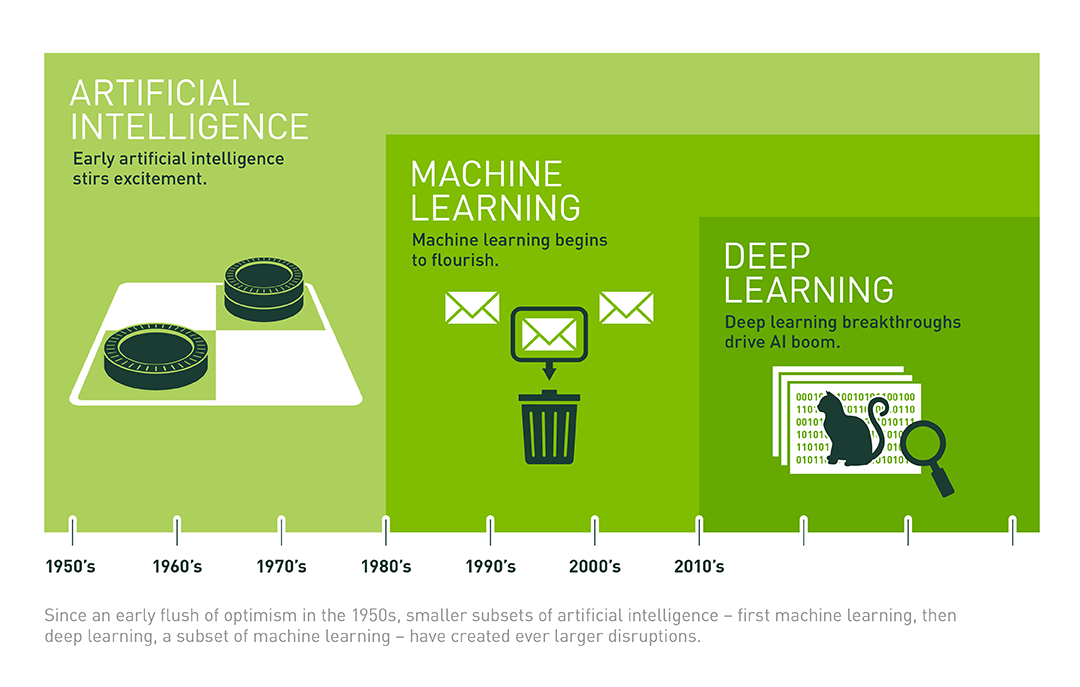
\includegraphics[width=\textwidth]{fig/L1/Deep_Learning_Icons_R5_PNG.png}
 \end{center}
 \rref[Source: NVidia]
 \end{frame}
 \begin{frame}{A (very) active field}
\begin{columns}
\column{.5\textwidth}
\begin{figure}
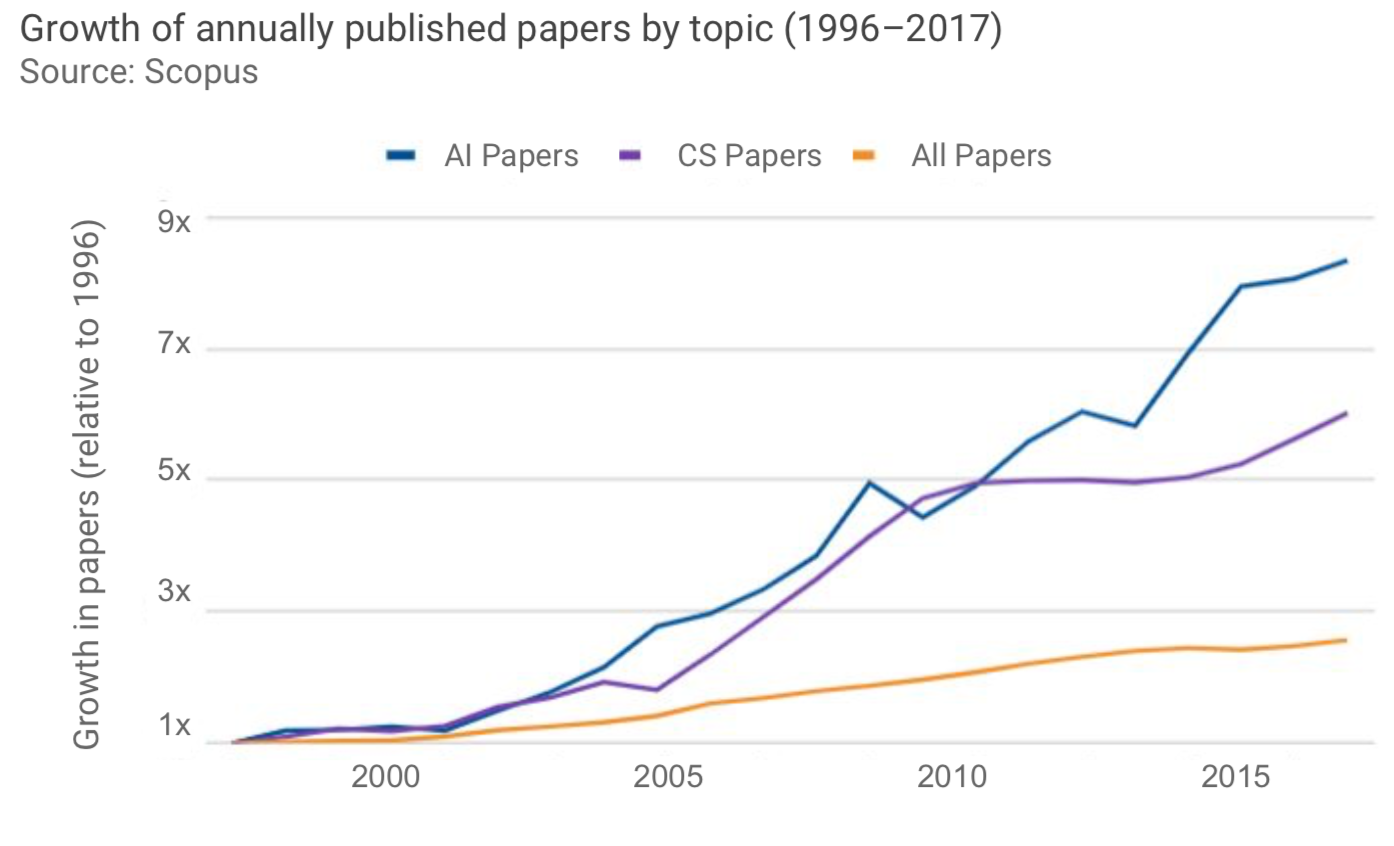
\includegraphics[width=\textwidth]{fig/L1/progress-papers.png}
\end{figure}
\column{.5\textwidth}

\begin{figure}
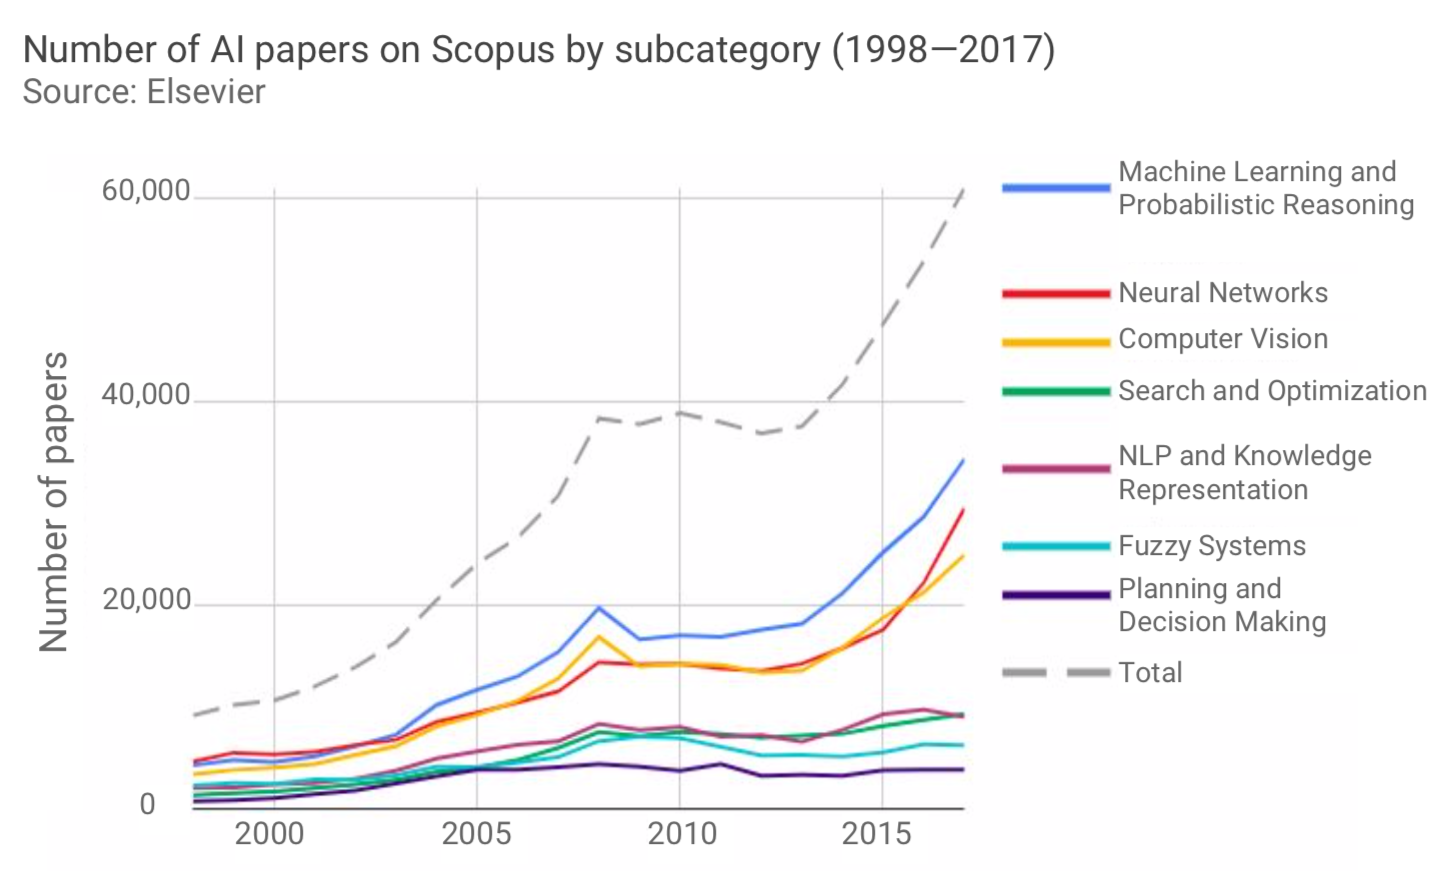
\includegraphics[width=\textwidth]{fig/L1/progress-ml.png}
\end{figure}
  \end{columns}
  \rref[Shoham et al., AI Index 2018 Annual Report]

\end{frame}



%%%%%%%%%%%%%%%%%%%%
\begin{frame}
\frametitle{Example 1: Computer Vision}
\begin{figure}
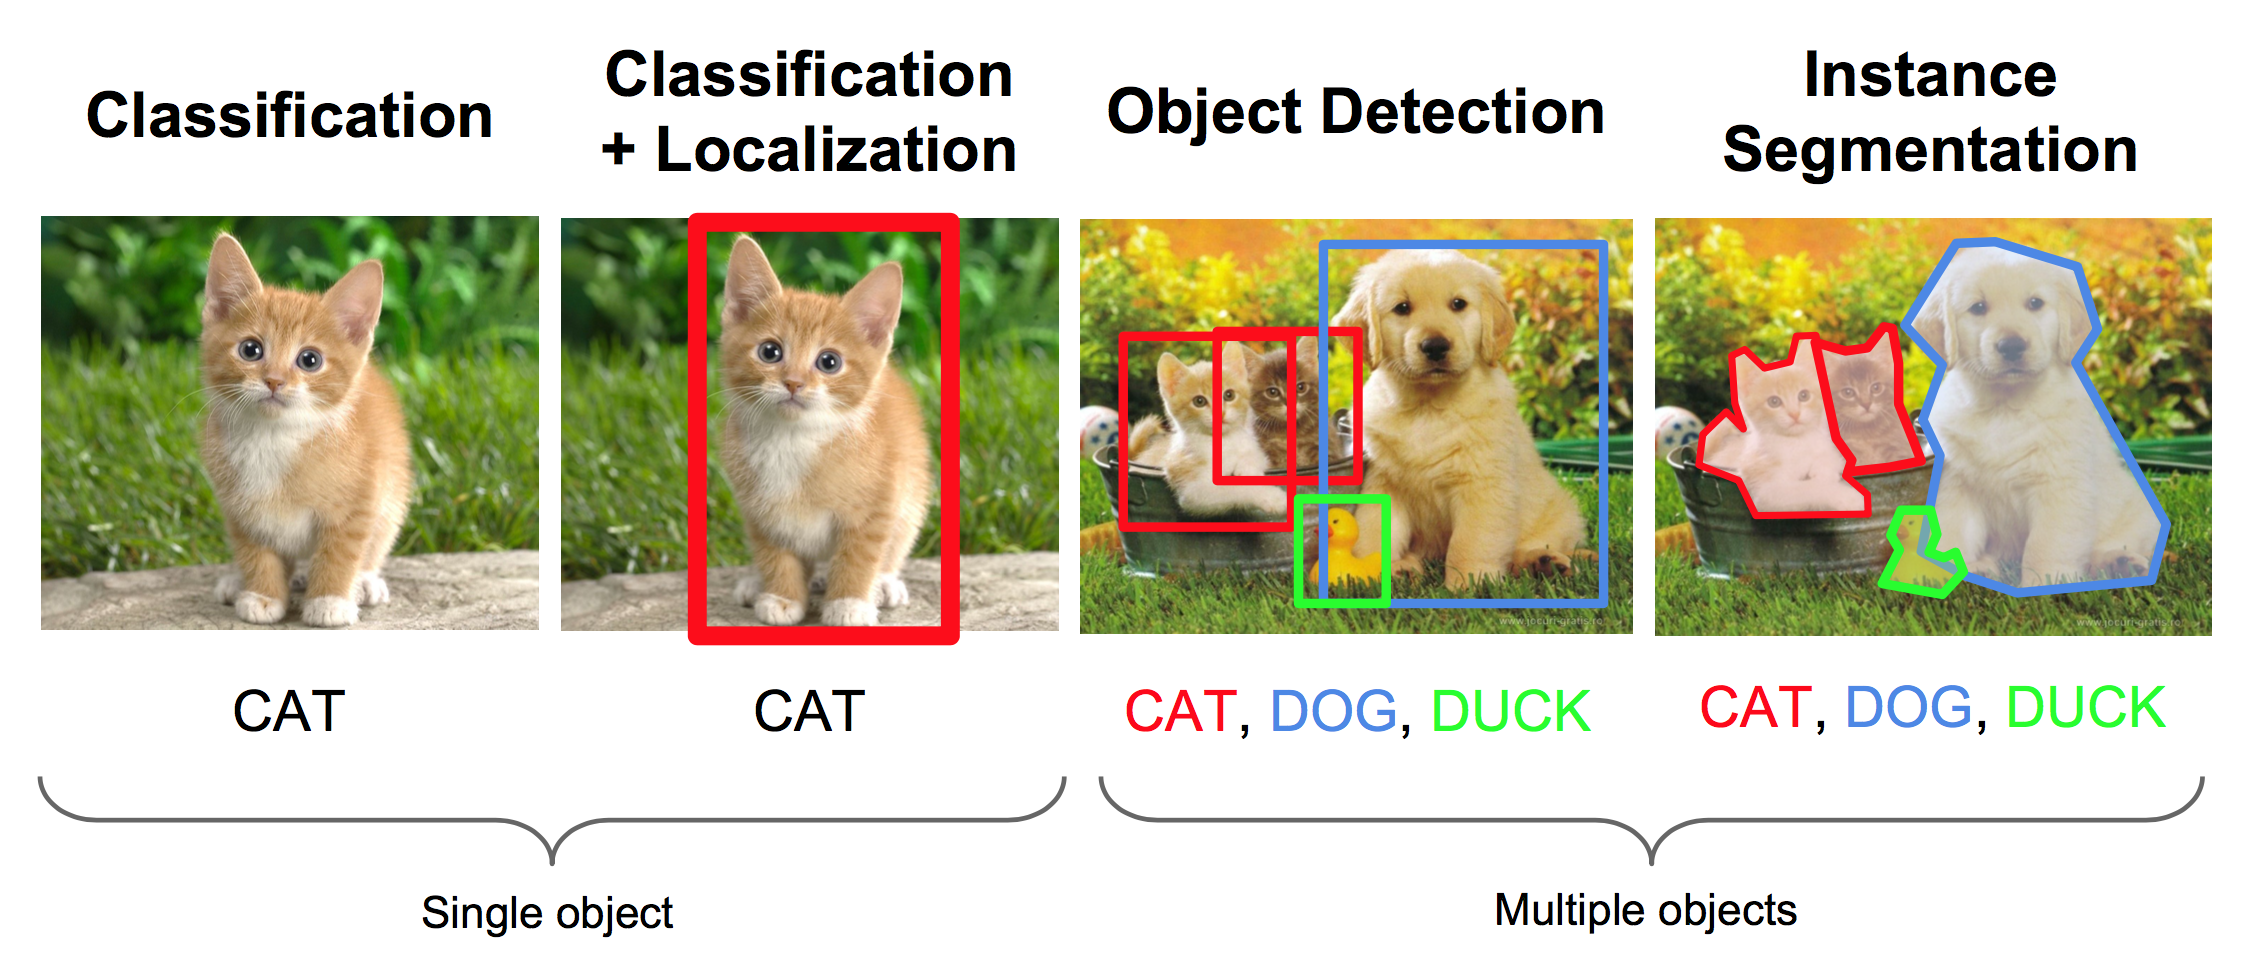
\includegraphics[width=\textwidth]{./fig/L1/compute-vision.png}
\end{figure}
\rref[Li, Karpathy and Johnson, 2016, Stanford CS231n course]

\end{frame}


%%%%%%%%%%%%%%%%%%%%
\begin{frame}
\frametitle{Example 1: Computer Vision}
\framesubtitle{Image Net Large Scale Recogonition Challenge (ILSVRC)}
\begin{figure}

\begin{tikzpicture} [scale=0.8, every node/.style={scale=0.6}]
  \begin{axis}[ 
    x tick label style={ 
      /pgf/number format/1000 sep=}, 
    ylabel=Classification error, 
    xtick={2010,2011,2012,2013,2014,2015,2016,2017},
    xticklabels={2010,2011,2012,2013,2014,2015,2016,hum.},
    enlargelimits=0.15, 
     bar width=7pt, 
    ybar,
   legend style={at={(0.5,-0.15)},
     anchor=north,legend columns=-1}, 
   x tick label style={font=\footnotesize,rotate=45, anchor=east},
   very axis plot/.append style={
      ybar,
      bar width=.2,
      bar shift=0pt,
      fill},
      nodes near coords,
   ] 
   \addplot[ybar,fill=blue!60, bar shift=0pt]
   coordinates {(2010,28) (2011,26)}; 
   \addplot[ybar,fill=red!60]
   coordinates {(2012,16) (2013,12) (2014,7) (2015,3.6) (2016,3)}; 
   \addplot[ybar,fill=green!60, bar shift=0pt] 
   coordinates 
   {(2017,5.1)};  
   \legend{traditional algo.,Deep Learning,Human}
 \end{axis} 
\end{tikzpicture}
\end{figure}
Deep learning architectures were based on Convolutional Neural Networks (CNN).
\end{frame}



%%%%%%%%%%%%%%%%%%%%
\begin{frame}
\frametitle{Example 2: Machine Translation}
Objective : translate a text from a language to another.
\begin{figure}

\includegraphics[width=.8\textwidth]{./fig/L1/google-trad.png}
\end{figure}
\begin{itemize}
\item {\bf Oct. 2013}: Pionneering scientic paper about neural networks in machine translation (Kalchbrenner, N., and Blunsom, P).
\item {\bf 2016}: Neural machine translation outperform tradiational approaches on public benchmarks
\item {\bf 2017}: Major systems (Google, Systran, WIPO, Microsoft) switch to
  neural machine translation  (using deep recurrent neural networks)
\end{itemize}
\end{frame}


%%%%%%%%%%%%%%%%%%%%
\begin{frame}
\frametitle{Example 3: Playing Games}
\begin{columns}
\column{.5\textwidth}
\begin{itemize}
\item {\bf 1997}: Deep Blue defeats Kasparov at Chess.
\item {\bf 2016}: AlphaGo's victory again Lee Sedol at Go.
\item {\bf 2017}: AphaGo Zero learns how to play Go only by playing against
  itself. It outperformed previous AlphaGo version (Reinforcement
  learning)
\item {\bf 2017}: DeepStack beats professional human poker players.
\end{itemize}
\column{.5\textwidth}
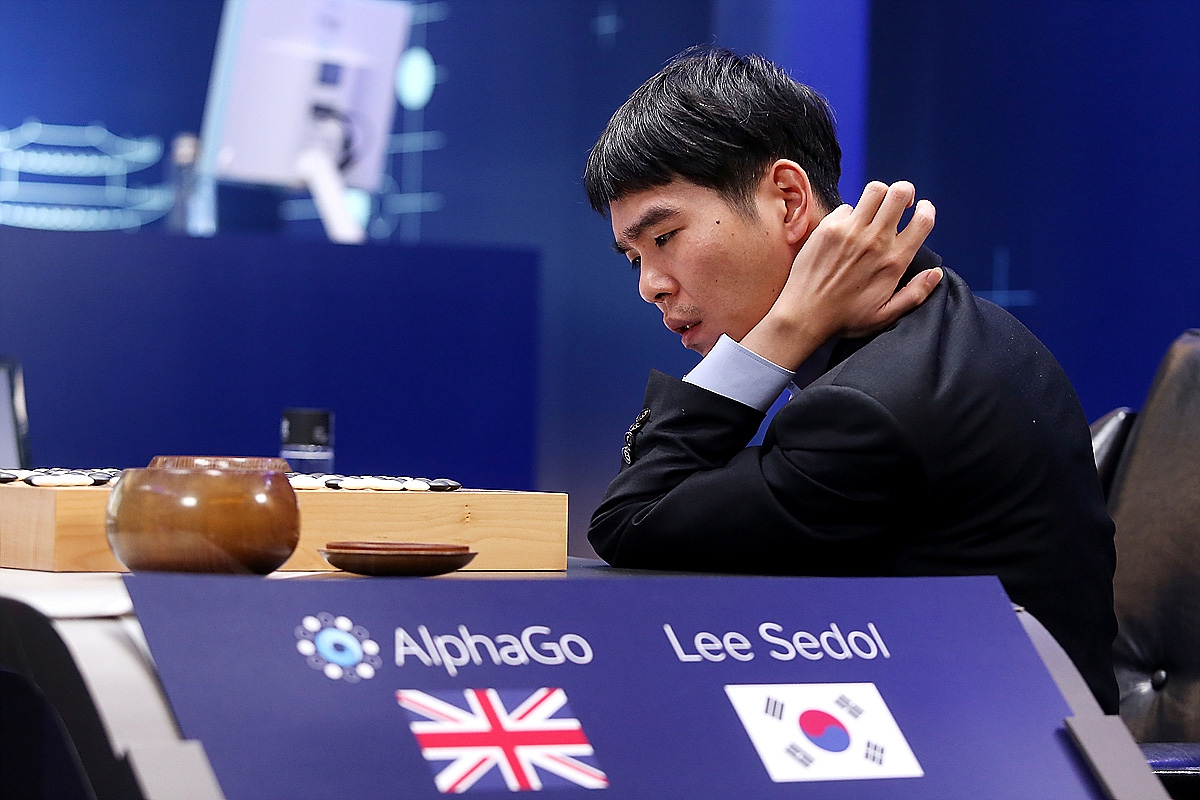
\includegraphics[width=\textwidth]{./fig/L1/alphago.jpg}
\end{columns}
\end{frame}

%%%%%%%%%%%%%%%%%%%%%
\begin{frame}{Predicting sport results?}
Rugby World Cup 2019
   \begin{figure}
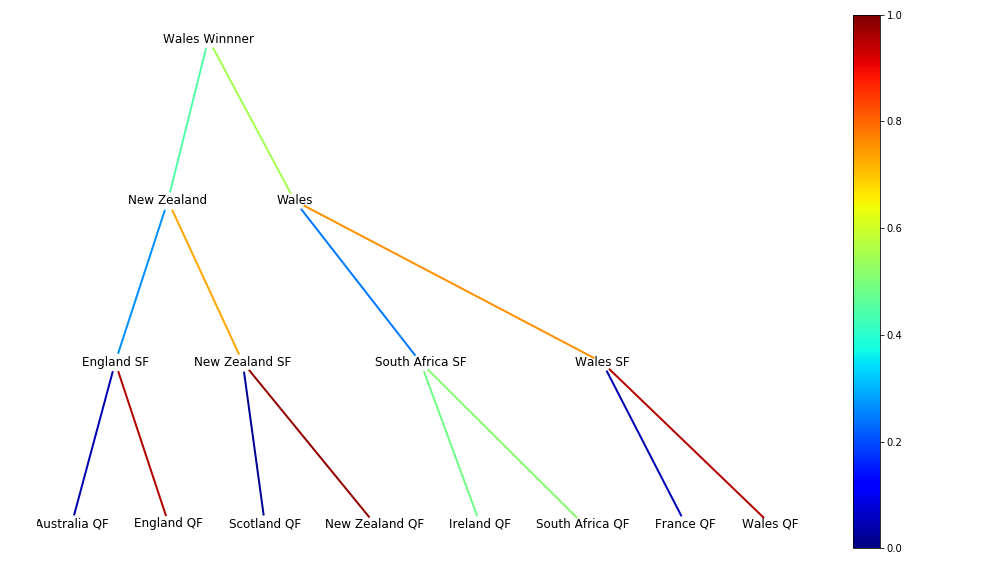
\includegraphics[width=.9\textwidth]{fig/L1/predicting-rugby.png} 
\end{figure}
Prediction based on XGBoost.
\begin{scriptsize}
   \url{https://towardsdatascience.com/predicting-the-winner-of-the-rugby-world-cup-2019-89a27d3f5b8e}
\end{scriptsize}

\end{frame}

\begin{frame}{AI Art?}
    \begin{figure}
        \centering
        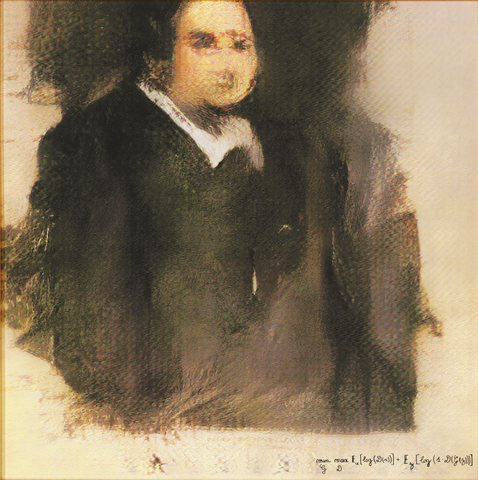
\includegraphics[width=0.5\textwidth]{fig/L3/478px-Edmond_de_Belamy.png}
        \caption*{\textit{Edmond de Bellamy} by Obvious(collective)}
    \end{figure}
    Generated using a Generative Adversarial Network.\\
    Selling prince (Oct. 2018): \$432,000
\end{frame}


%%%%%%%%%%%%%%%%%%%%%%%%
\begin{frame}[t]{Reasons for these recent achievements?}
    \begin{itemize}
        \item Increasing of the datasets in size and quality
        \only<1> {
        \begin{figure}
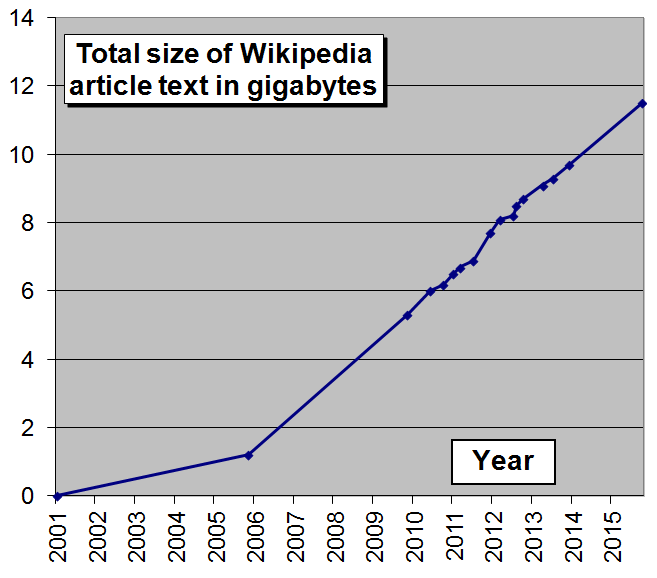
\includegraphics[width=.6\textwidth]{fig/L1/Wikipedia_article_size_in_gigabytes.png}
\end{figure}
\rref[source: Wikipedia]
}
        \item <2-> Progress in computing resources.
        \only<2> {
        \begin{figure}
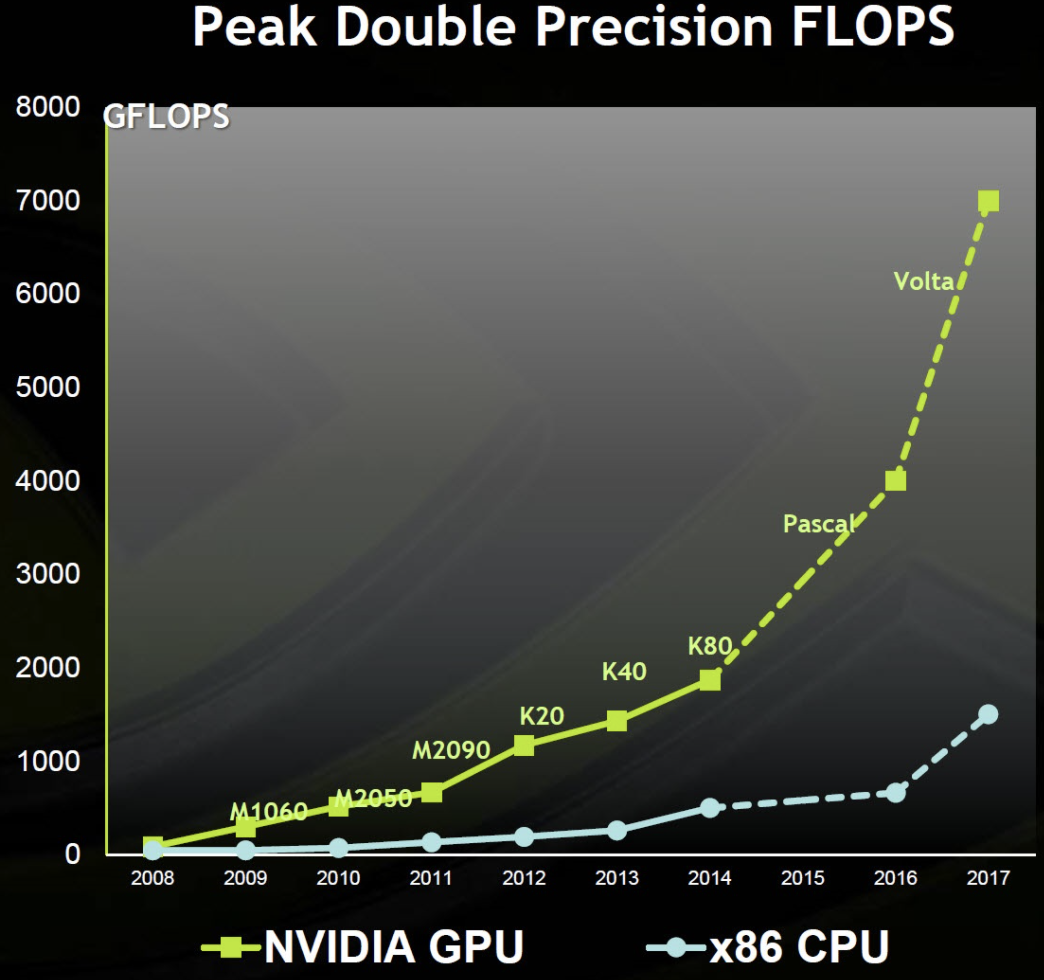
\includegraphics[width=.7\textwidth]{fig/L1/evolution-gpu.png}
\end{figure}
\rref[source: NVDIA]
}        
        
        \item <3-> Scientific research on new algorithms (e.g adapted to image processing)
                \only<3> {
        \begin{figure}
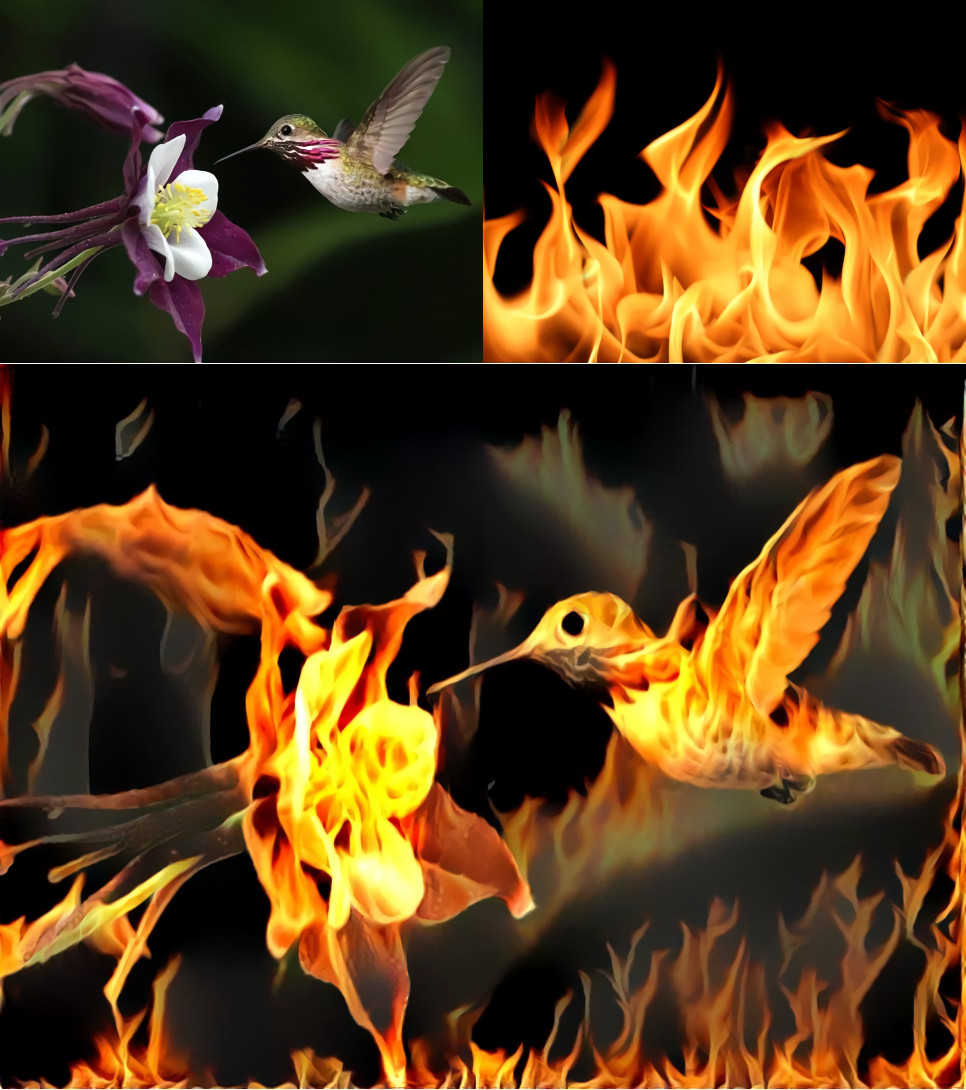
\includegraphics[width=.4\textwidth]{fig/L1/deep-art.jpg}
\end{figure}
\rref[source: Deep Dream Generator]

}        
    \end{itemize}

\end{frame}

\begin{frame}{Apply Machine-Learning to physical modelling?}
\alert{Why is it a good idea?}
    \begin{itemize}
        \item A increasing number of geophysical data (one spatial mission: 24 TB/day)
          \only<1> {
        \begin{figure}
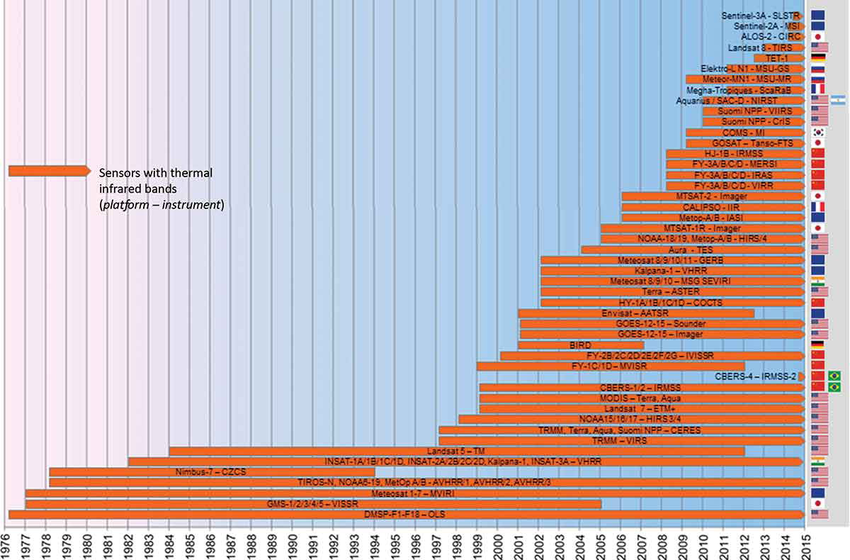
\includegraphics[width=.55\textwidth]{fig/L1/sat-sst.png}
\caption*{Satellites providing a semi-global daily coverage of surface temperature}
\end{figure}
\rref[source: Kuenzer et al. (2014)]
}
        \item <2->Data with highly significant spatial patterns
                  \only<2> {
        \begin{figure}
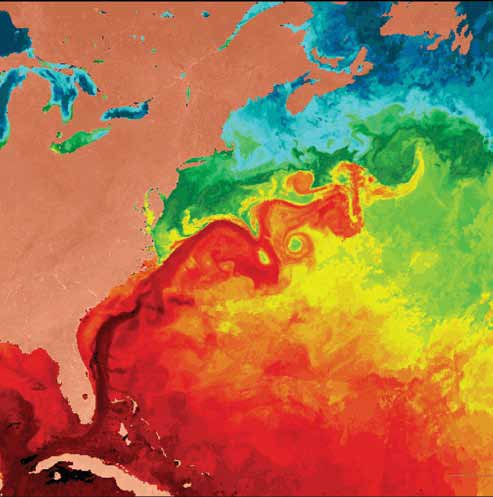
\includegraphics[width=.36\textwidth]{fig/L1/Satellite-image-of-sea-surface-temperature-showing-the-gulf-Stream-and-large-rings-and_W640.jpg}
\caption*{Sea Surface temperature of the gulf stream}
\end{figure}
\rref[source: Talley (2000)]
}
    \end{itemize}
\end{frame}

\begin{frame}{Why is physical modelling specific?}

\begin{columns}


\column{.5\textwidth}
\begin{figure}
    \caption*{NASDAQ Composite sock market index over the last 10 years}
    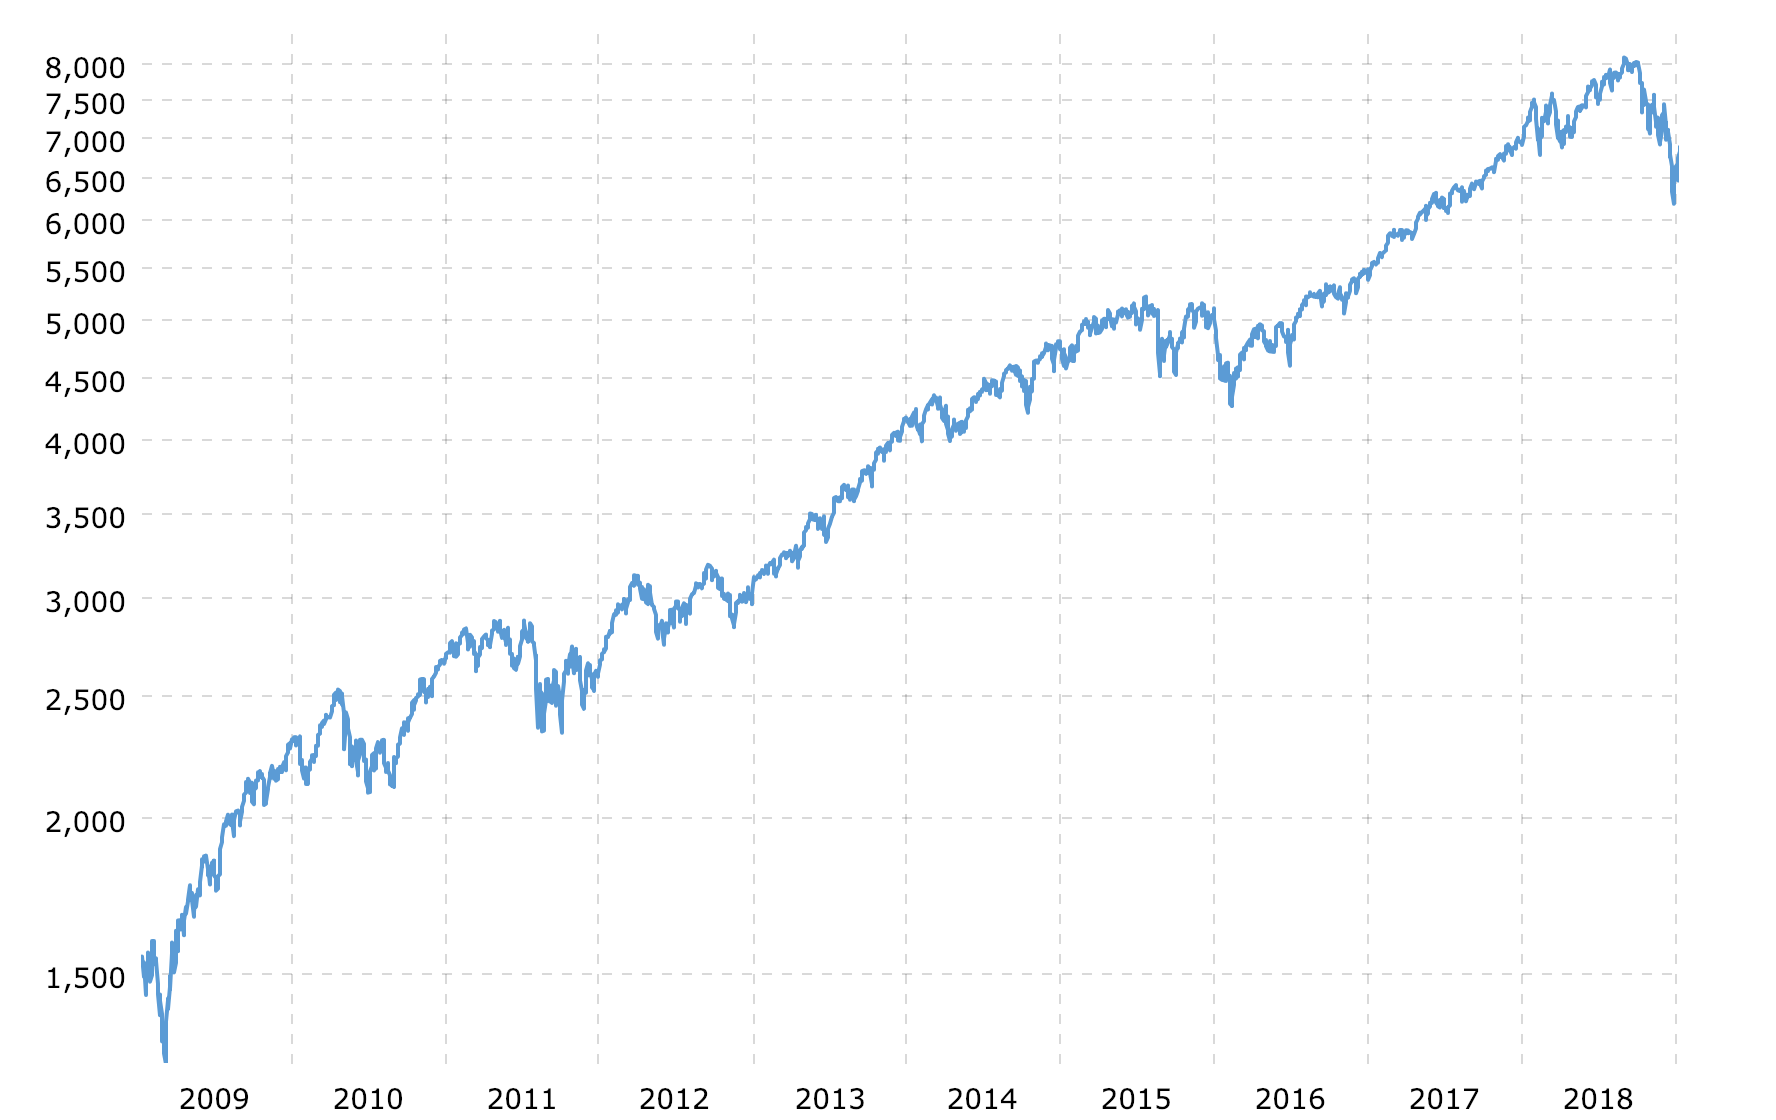
\includegraphics[width=\textwidth]{fig/L1/nasdaq-composite-index-10-year-daily-chart-2019-01-09-macrotrends.png}
\end{figure}
\visible<2->{\alert{Mostly unknown dynamical processes}}

\column{.5\textwidth}
\begin{figure}
    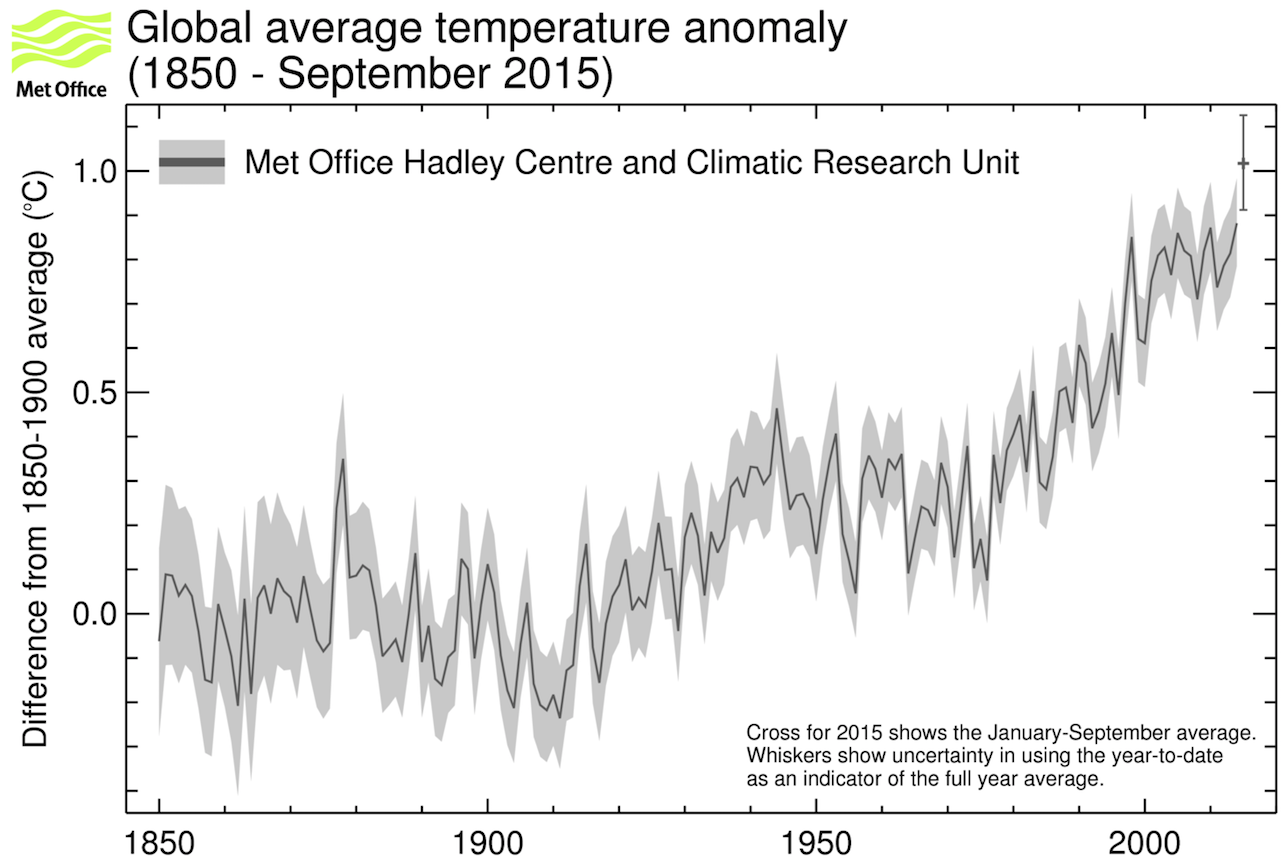
\includegraphics[width=\textwidth]{fig/L1/evolution-temperature.png}
\end{figure}
\visible<2->{\alert{Mostly known dynamical processes (based on physical principles)}}

\end{columns}
    
\end{frame}

\section{Generalities on Machine Learning}
%%%%%%%%%%%%%%%%%%%%%
\begin{frame}
\frametitle{What is this about ?}
\begin{alertblock}{Can we extract knowledge, make some predictions, determine a "model" using this large
amount of data ?}

\end{alertblock}
\pause
\begin{figure}
\begin{tikzpicture} [
	auto,
	node distance = 1cm]
	\node(H0) [anchor=east]{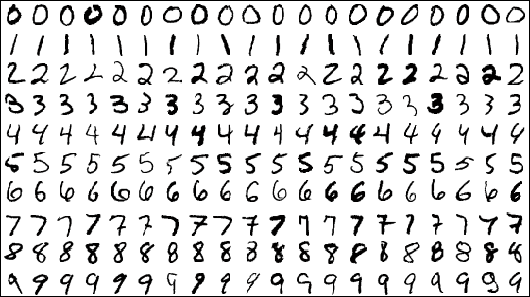
\includegraphics[width=0.4\textwidth]{./fig/L1/mnistExamples.png}};
	\node(H1) [right of =  H0, xshift = .4\textwidth]  
	{Digit \newline $\in \{0,\ldots,9\}$};
	\node(legend) [below of = H0,yshift=-4ex]{Base of images};
	\draw [very thick, ->] (H0)--(H1);
\end{tikzpicture}
\end{figure}
\pause
\begin{itemize}
\item From high dimensional data (thousands to millions dimensions) to reduced dimensional data (less than 100)
\item From disorganized data to comprehensive information
\item \alert{Can we teach a machine how to do that ?}
\end{itemize}

\end{frame}

%%%%%%%%%%%%%%%%%%%%%%%%%
\begin{frame}
\frametitle{Two classes of Machine Learning problems}
\begin{enumerate}
\item \alert{Regression}: Determination of a quantitative variable from a set of data
\begin{itemize}
\item The price of a building from various predictors (Surface, ...)
\item A physical value (Temperature, humidity, ...) in the future knowing the past
\item ...
\end{itemize}
\pause
\item \alert{Classification}: Determination of a class 
\begin{itemize}
\item A digit from a image
\item Identification of the content of an image
\item ...
\end{itemize}
\end{enumerate}
\end{frame}
%%%%%%%%%%%%%%%%%%%%%%%%%%%
\begin{frame}
\frametitle{Two types of objectives}

\begin{enumerate}[<+->]
\item \alert{Supervised learning}: we have a set of labeled data with examples of targets.
\item \alert{Unsupervised learning}: we only have unlabeled the data, we have no examples of
what we want to obtain. We want to extract a "useful" representation of these data, or
some coherent categories.
\begin{itemize}
\item Determine typical behaviors of clients in a supermarket knowing what the have bought.
\end{itemize}
\item \alert{Semi-Supervised Learning}: Only a few subset of the data are labeled
\item \alert{Reinforcement Learning}: We can initiate and observe the interaction of an agent with its environment. We want to optimize the behavior of the agent.
\begin{itemize}
\item Playing a chess game.
\end{itemize}
\end{enumerate}
\end{frame}

%%%%%%%%%%%%%%%%%%%%
\begin{frame}
\frametitle{Formally}
\begin{block}{A Machine}
\begin{equation*}
y = \mathcal{M}(x,\theta)
\end{equation*}
\begin{itemize}
\item $x$: input
\item $y$: output
\item $\mathcal{M}$: a model (named "machine")
\item $\theta$ : parameters of the model $\mathcal{M}$.
\end{itemize}
\end{block}
\alert{Machine learning} consists in optimizing $\theta$ using a set of data. 
This is the training process.
\end{frame}



%%%%%%%%%%%%%%%%%%%%
\begin{frame}
\frametitle{The Machine Learning recipe}
\begin{block}{A Machine}
\begin{equation*}
y = \mathcal{M}(x,\theta)
\end{equation*}
\end{block}
What are \alert{the ingredients}? 
\begin{columns}[t]

\column{.6\textwidth}

\begin{itemize}
    \item<2-> Some \alert{data}
    \begin{itemize}
        \item $x,y$ : supervised learning
        \item only $x$: unsupervised learning
        \item $x$ and some subset of $y$: semi-supervised learning
    \end{itemize}
    
    
    \item<3-> An \alert{objective}
        \begin{itemize}
\item $y$ is quantitative: regression
\item $y$ is a class: classification
    \end{itemize}
    \end{itemize}
    
\column{.6\textwidth}

\begin{itemize}
    \item<4-> A computational architecture (the \alert{machine})
        \begin{itemize}
        \item linear
        \item non-linear
        \item neural networks, random forest, ...
    \end{itemize}
    \item<5-> A \alert{learning} process
    \begin{itemize}
        \item Estimation of $\theta$
    \end{itemize}
\end{itemize}

\end{columns}

\end{frame}
%%%%%%%%%%%%%%%%%%
\begin{frame}{Multidimensional data}
Generally, we have multidimensional data $X$ and a one-dimensional target $y$.
\begin{figure}
\begin{tikzpicture}
\draw [fill=blue!20](0,0) rectangle (2,3);
\draw [fill=blue!20](2.5,0) rectangle (3.5,3);

\node [text centered] at (1,3.3) {features};
\node[text centered, rotate=90] at (-0.3,1.5) {samples};
\node [text centered] at (1,1.5) {\Large $X$};
\node [text centered] at (3,1.5) {\Large $y$};

  %\draw [fill=blue:20,black] (0.,0.) rectangle (1,2) ; 
\end{tikzpicture}
 \end{figure}
\end{frame}

%%%%%%%%%%%%%%%%%%%%
\begin{frame}{An illustration}
\begin{columns}
\column{.6\textwidth}
\begin{itemize}
    \item Some \alert{Data}
    \begin{figure}
    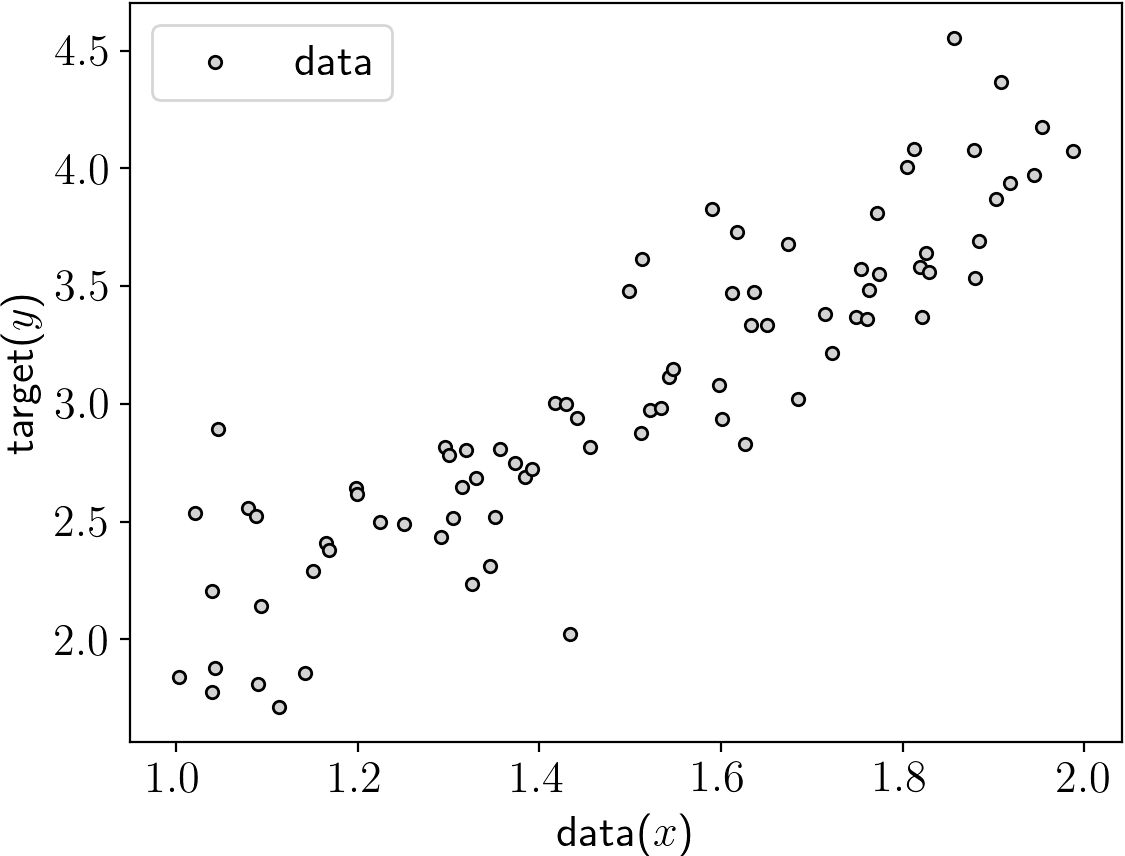
\includegraphics[width=.8\textwidth]{fig/L1/data-lin.png}
    \end{figure}

    \begin{itemize}
    \item $y$ is known: supervised learning
    \item $y$ is quantitative: regression
    \end{itemize}
\pause
\item An \alert{Objective}: Estimate $\hat{y}$ from $x$ by minimizing $(\hat{y}-{y})^2$ (Least-square objective)

\end{itemize}
\column{.5\textwidth}
\begin{itemize}
\pause
    \item A \alert{model}: $y = \theta_1 X + \theta_0$ (linear)
\pause
    \item A \alert{learning} process:
    $\mathbf{\theta}=(\mathbf{X}^T\mathbf{X})^{-1}\mathbf{X}^Ty$
\end{itemize}
\pause
\begin{block}{Result}
    \begin{figure}
    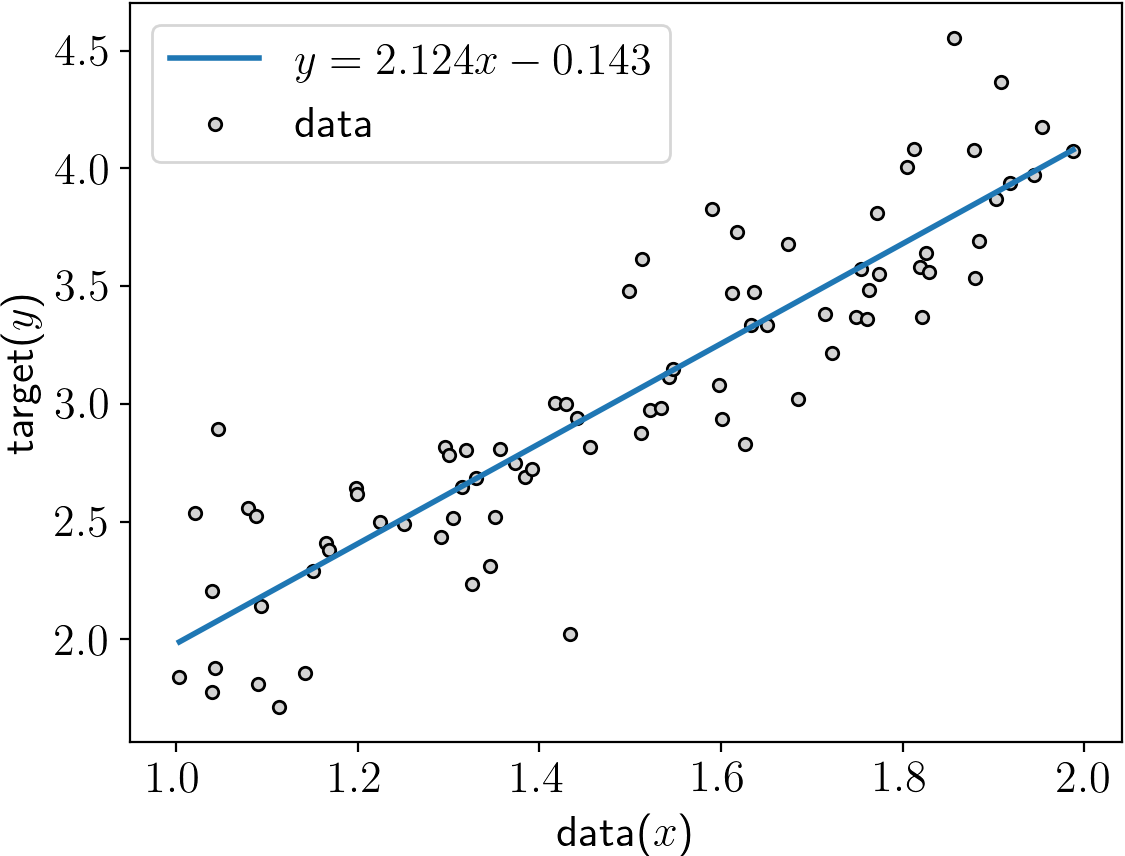
\includegraphics[width=.9\textwidth]{fig/L1/interp-lin.png}
    \end{figure}
\end{block}
\end{columns}
\end{frame}

%%%%%%%%%%%%%%%%%%%%
\section{Model selection/validation}

\begin{frame}{Choice of the model}
\begin{block}{Polynomial regression}
$y=\theta_0 + \theta_1 x + \theta_2 x^2 + \cdots + \theta_d x^d = \sum_{i=0}^d \theta_i X^i$
\end{block}
\begin{columns}
\column{.33\textwidth}
\pause
    \begin{figure}
    \caption*{degree = 1 (linear)}
    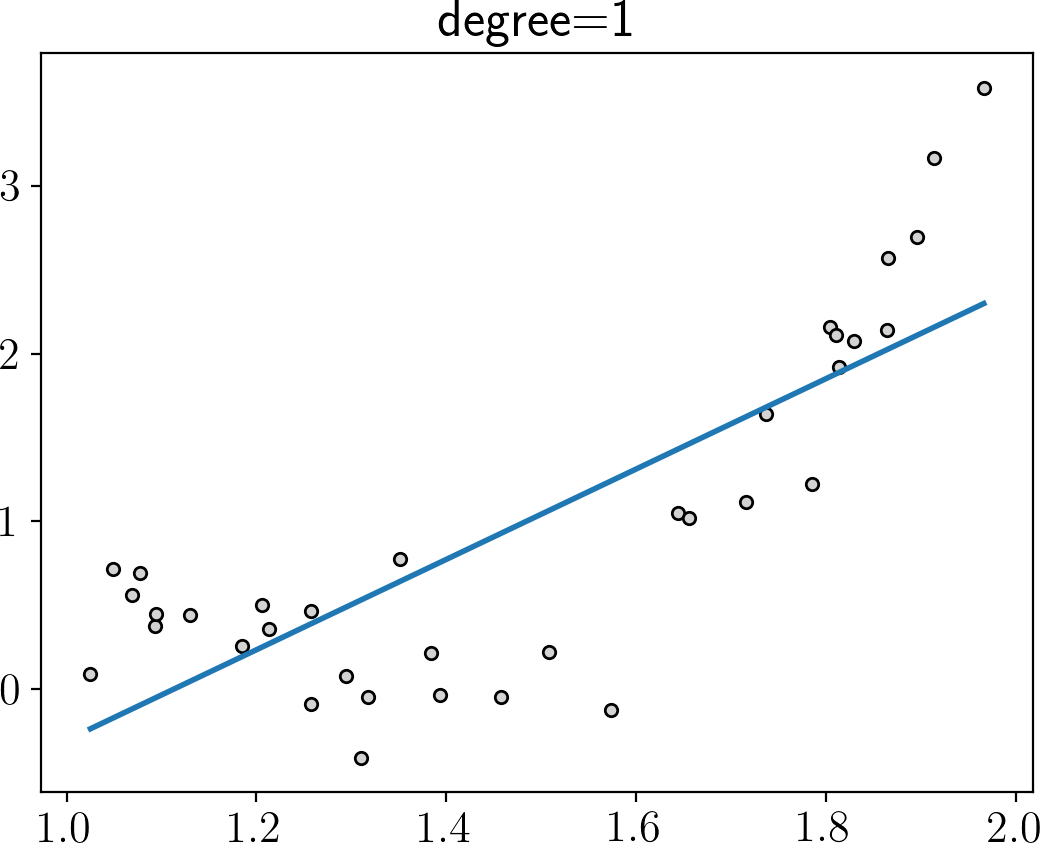
\includegraphics[width=\textwidth]{fig/L1/interp-pol-1.png}
    \end{figure}
\column{.33\textwidth}
\pause
    \begin{figure}
    \caption*{degree = 3 }
    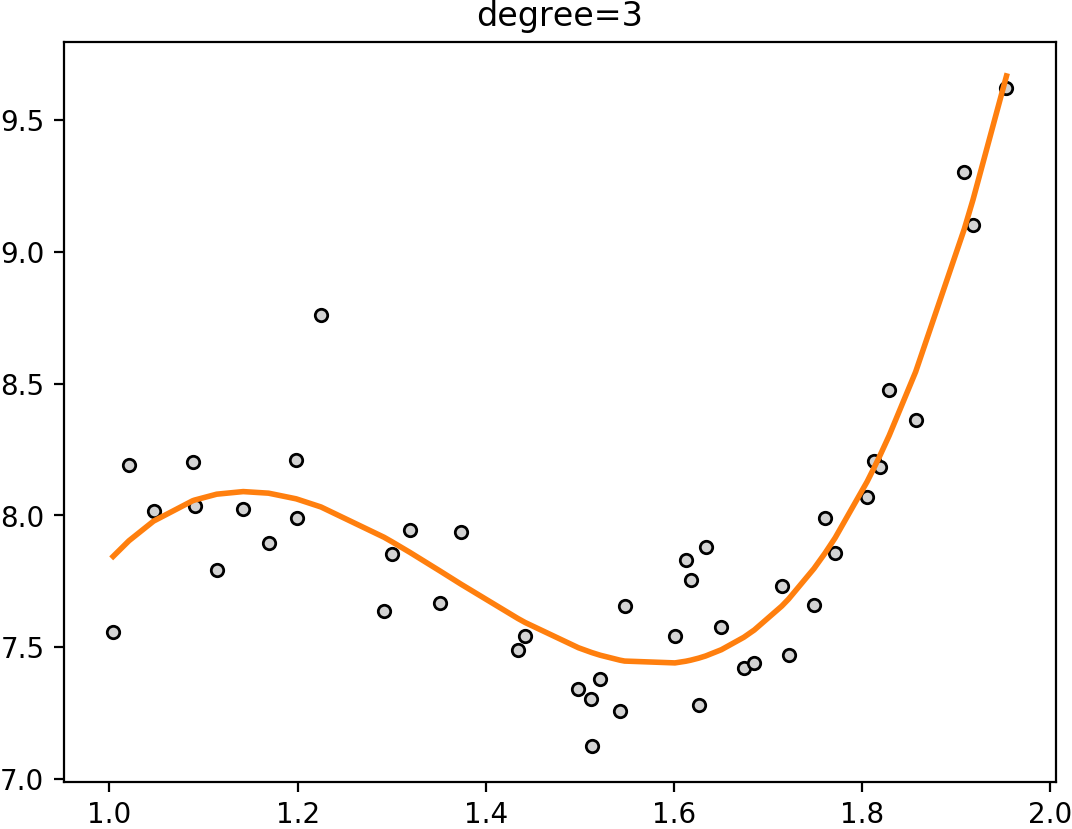
\includegraphics[width=\textwidth]{fig/L1/interp-pol-3.png}
    \end{figure}
\column{.33\textwidth}
\pause
    \begin{figure}
    \caption*{degree = 30 }
    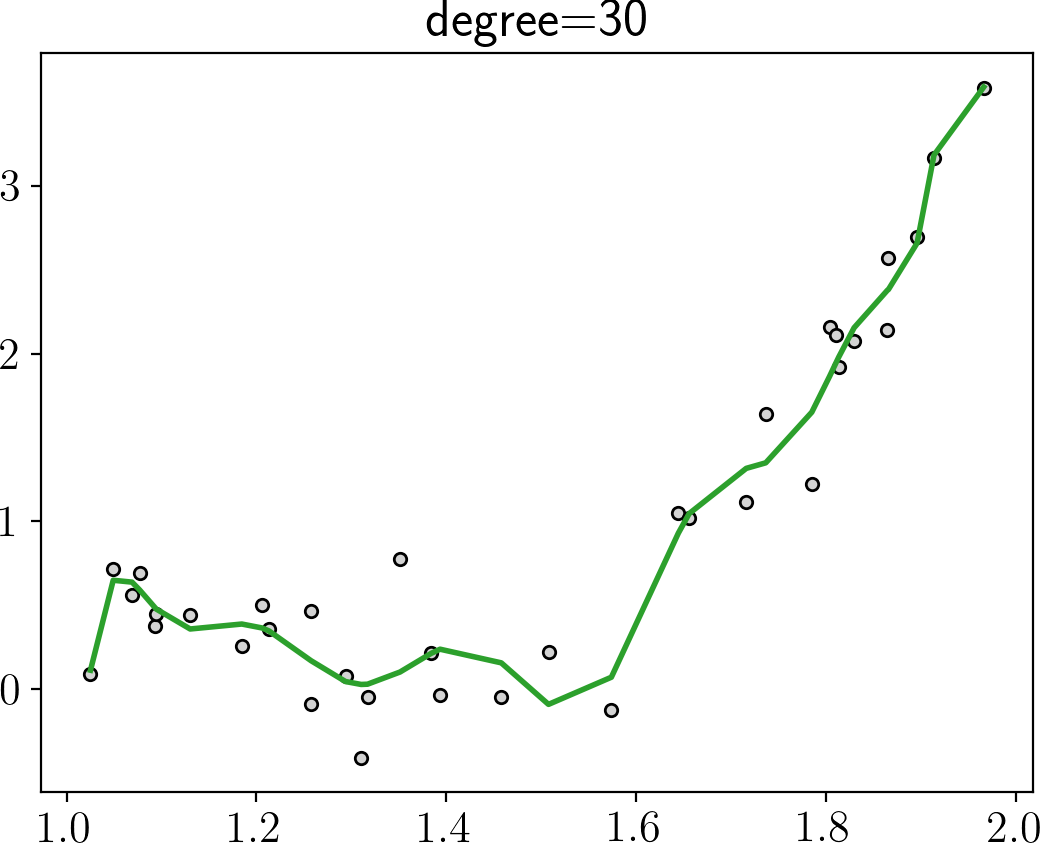
\includegraphics[width=\textwidth]{fig/L1/interp-pol-30.png}
    \end{figure}
 
\end{columns}
   
    \centering {
    \alert{What is the best model?}
    }
\end{frame}


%%%%%%%%%%%%%%%%%%%%
\begin{frame}{Train/Validation split}
\begin{block}{The idea}
Evaluate a score on a independent dataset
\end{block}
\pause
In our example we can randomly divide $(X,y)$ in two datasets:
\begin{itemize}
    \item The training dataset $X_{train},y_{train}$ used to fit the  model.
    \item The validation dataset $X_{val},y_{val}$ used to compute the score (e.g., correlation, mean-squared error)
\end{itemize}

    \begin{figure}
    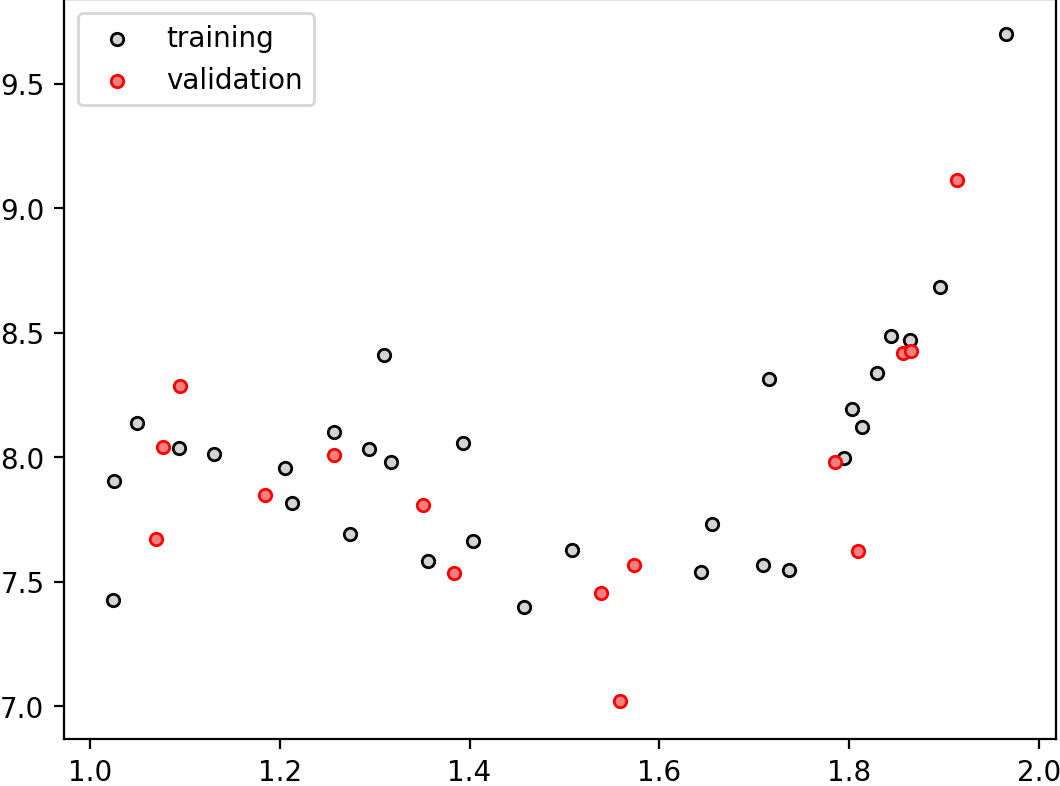
\includegraphics[width=.4\textwidth]{fig/L1/datasplit.png}
    \end{figure}

\end{frame}

%%%%%%%%%%%%%%%%%%%
\begin{frame}{Choice of the model}
\begin{columns}
\column{.5\textwidth}

    \begin{figure}
    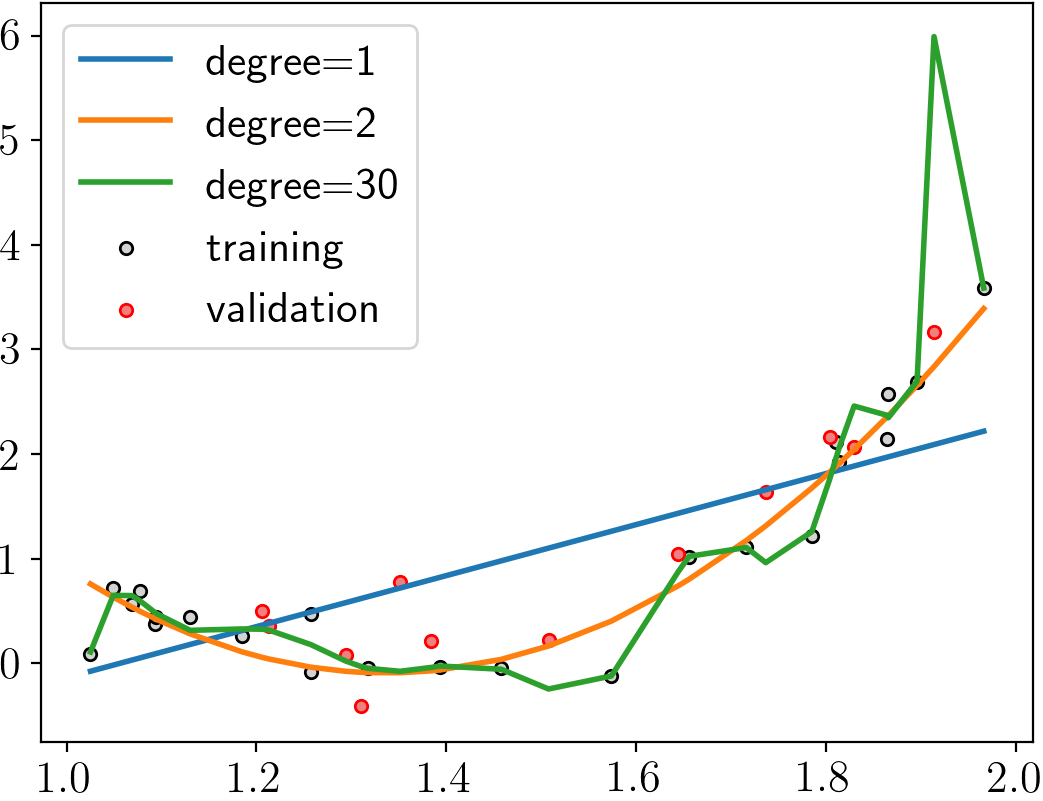
\includegraphics[width=\textwidth]{fig/L1/modelchoice.png}
    \end{figure}
\column{.5\textwidth}
Score: Mean Square Error (MSE)
\begin{table}
    \centering
    \begin{tabular}{c|c|c}
        Deg. & Train Score & Val. Score \\
        \hline
        1 & 0.17 & 0.23\\
        3 & 0.045 & 0.062\\
        30 & 0.035 & 0.27  \\
    \end{tabular}
    \end{table}
    %deg 1 ,score: val= 0.2283939842150192  , train= 0.167306864804612  , cv= 0.2768505679342689
%deg 3 ,score: val= 0.062492089527889656  , train= 0.04486320473714161  , cv= 0.05378120725339085
%deg 30 ,score: val= 0.27582336720042394  , train= 0.03473760406327127  , cv= 105306.65534552556
\end{columns}
\pause
   \begin{figure}
    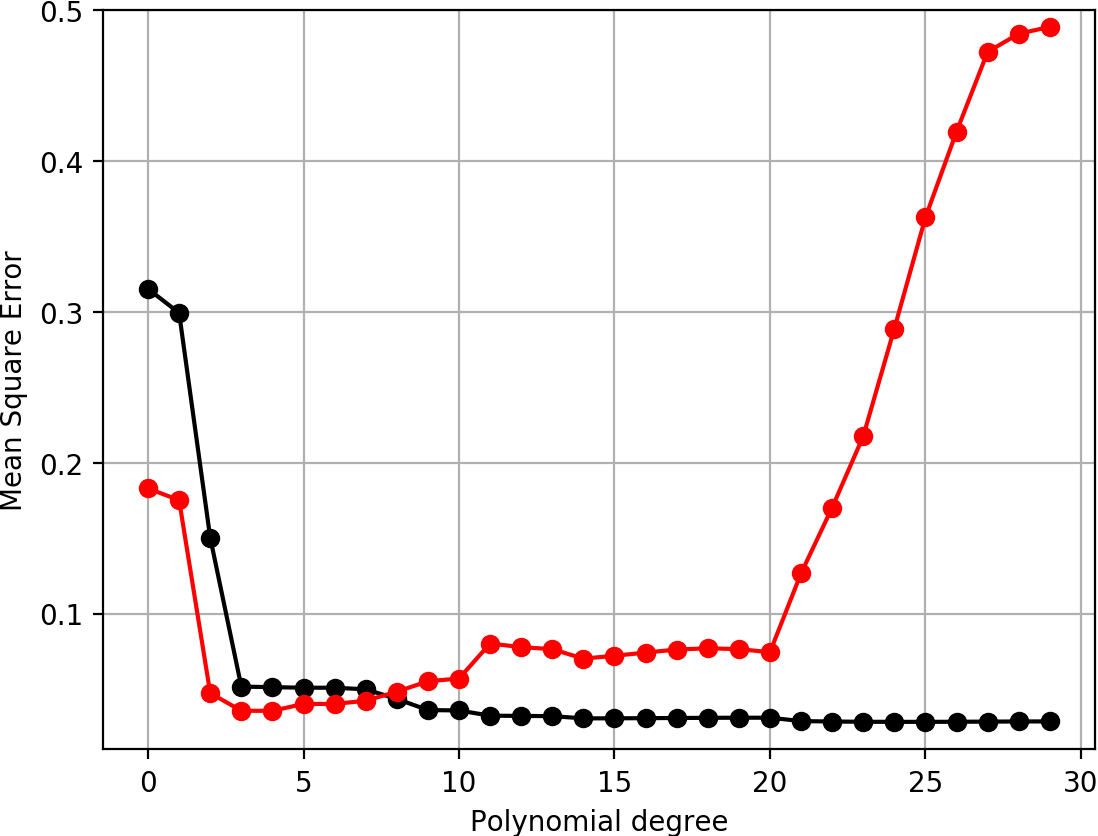
\includegraphics[width=.45\textwidth]{fig/L1/RMSE-deg-2scores.png}
    \end{figure}

\end{frame}

%%%%%%%%%%%%%%%%%%%%
\begin{frame}{Choice of the model}
\begin{block}{Polynomial regression}
$y=\theta_0 + \theta_1 x + \theta_2 x^2 + \cdots + \theta_d x^d = \sum_{i=0}^d \theta_i X^i$
\end{block}
\begin{columns}
\column{.33\textwidth}
    \begin{figure}
    \caption*{degree = 1 (linear)}
    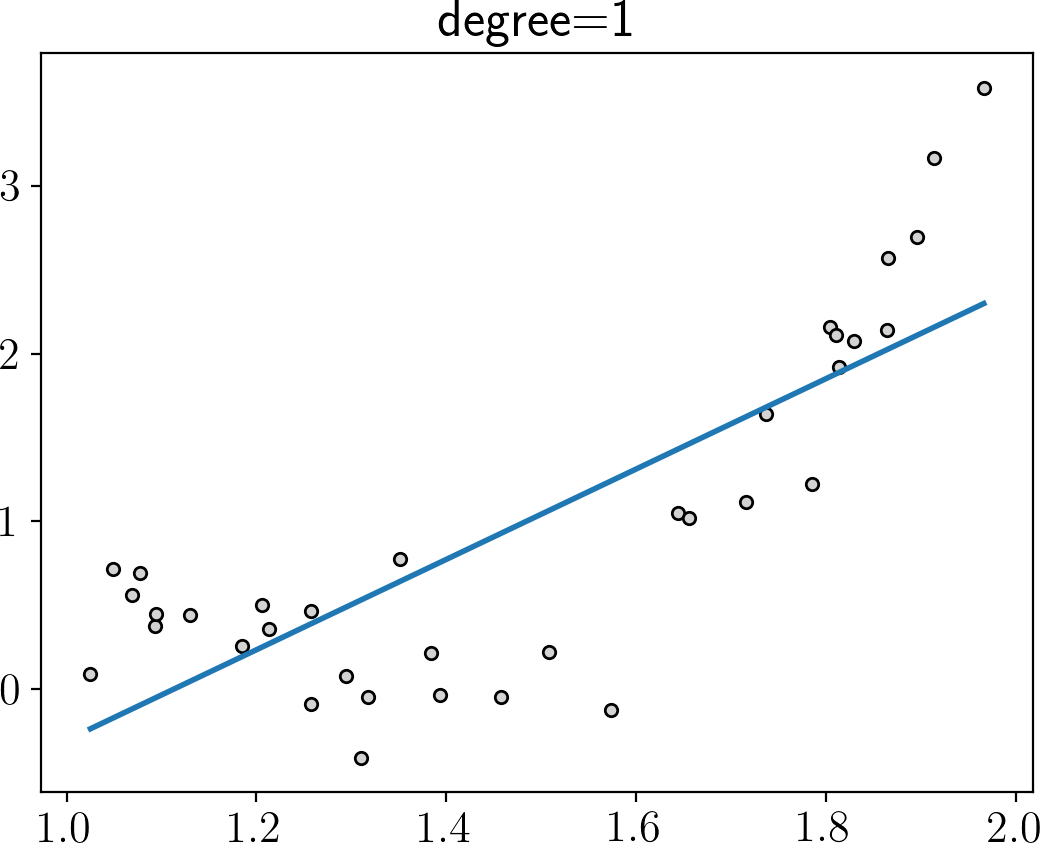
\includegraphics[width=\textwidth]{fig/L1/interp-pol-1.png}\\
        underfitting

    \end{figure}
\column{.33\textwidth}
    \begin{figure}
    \caption*{degree = 3 }
    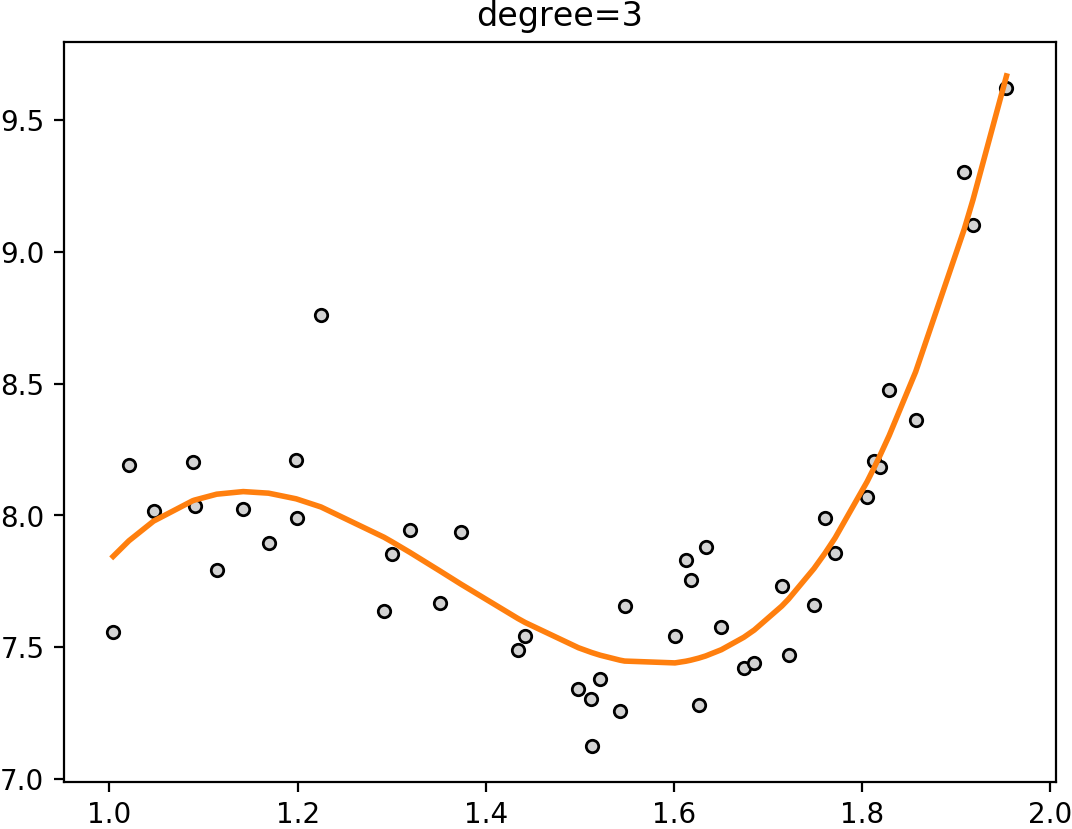
\includegraphics[width=\textwidth]{fig/L1/interp-pol-3.png}\\
        good fit

    \end{figure}
\column{.33\textwidth}
    \begin{figure}
    \caption*{degree = 30 }
    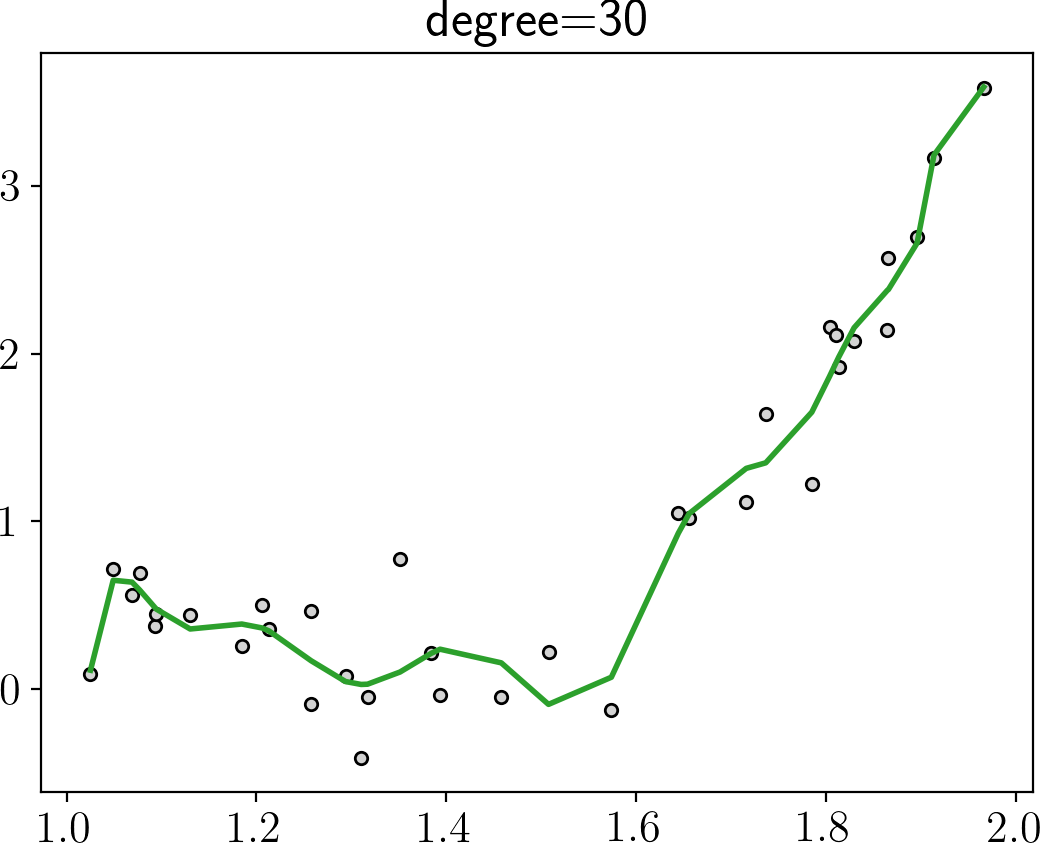
\includegraphics[width=\textwidth]{fig/L1/interp-pol-30.png}\\
        overfitting

    \end{figure}
 
\end{columns}

\end{frame}


%%%%%%%%%%%%%%%%%%%%
\begin{frame}{Train/Validation split}
     \begin{block}{Drawbacks}
\begin{itemize}
    \item drastically reduce the number of samples which can be used for learning the model
    \item Results  can depend on a particular random choice for the pair of (train, validation) sets.
\end{itemize}
\end{block}

\end{frame}
%%%%%%%%%%%%%%%%%%
\begin{frame}{More Robust: cross validation}
    \begin{block}{The idea}
    \begin{itemize}
\item Dividing the data in n folds, 
\item Learning n model (each time with a different training set),
\item Compute the mean score over n validation set.
\end{itemize}
\end{block}
   \begin{figure}
    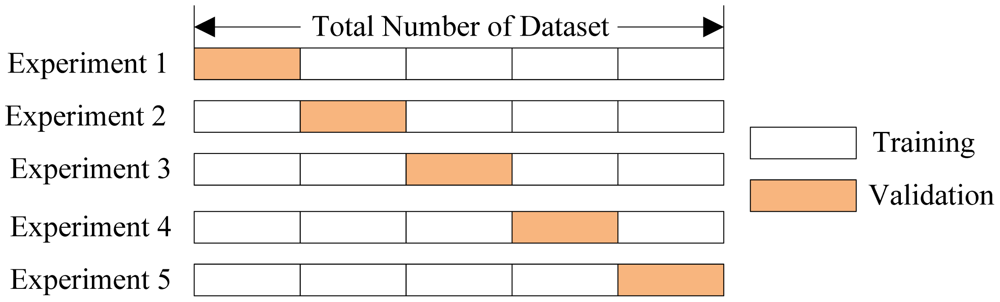
\includegraphics[width=\textwidth]{fig/L1/cv.png}
    \end{figure}

\end{frame}

%%%%%%%%%%%%%%%%%%%%
\begin{frame}{Cross-Validation}
\begin{columns}

\column{.3\textwidth}
\begin{table}
\footnotesize
    \centering
    \begin{tabular}{|c|c|}
    \hline
{\bf Fold} & {\bf MSE} \\
\hline
1 & 0.052 \\
2 & 0.043 \\
3 & 0.137 \\
4 & 0.025 \\
5 & 0.048 \\
6 & 0.144 \\
7 & 0.011 \\
8 & 0.025 \\
9 & 0.010 \\
10 & 0.028 \\
\hline
{\bf Mean} & {\bf 0.05} \\
        \hline


    \end{tabular}
    \end{table}
    
    \column{.7\textwidth}
   \begin{figure}
    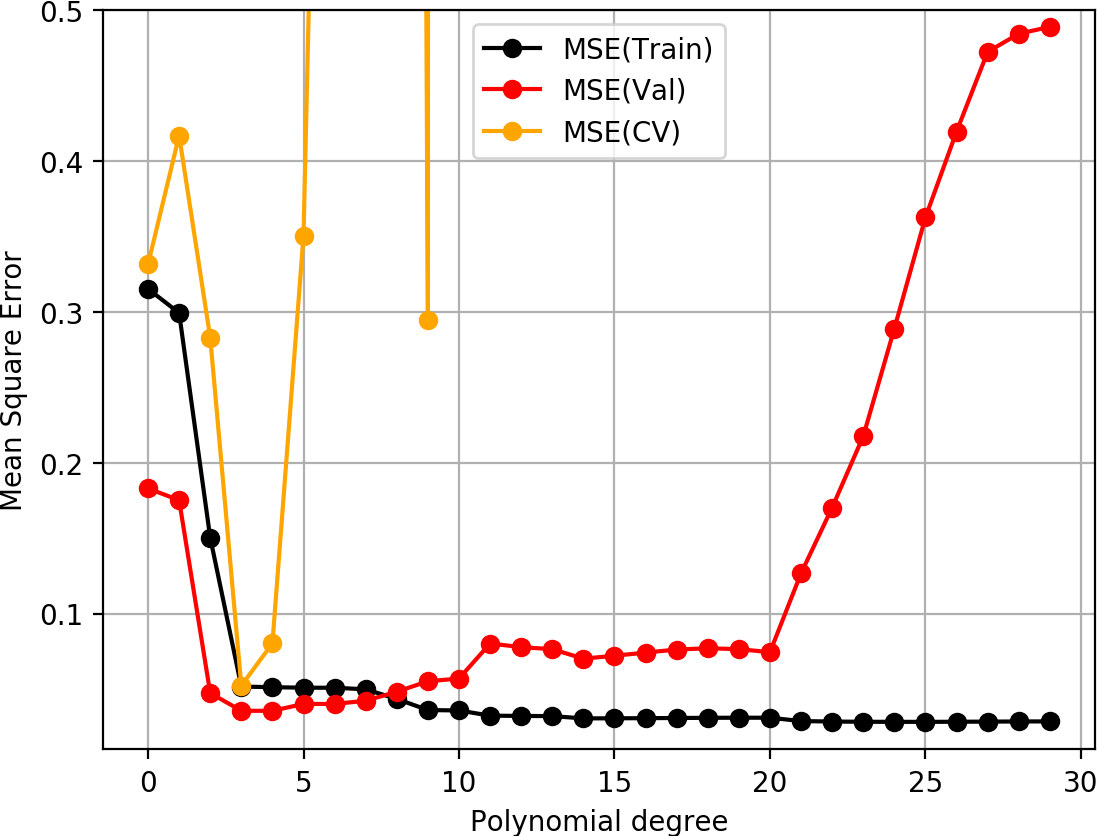
\includegraphics[width=\textwidth]{fig/L1/RMSE-deg-3scores.png}
    \end{figure}

\end{columns}

\end{frame}
%%%%%%%%%%%%%%%%
\begin{frame}{Wrapping up}
\begin{enumerate}[<+->]
    \item When applying machine learning techniques there are \alert{hyperparameters} to be determined (e.g., degree of the polynomial in polynomial regression).
    \item These \alert{hyperparameters}  can be determined by splitting the data into training/validation or by cross-validation.
    \item But then... the validation set was used to determine the best machine learning process
    \item To evaluate independanly the performance of our model, we should compute the score on a \alert{third independant dataset: The test dataset}.
    
\end{enumerate}
\pause
More on that in next lecture...

\end{frame}


%%%%%%%%%%%%%%%%
\begin{frame}{Data Leakage}

\begin{alertblock}{What is it?}
\alert{Data Leakage} is when information from outside the training dataset is used to create the model.
\end{alertblock}
\pause
Consequence: it can lead to overly optimistic models with no practical predictive skills.\\
\vspace{1em}
\pause
Example:
\begin{itemize}
    \item Using the future to make a forecast.
    \item Splitting between validation/training is not done properly
    \item Non-relevant features that can be related to the expected results (e.g. name/date of the files in a training dataset)
\end{itemize}
\end{frame}

%%%%%%%%%%%%%%%%%
\begin{frame}{Example of time series}
\begin{columns}

\column{.4\textwidth}
    \begin{figure}
    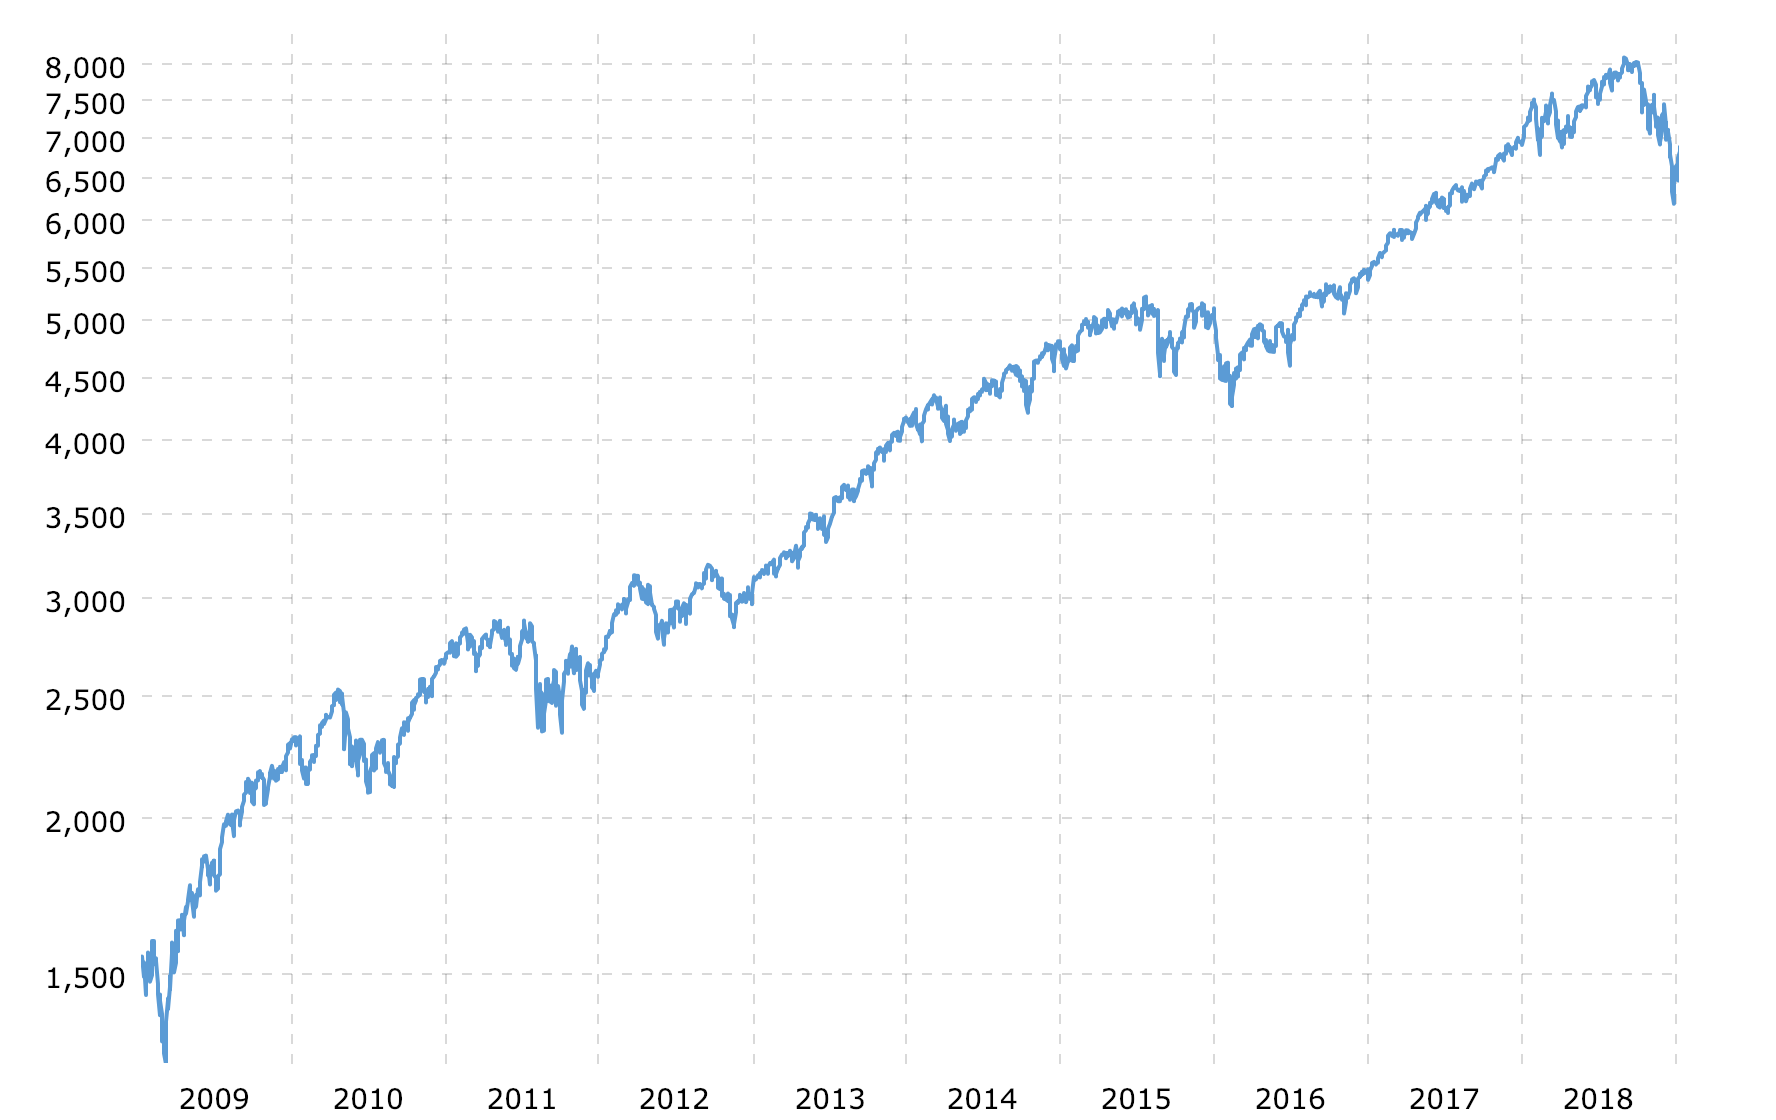
\includegraphics[width=\textwidth]{fig/L1/nasdaq-composite-index-10-year-daily-chart-2019-01-09-macrotrends.png}
    \end{figure}
\column{.6\textwidth}
\alert{Data:} $x_t$: NASDAQ index at the date $t$.\\
\alert{Objective:} predict $x_t$ given the index in the past ($x_0, \cdots , x_{t-1})$\\
\alert{A correct model:} $\hat{x}_t = \mathcal{M}(x_0, \cdots , x_{t-1},\theta)$\\
We can construct an incorrect model: $\hat{x}_t = \textcolor{red}{\mathcal{M^{\rm leak}}}(x_0, \cdots , x_{t-1},\textcolor{red}{x_t},\theta)$\\
$\textcolor{red}{\mathcal{M^{\rm leak}}}$ is perfect on the training set but is completely useless in practice.


\end{columns}

\end{frame}
%%%%%%%%%%%%%%%%%
\begin{frame}{More subtle example: contamination of the validation dataset}
\begin{columns}
\column{.6\textwidth}
\begin{center}
  \begin{tikzpicture}
    \node<1> (img1) {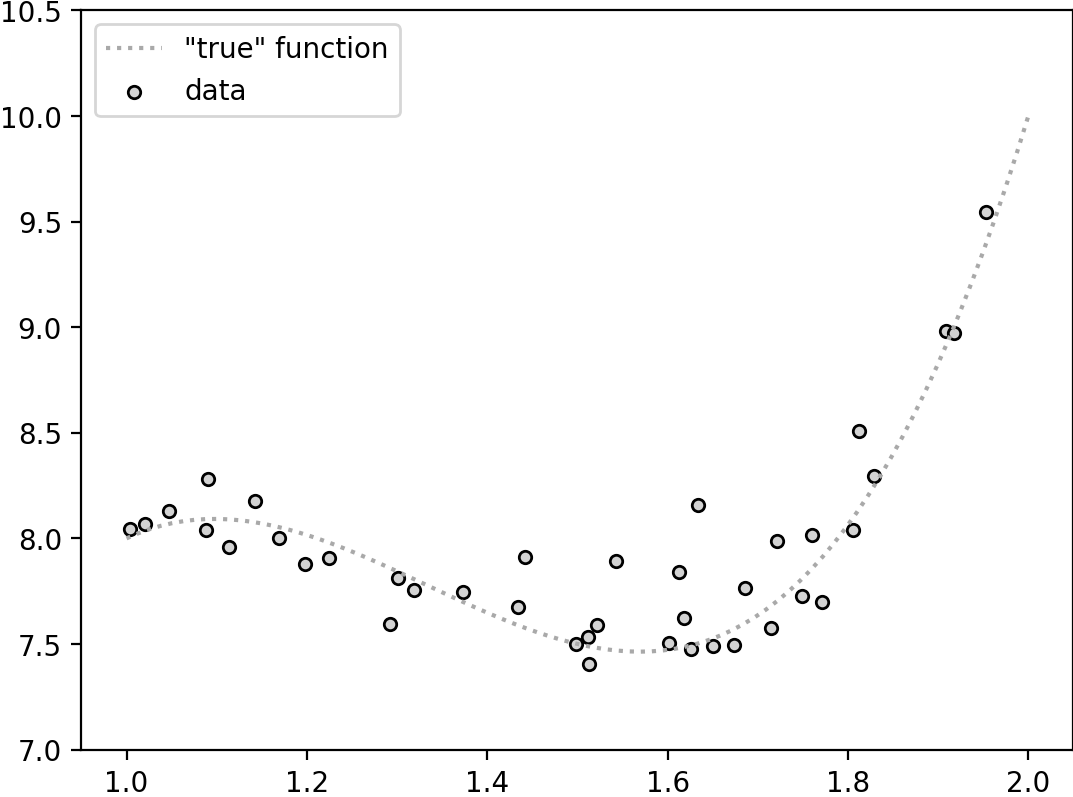
\includegraphics[width=\textwidth]{fig/L1/leakage-data.png}};
    \node<2-3> (img2) {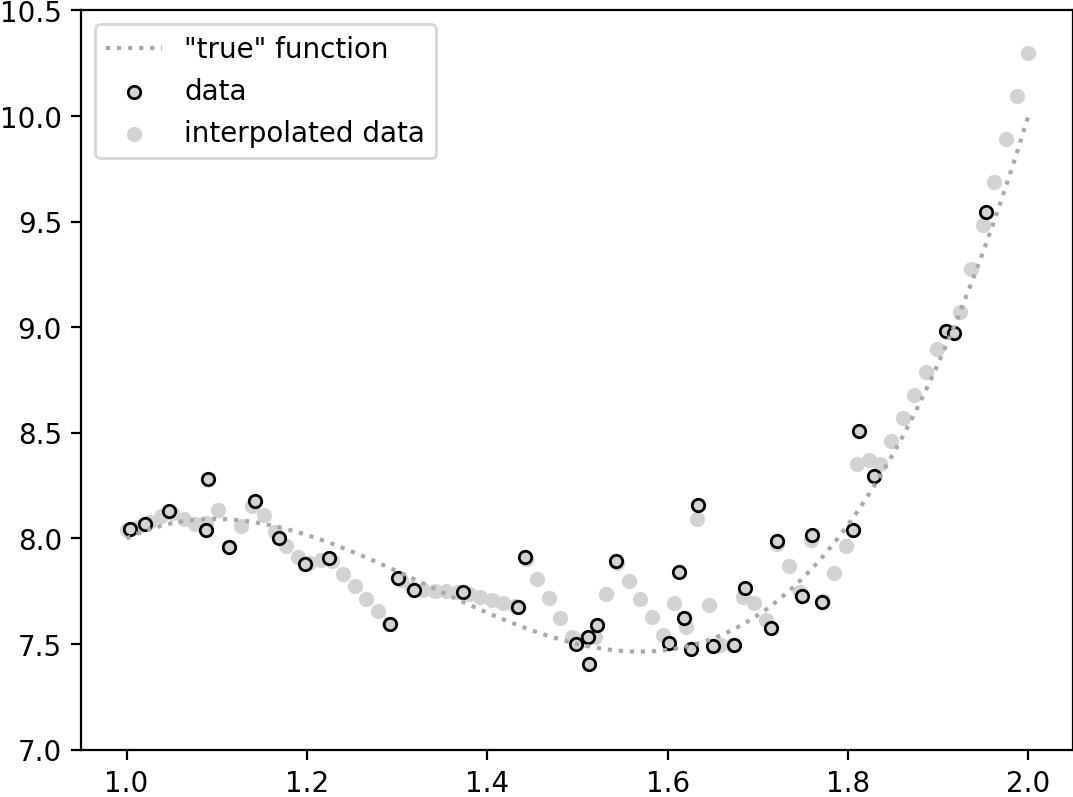
\includegraphics[width=\textwidth]{fig/L1/leakage-interp.png}};
    \node<4-> (img3) {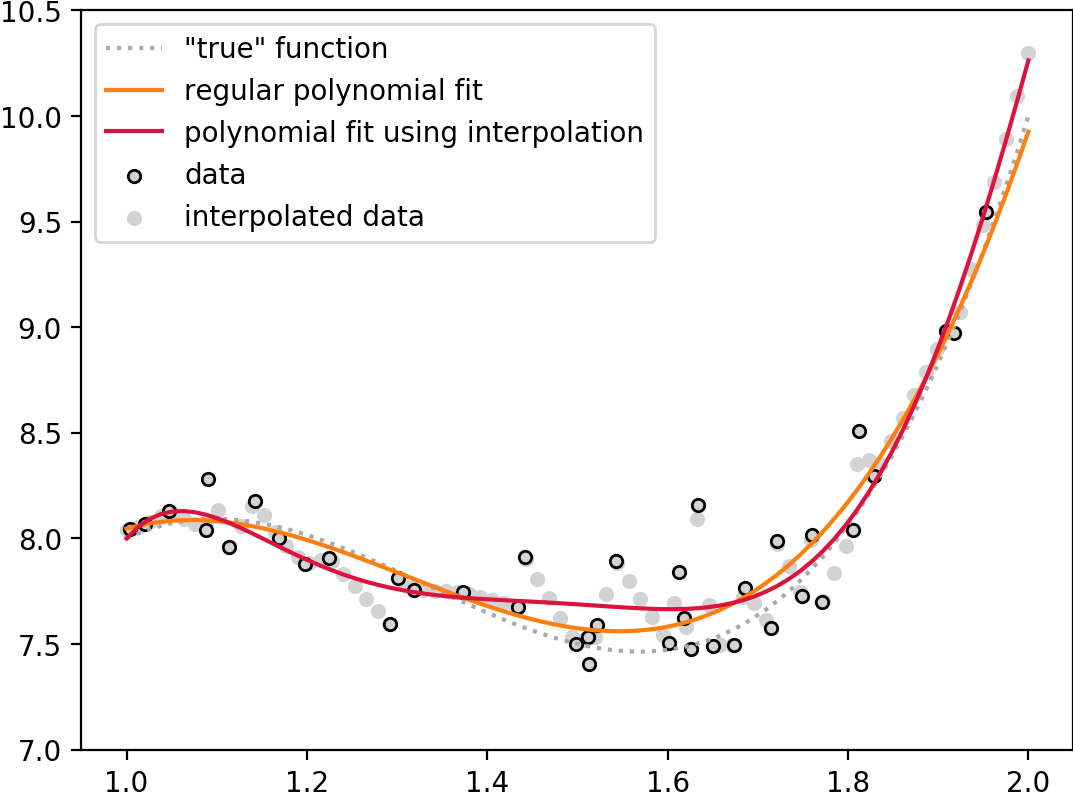
\includegraphics[width=\textwidth]{fig/L1/leakage-fit.png}};
  \end{tikzpicture}
\end{center}
\column{.4\textwidth}
\begin{figure}
    \centering
    \includegraphics<3->[width=\textwidth]{fig/L1/leakage-cv.png}

\end{figure}
\end{columns}

\begin{itemize}
    \item<1-> True polynom: $12x^3 - 48x^2 + 62x - 18$
    \item<5-> regular fit: $12x^3 - 49x^2 + 38x - 9$
    \item<5-> interpolated fit: $1143x^6 - 4803x^5 + 8242x^4 - 7446x^3 + 3736x^2 - 986x + 107 $
    
\end{itemize}
% raw:   array([-12.13896748,  49.07141924, -38.75248129,   9.86640163])
% interp: array([[-1143.54181925,  4803.98261307, -8242.31560901,  7446.33939621, -3735.92838024,   986.45002635,  -106.9868713 ]])

        
\end{frame}


%%%%%%%%%%%%%%%%%%
\begin{frame}{An example using scikit-learn}
    \begin{figure}
    \caption*{Boston House Prices}
    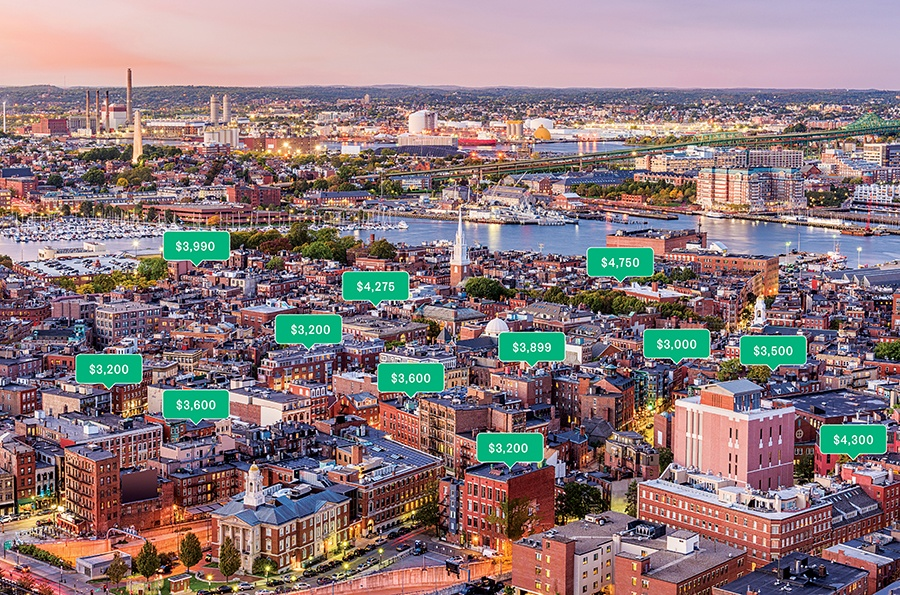
\includegraphics[width=.9\textwidth]{fig/L1/boston-rent.jpg}
    \end{figure}
\end{frame}

%%%%%%%%%%%%%%%%%%
\begin{frame}[fragile]{Questions addressed in this lecture}
    \begin{itemize}
        \item What are the more common area of application of machine learning? \cite[1]{Goodfellow-et-al-2016}
        \item What are the different class of ML problems? \cite[5.1]{VanderPlas-2016}
        \item What are the different types of learning (supervised, ...)?  \cite[5.1]{VanderPlas-2016}
        \item How to validate/select a model? \cite[5.3]{VanderPlas-2016}
        \item What is the cross-validation? \cite[5.3]{VanderPlas-2016}
        \item What is data leakage?
        {\footnotesize
        \href{https://machinelearningmastery.com/data-leakage-machine-learning/}{https://machinelearningmastery.com/data-leakage-machine-learning/}
        \href{https://www.kaggle.com/c/the-icml-2013-whale-challenge-right-whale-redux/discussion/4865\#25839}{https://www.kaggle.com/c/the-icml-2013-whale-challenge-right-whale-redux/discussion/4865\#25839}}
    \end{itemize}

\begin{footnotesize}
\begin{block}{Refs}
\cite[$n$]{VanderPlas-2016}: Jake VanderPlas, \textit{Python Data Science Handbook}, section $n$\\
\cite[$n$]{Goodfellow-et-al-2016}: Goodfellow etal., Deep Learning, chapter $n$
\end{block}
\end{footnotesize}
\end{frame}



%%%%%%%%%%%%%%%%%%%%%
%%%%%%%%%%%%%%%%%%%%%
%%%%%%%%%%%%%%%%%%%%%
%%%%%%%%%%%%%%%%%%%%%
%%%%%%%%%%%%%%%%%%%%%%%%%%%%%%%%%%%%%%%%%%
%%%%%%%%%%%%%%%%%%%%%
%%%%%%%%%%%%%%%%%%%%%%%%%%%%%%%%%%%%%%%%%%
\end{document}
%%%%%%%%%%%%%%%%%%%%%%%%%%%%%%%%%%%%%%%%%%




\begin{frame}
\frametitle{Example of a non-linear relationship}
\begin{figure}
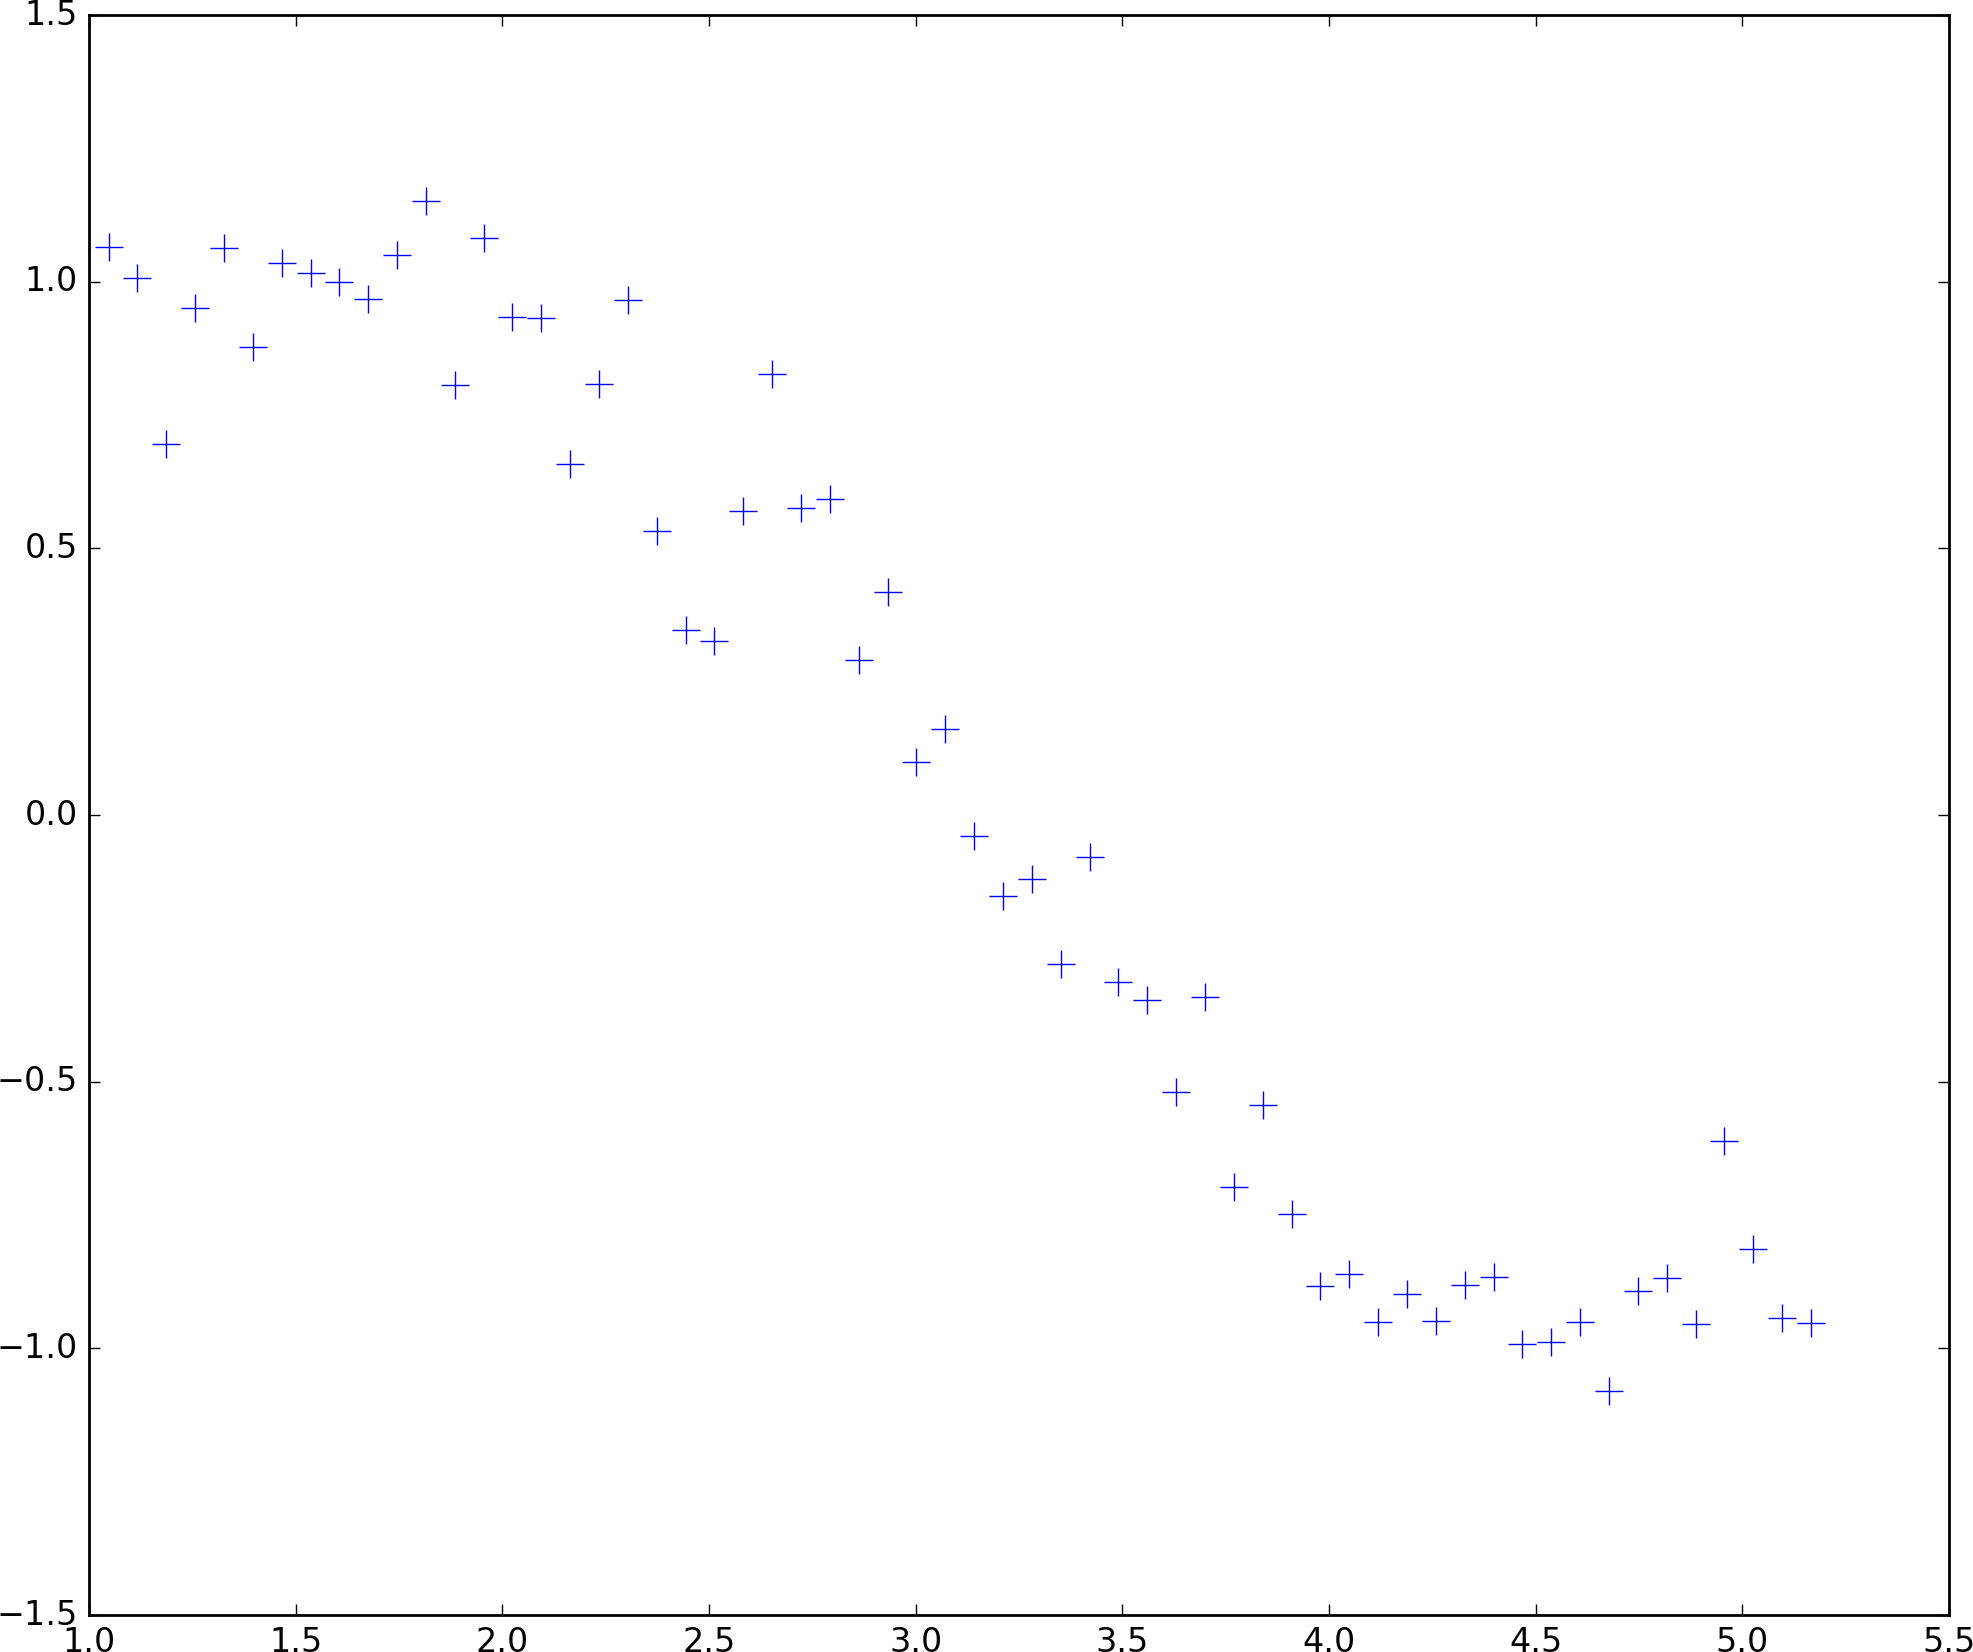
\includegraphics[height=0.55\textheight]{./fig/L1/scatter.png}
\end{figure}
\begin{block}{An idea}
We could take an polynomial hypothesis model:
$$
h_{\bm{\theta}}(x) = \theta_0 x^0 + \theta_1 x^1 + \ldots + \theta_p x^p
$$
\end{block}
\end{frame}
%%%%%%%%%%%%%%%%%%%%%
\begin{frame}
\frametitle{Example}
$\{(x_1,y_1),\ldots,(x_n,y_n)\}$ is the learning dataset.

For a given polynom degree $p$, parameters $\bm{\theta}$ are determined minimizing the 
least-mean square cost function:
$$
J(\bm{\theta}) = \frac{1}{n} \sum (y_i - h_{\bm{\theta}}(x_i))^2
$$
with $h_{\bm{\theta}}(x) = \theta_0 x^0 + \theta_1 x^1 + \ldots + \theta_p x^p$
\begin{itemize}[<+->]
\item It can be determined using a gradient descent method
\item If the degree of the polynom $p=1$, it is a simple linear regression
\end{itemize}
\end{frame}
%%%%%%%%%%%%%%%%%%%%%
\begin{frame}
\frametitle{A first result}
\vspace{-2em}
\begin{columns}[t]
\column{.5\textwidth}
\begin{figure}
$p=1$ (linear regression)\\
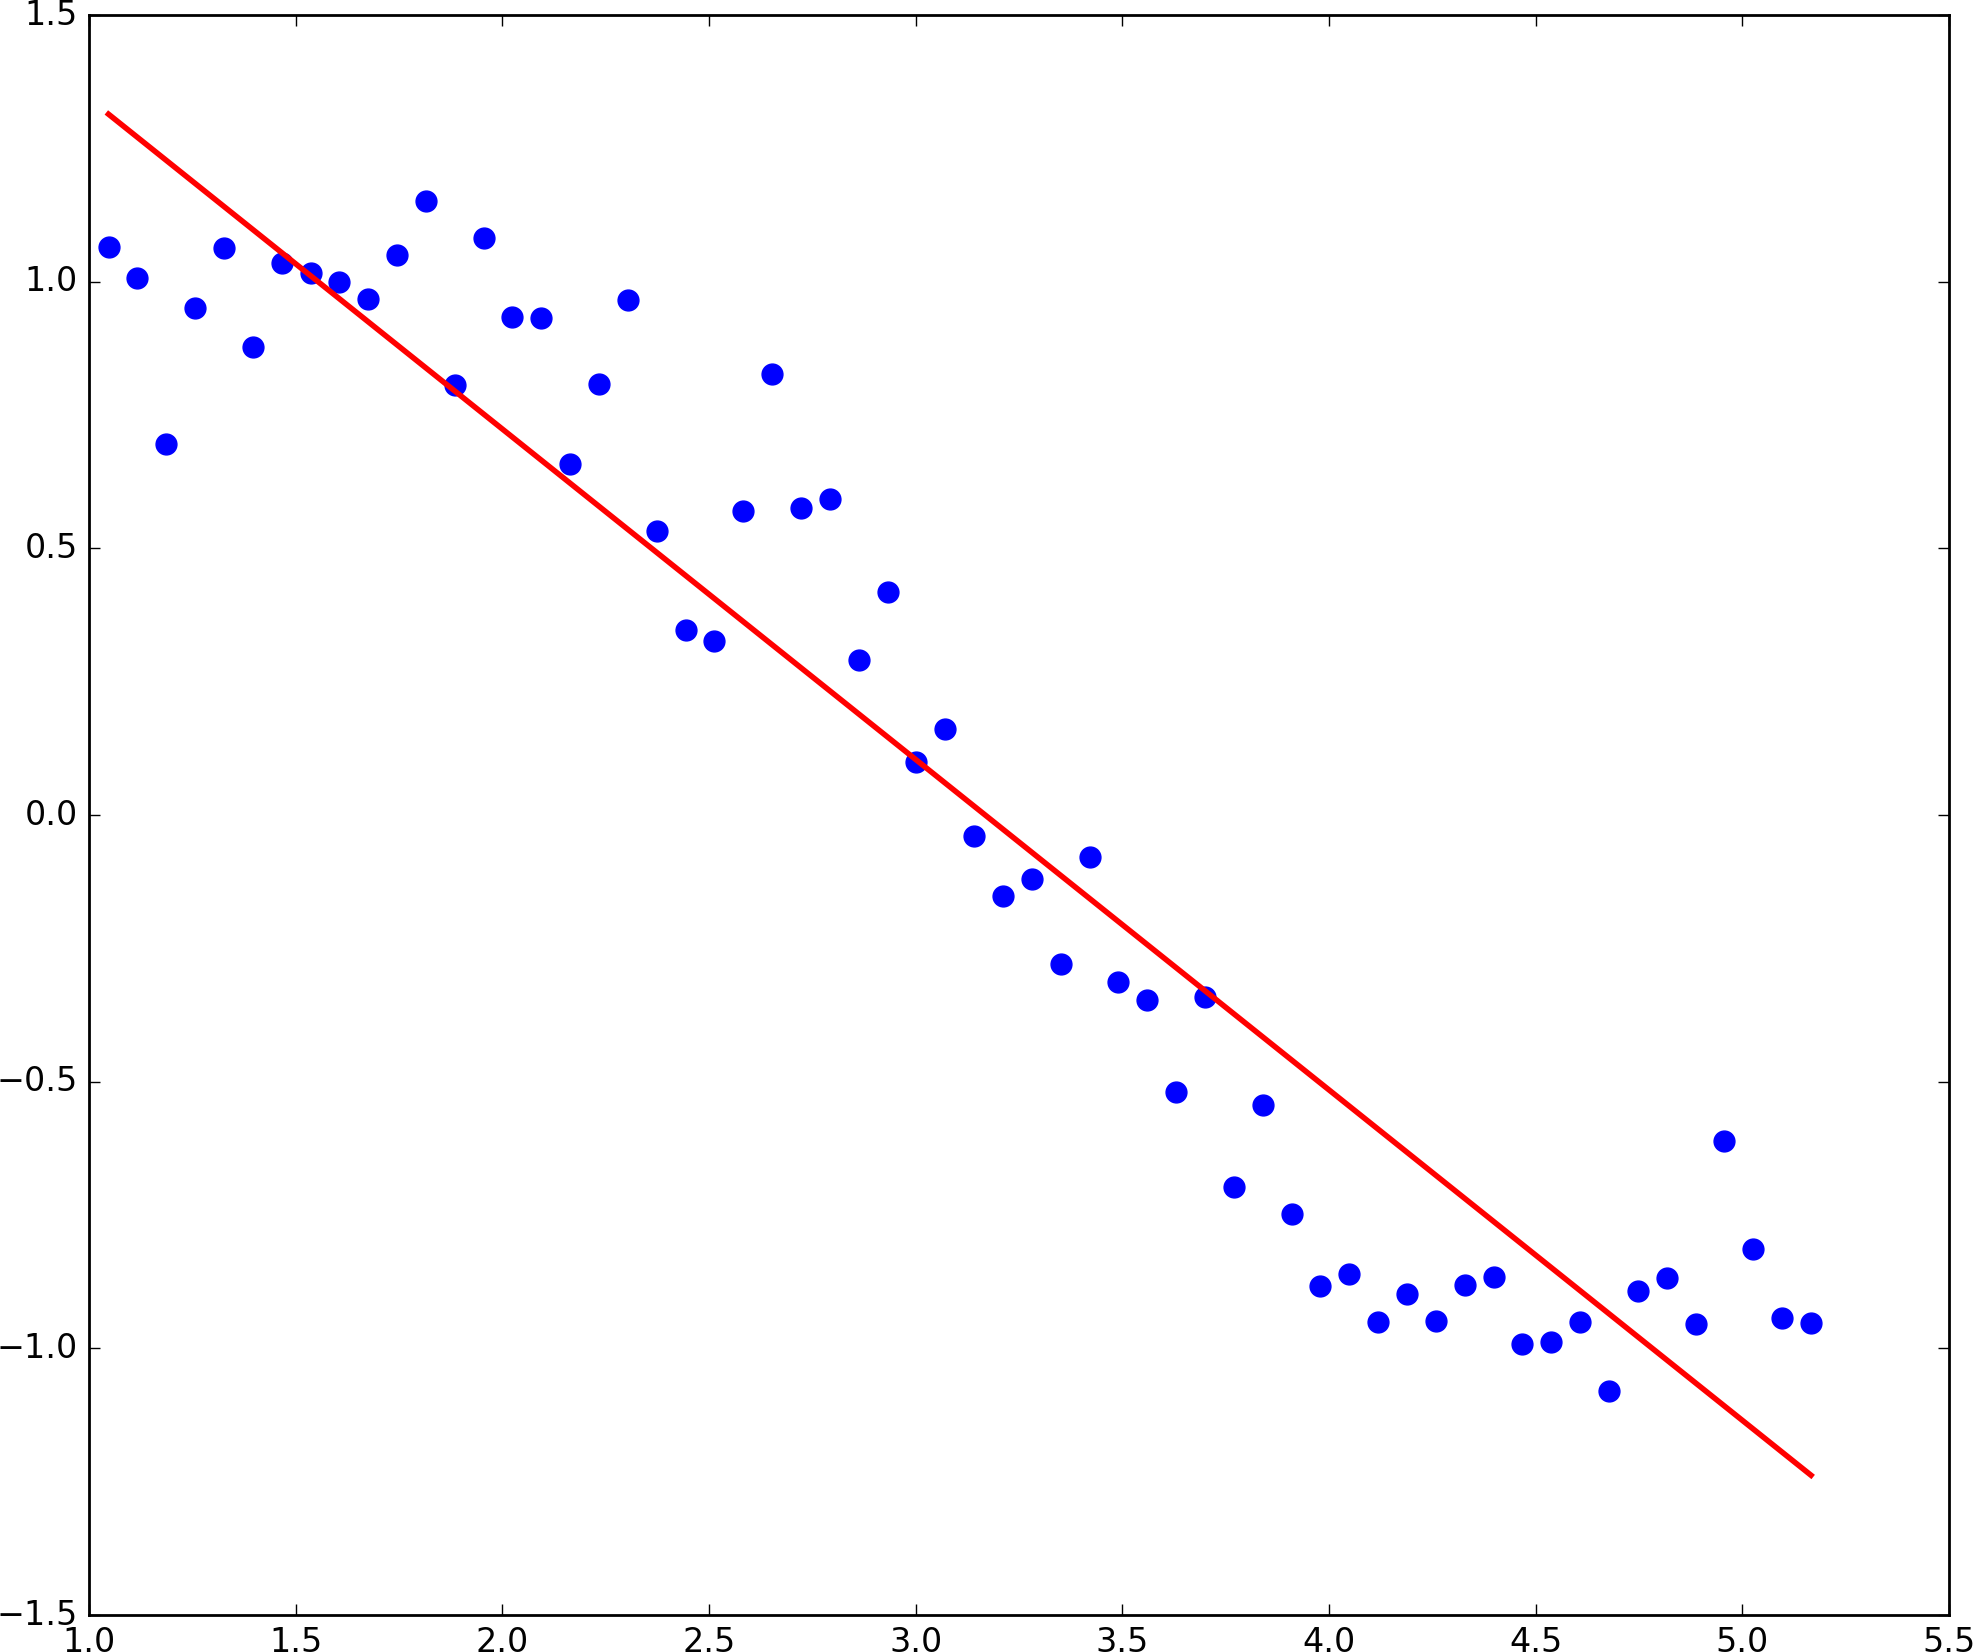
\includegraphics[width=0.99\textwidth]{./fig/L1/linreg_pow1.png}
\end{figure}
\column{.5\textwidth}
\begin{figure}
residuals\\
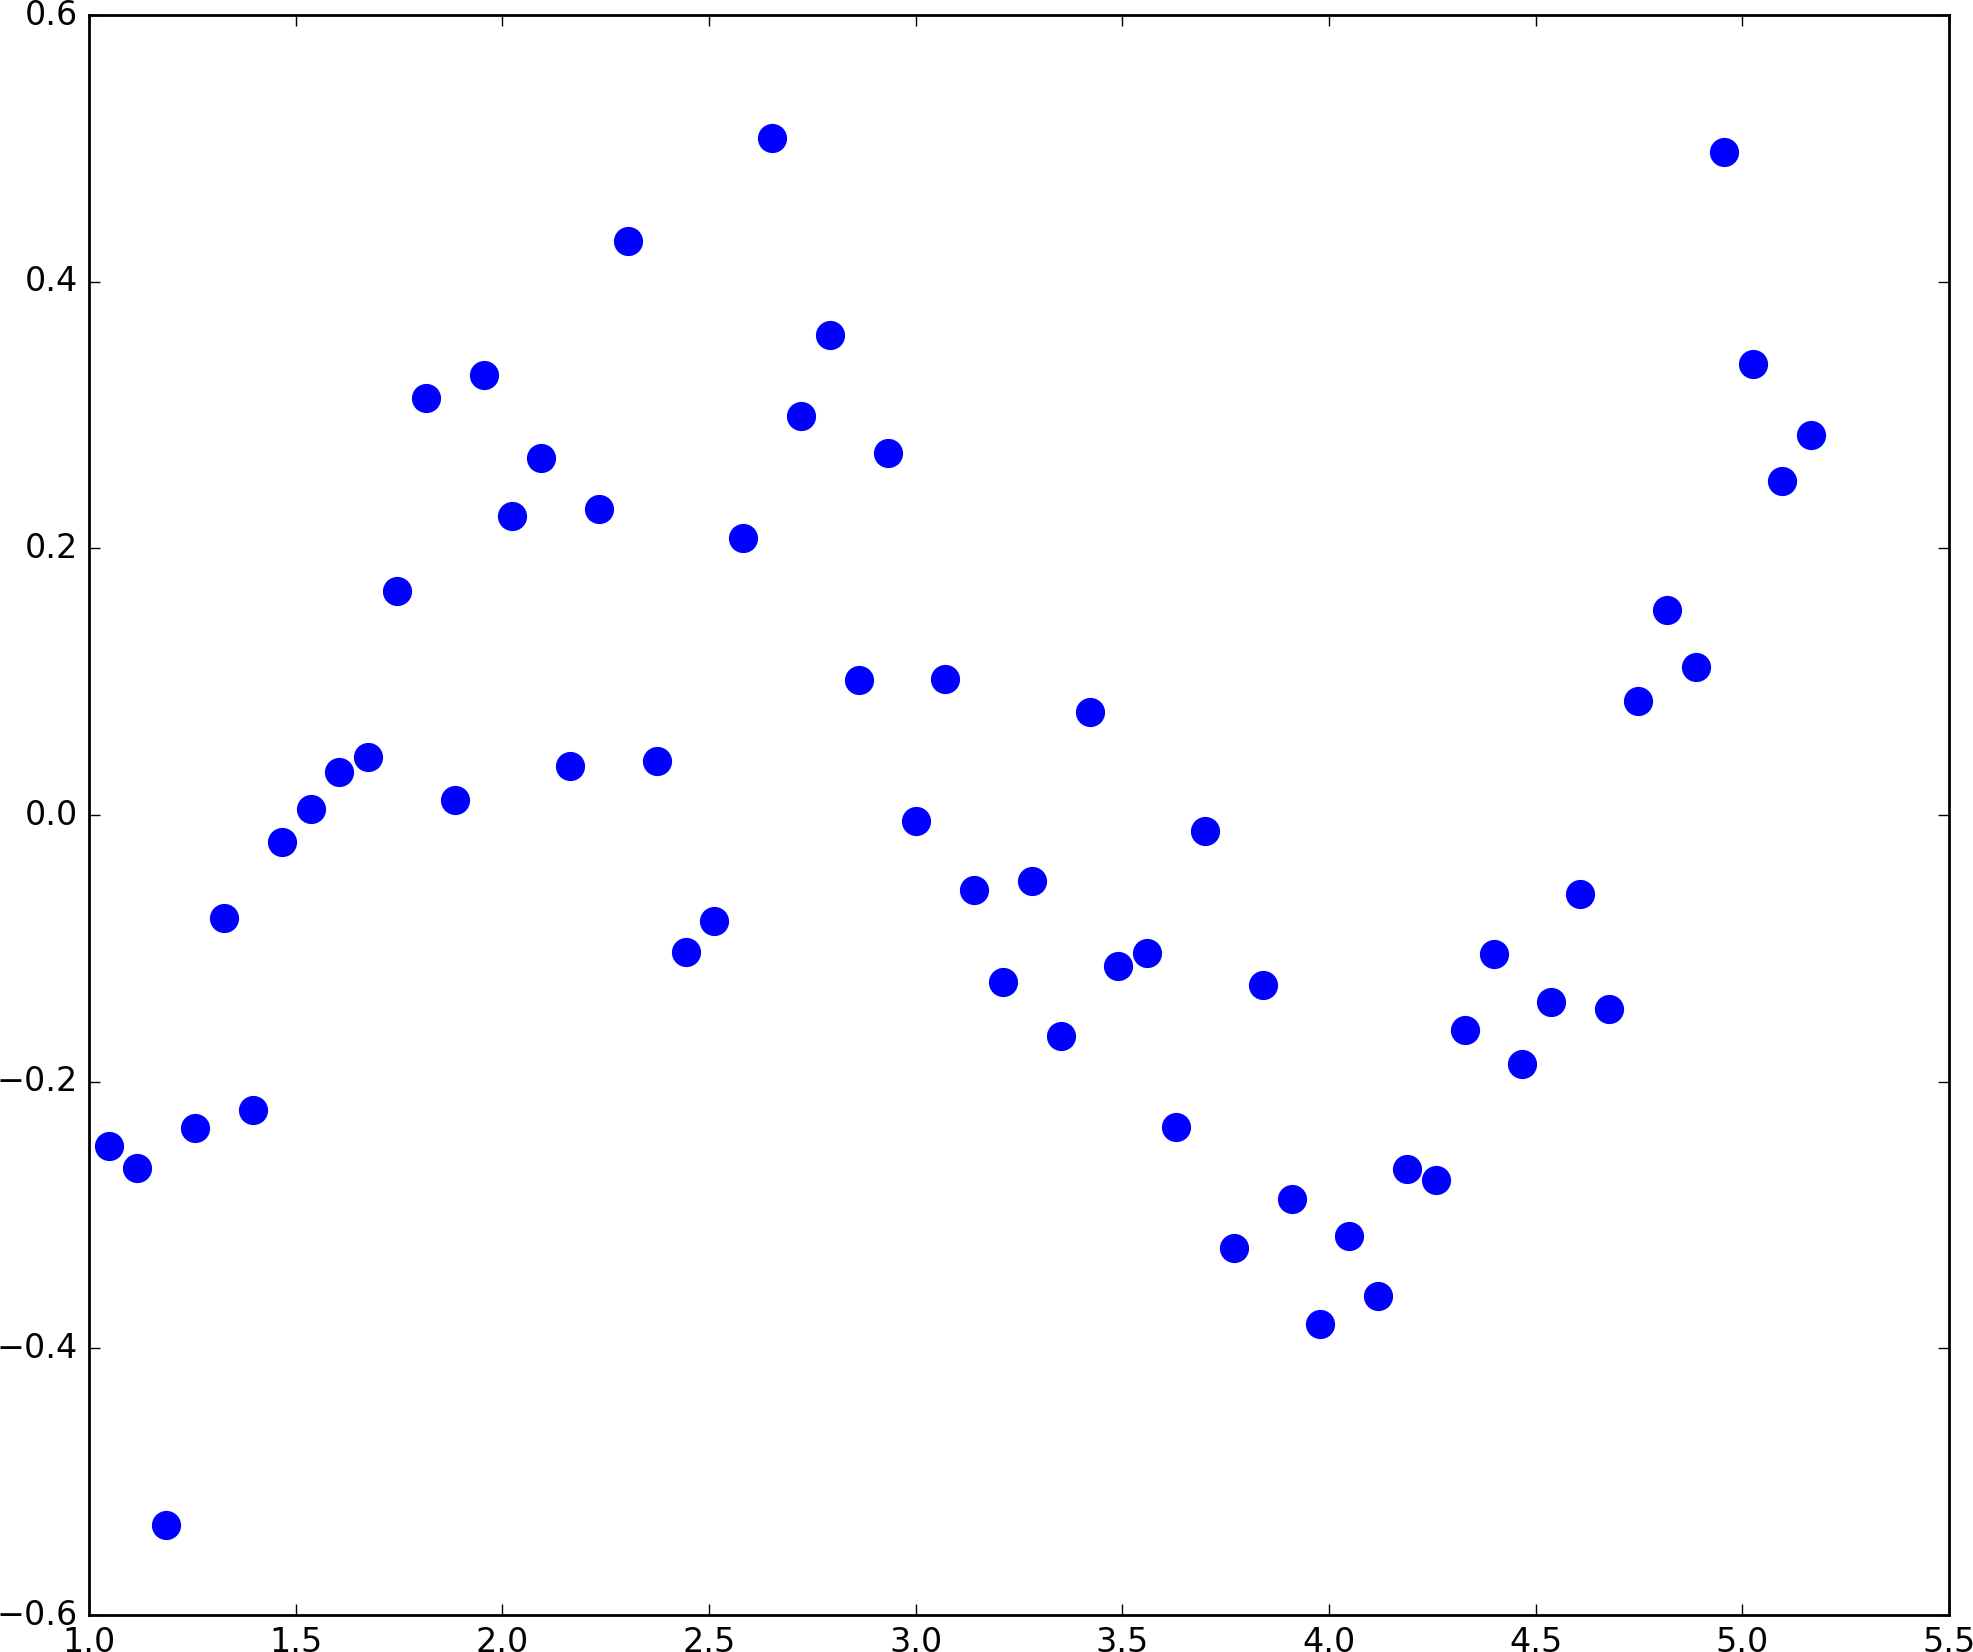
\includegraphics[width=0.99\textwidth]{./fig/L1/residuals.png}
\end{figure}

\end{columns}
\begin{block}{Prediction error}
$$
\text{err} = \frac{1}{n}\sum \text{res}^2 = 5.46e-2
$$
\end{block}

\end{frame}
%%%%%%%%%%%%%%%%%%%%%
\begin{frame}
\frametitle{Increasing the polynomial degree ?}
\begin{columns}
\column{.5\textwidth}
\begin{figure}
$p=3$ (cubic regression)\\
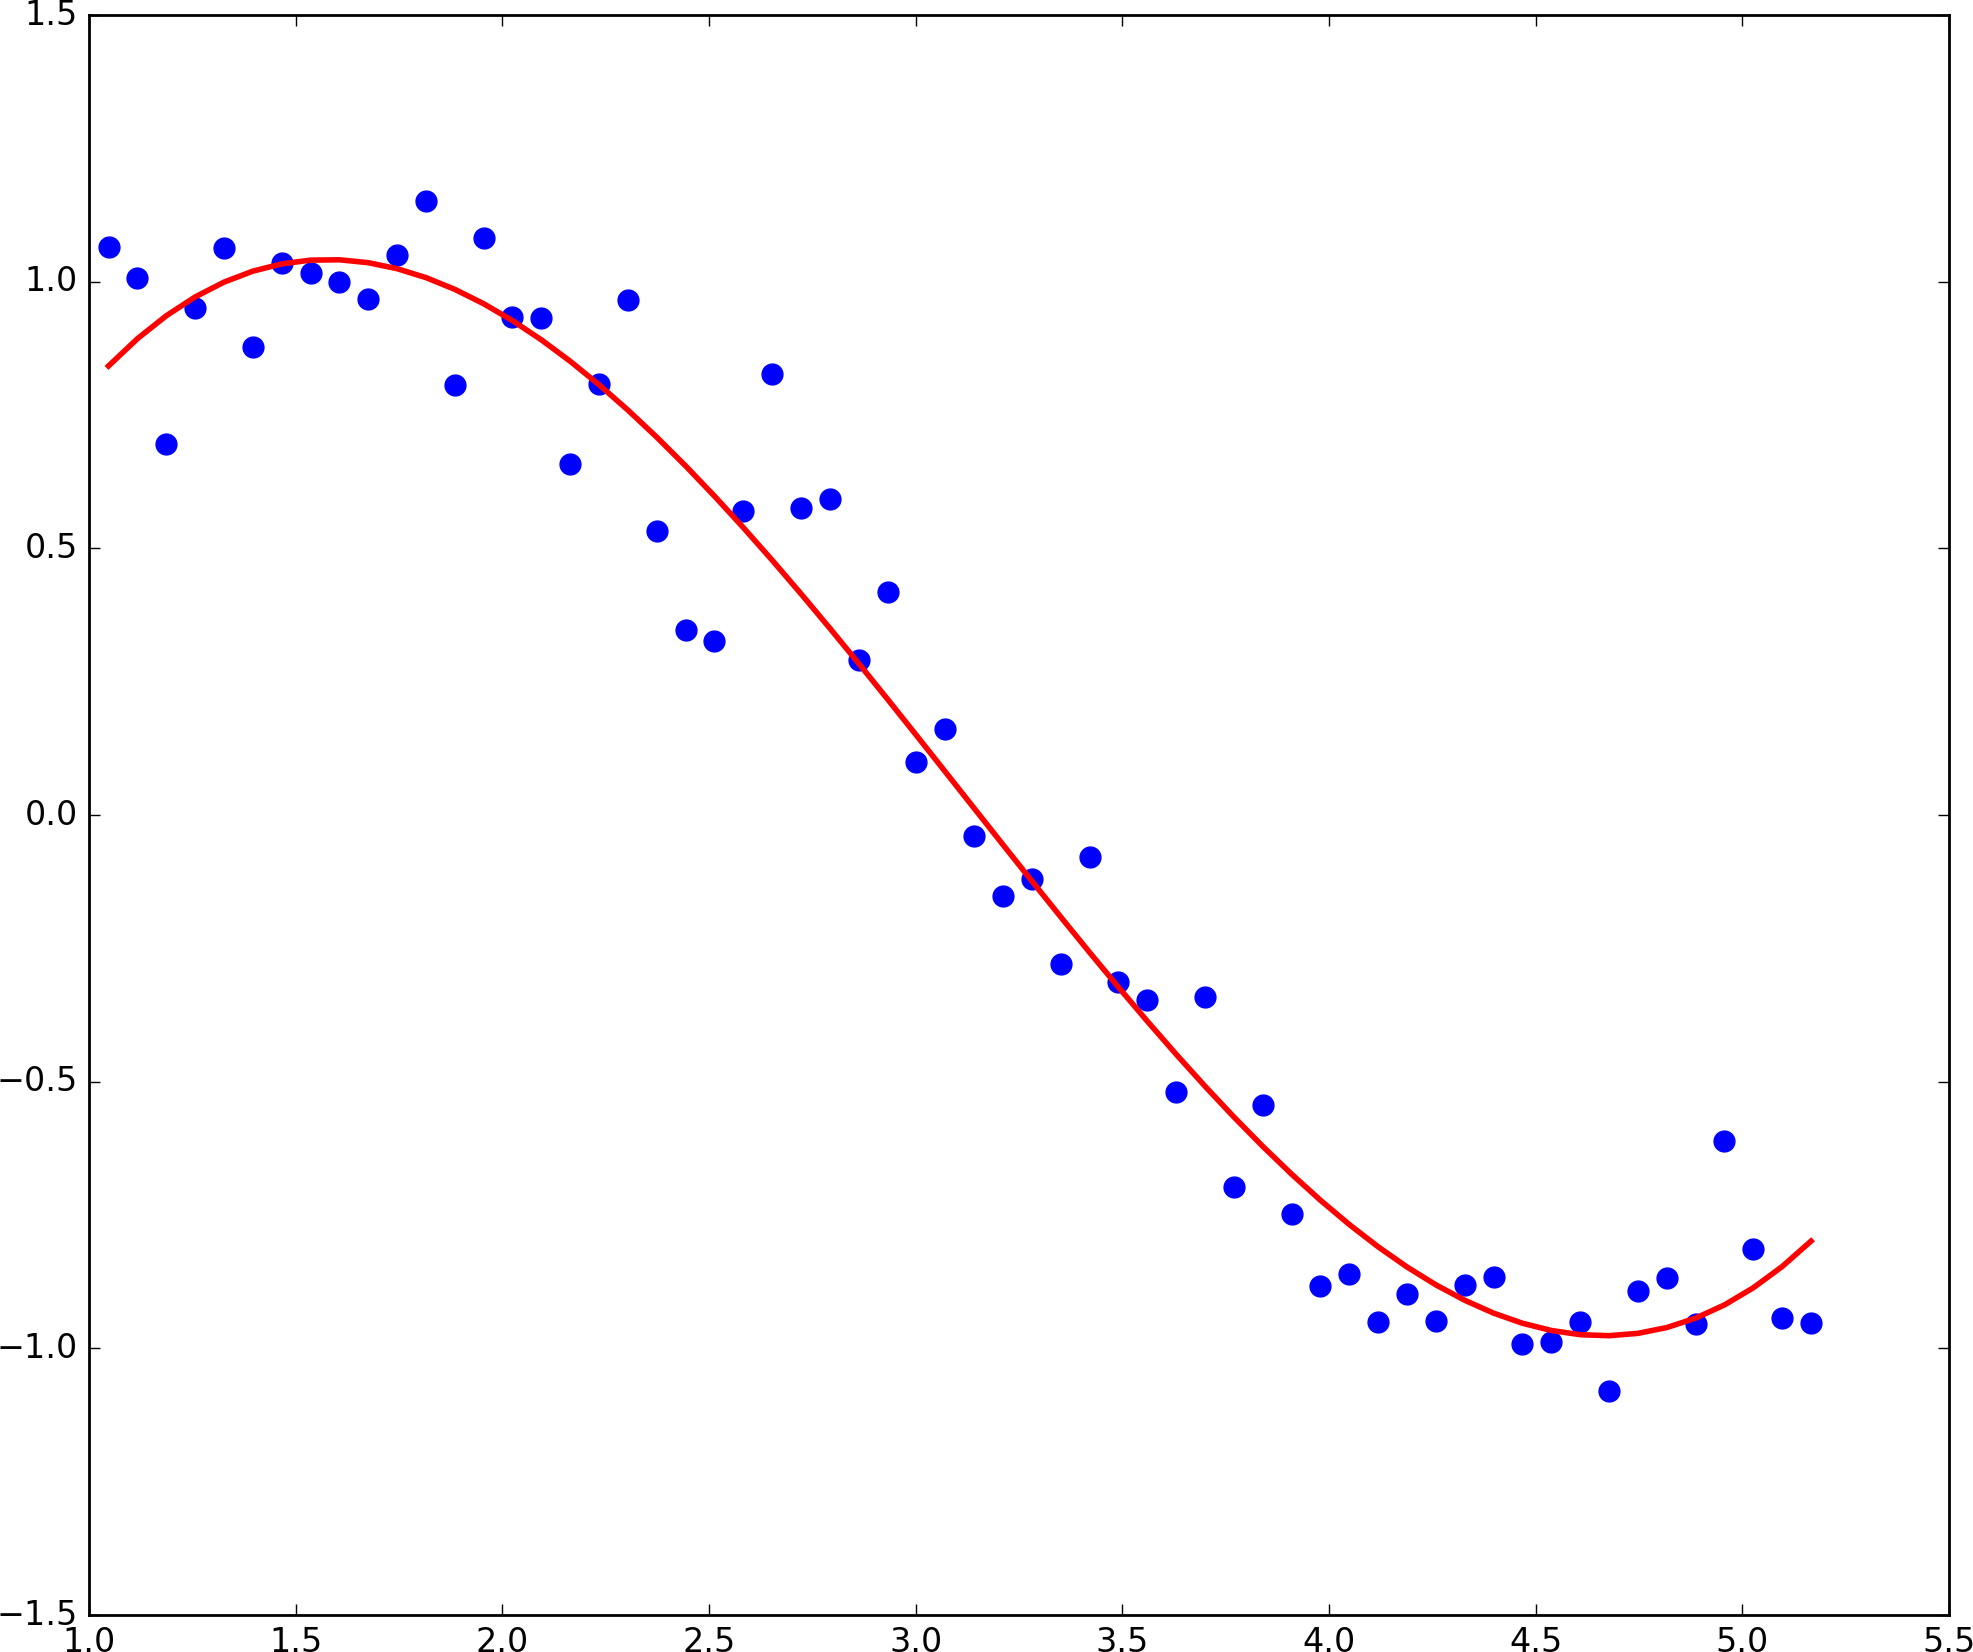
\includegraphics[width=0.99\textwidth]{./fig/L1/linreg_pow3.png}
\end{figure}
\column{.5\textwidth}
\begin{block}{Prediction error}
$$
\text{err} = \frac{1}{n}\sum \text{res}^2 = 1.80e-2
$$
\end{block}
\end{columns}
\end{frame}


%%%%%%%%%%%%%%%%%%%%%
\begin{frame}
\frametitle{Is it different from the linear regression ?}
Let's consider :
$$
\bm{x} = 
\begin{pmatrix}
1 \\
x^1 \\
x^2 \\
\vdots \\
x^p
\end{pmatrix}
$$
then
$$
h_{\bm{\theta}}(x) = \theta_0  + \theta_1 x^1 + \ldots + \theta_p x^p = \bm{\theta}^T \bm{x}
$$
\begin{alertblock}{}
By extending a scalar predictor to a vector,
polynomial regression is equivalent to linear regression.
\end{alertblock}

\end{frame}

%%%%%%%%%%%%%%%%%%%%%
\begin{frame}
\frametitle{Increasing the degree ?}
\begin{columns}
\column{.33\textwidth}
\vspace{-2em}
\begin{figure}
$p=1$
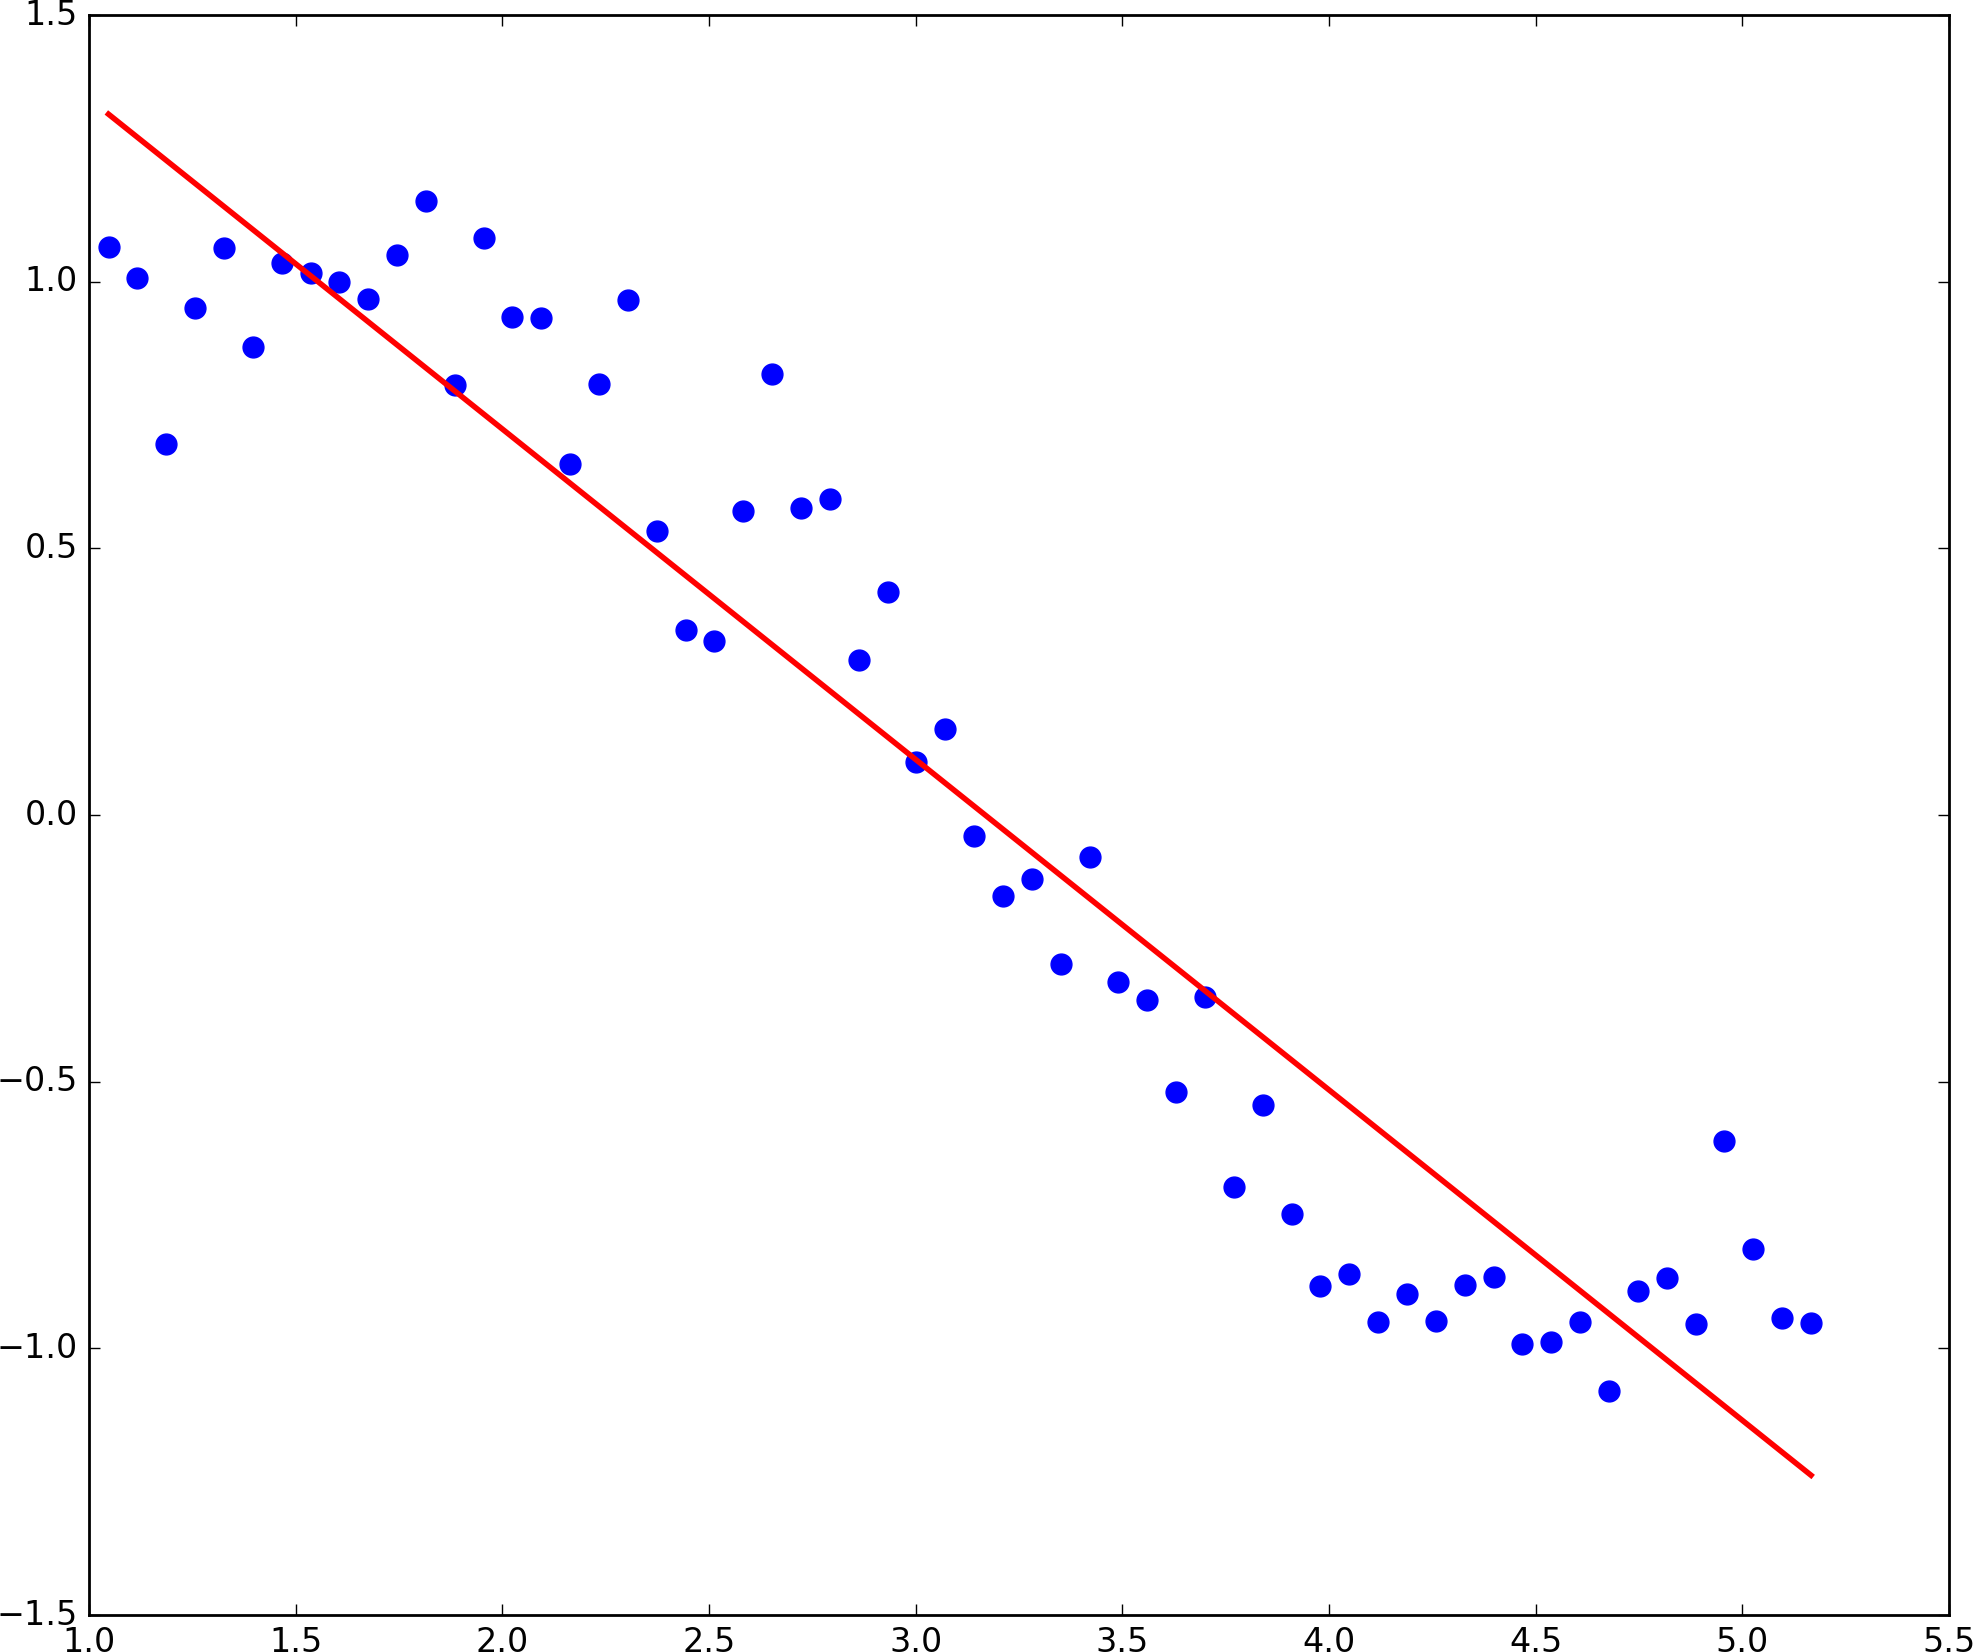
\includegraphics[width=0.99\textwidth]{./fig/L1/linreg_pow1.png}
\end{figure}
\vspace{-2em}
\begin{figure}
$p=9$
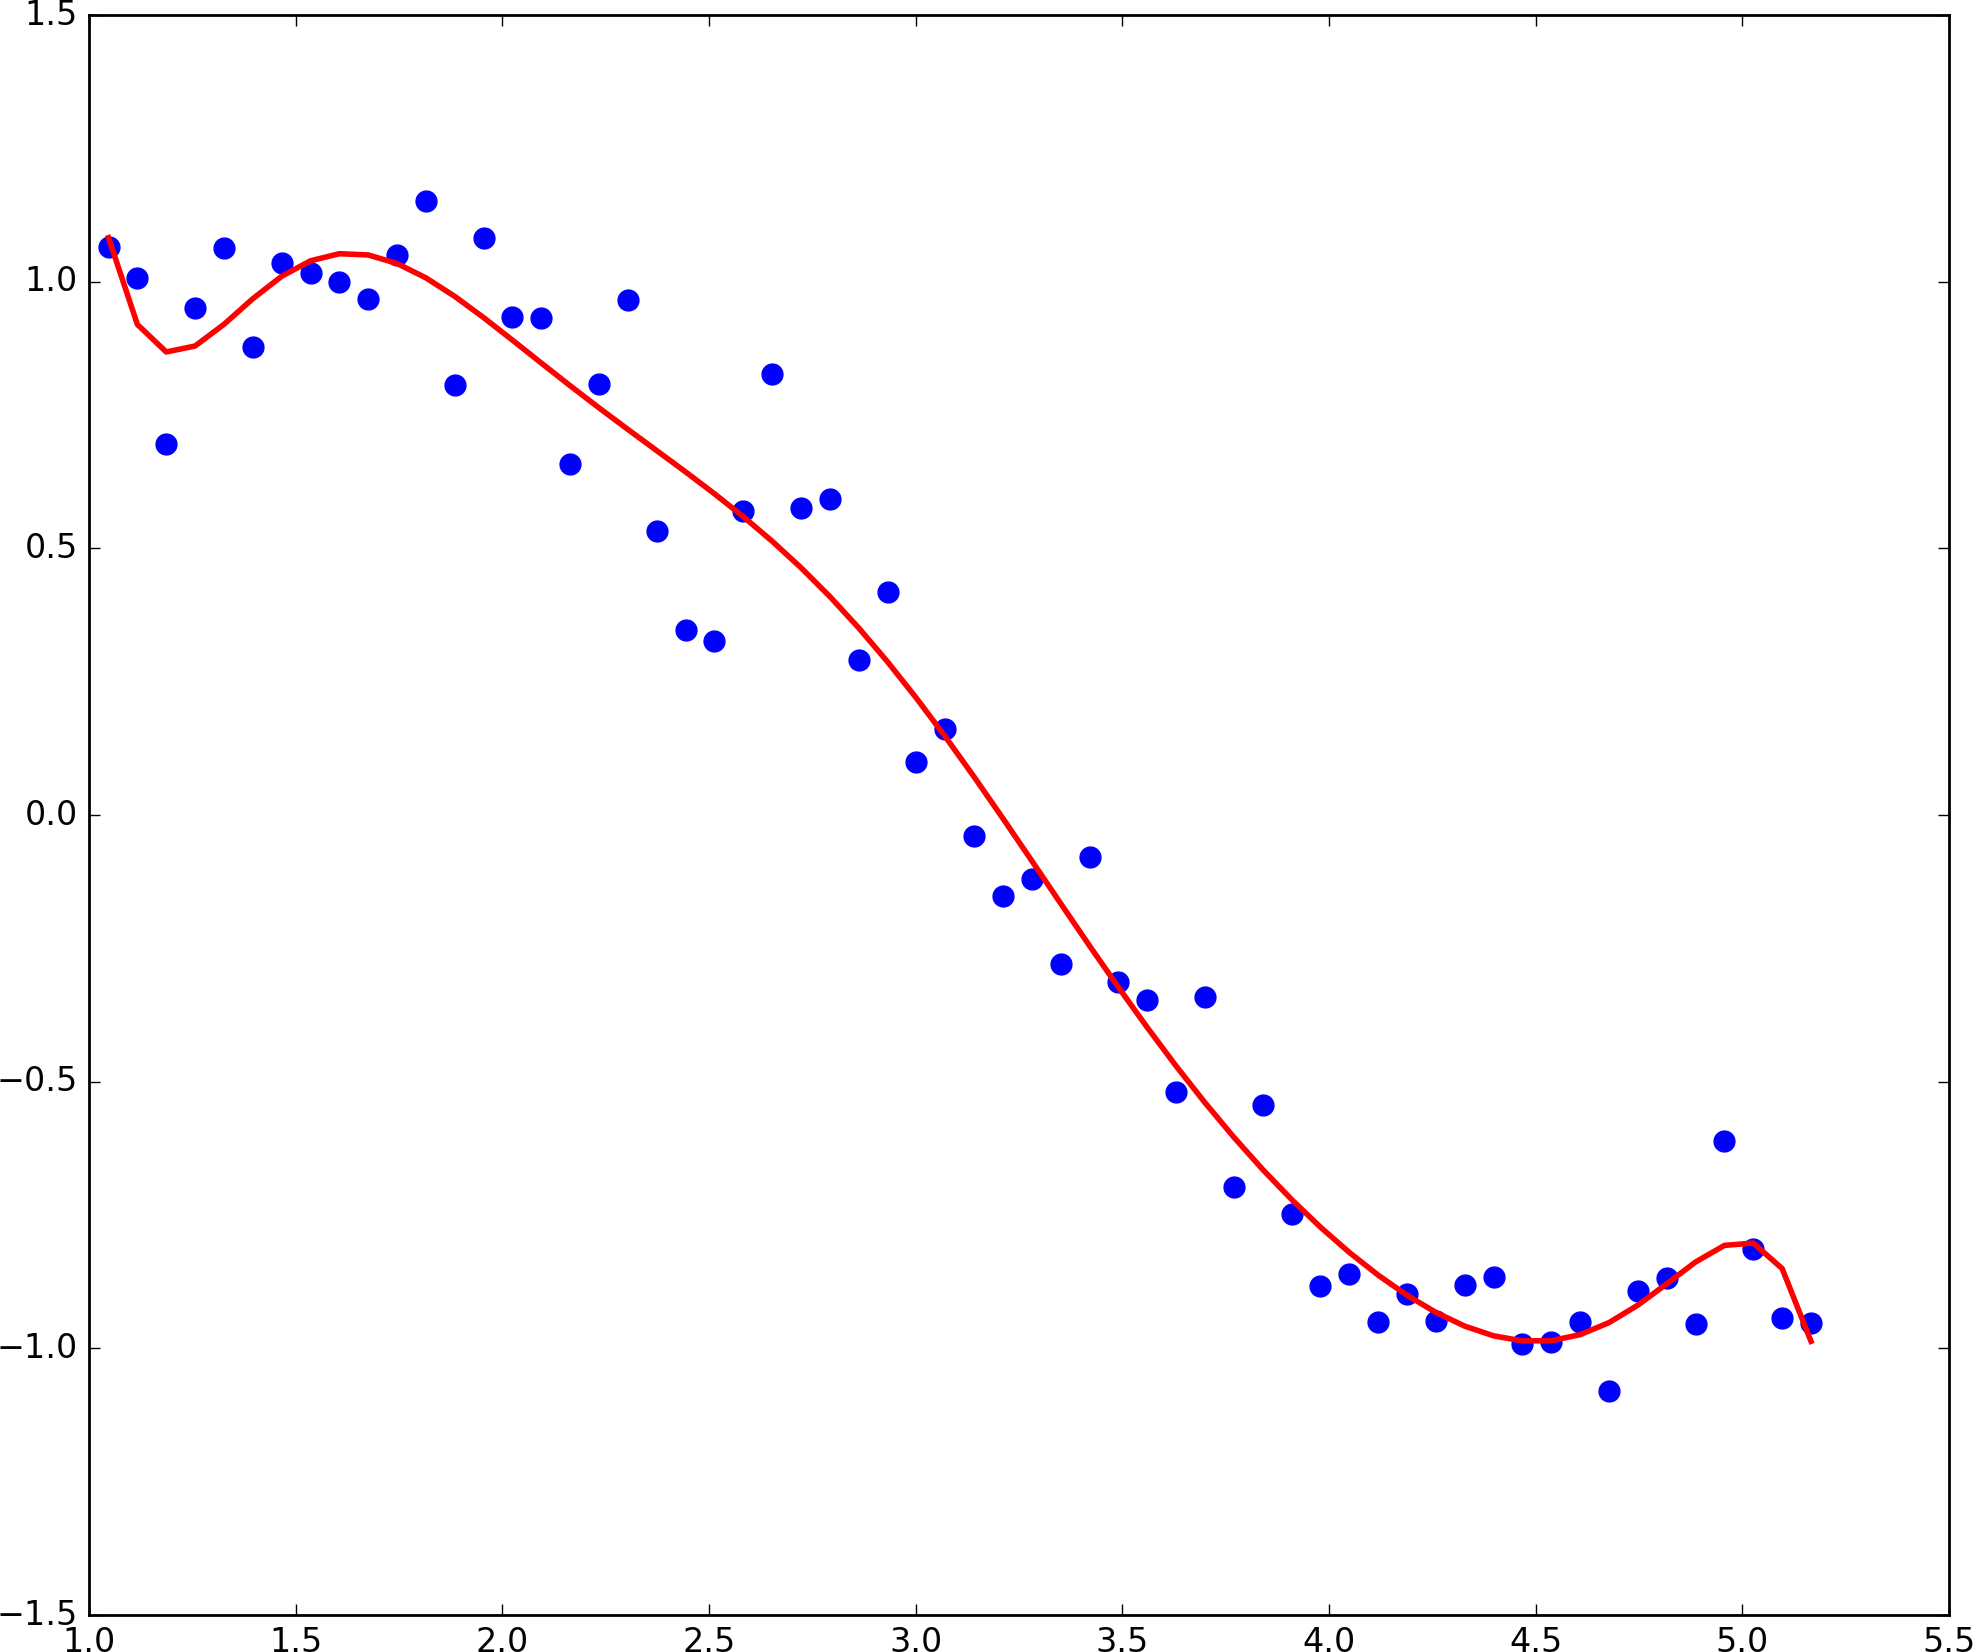
\includegraphics[width=0.99\textwidth]{./fig/L1/linreg_pow9.png}
\end{figure}
\column{.33\textwidth}
\vspace{-2em}
\begin{figure}
$p=3$
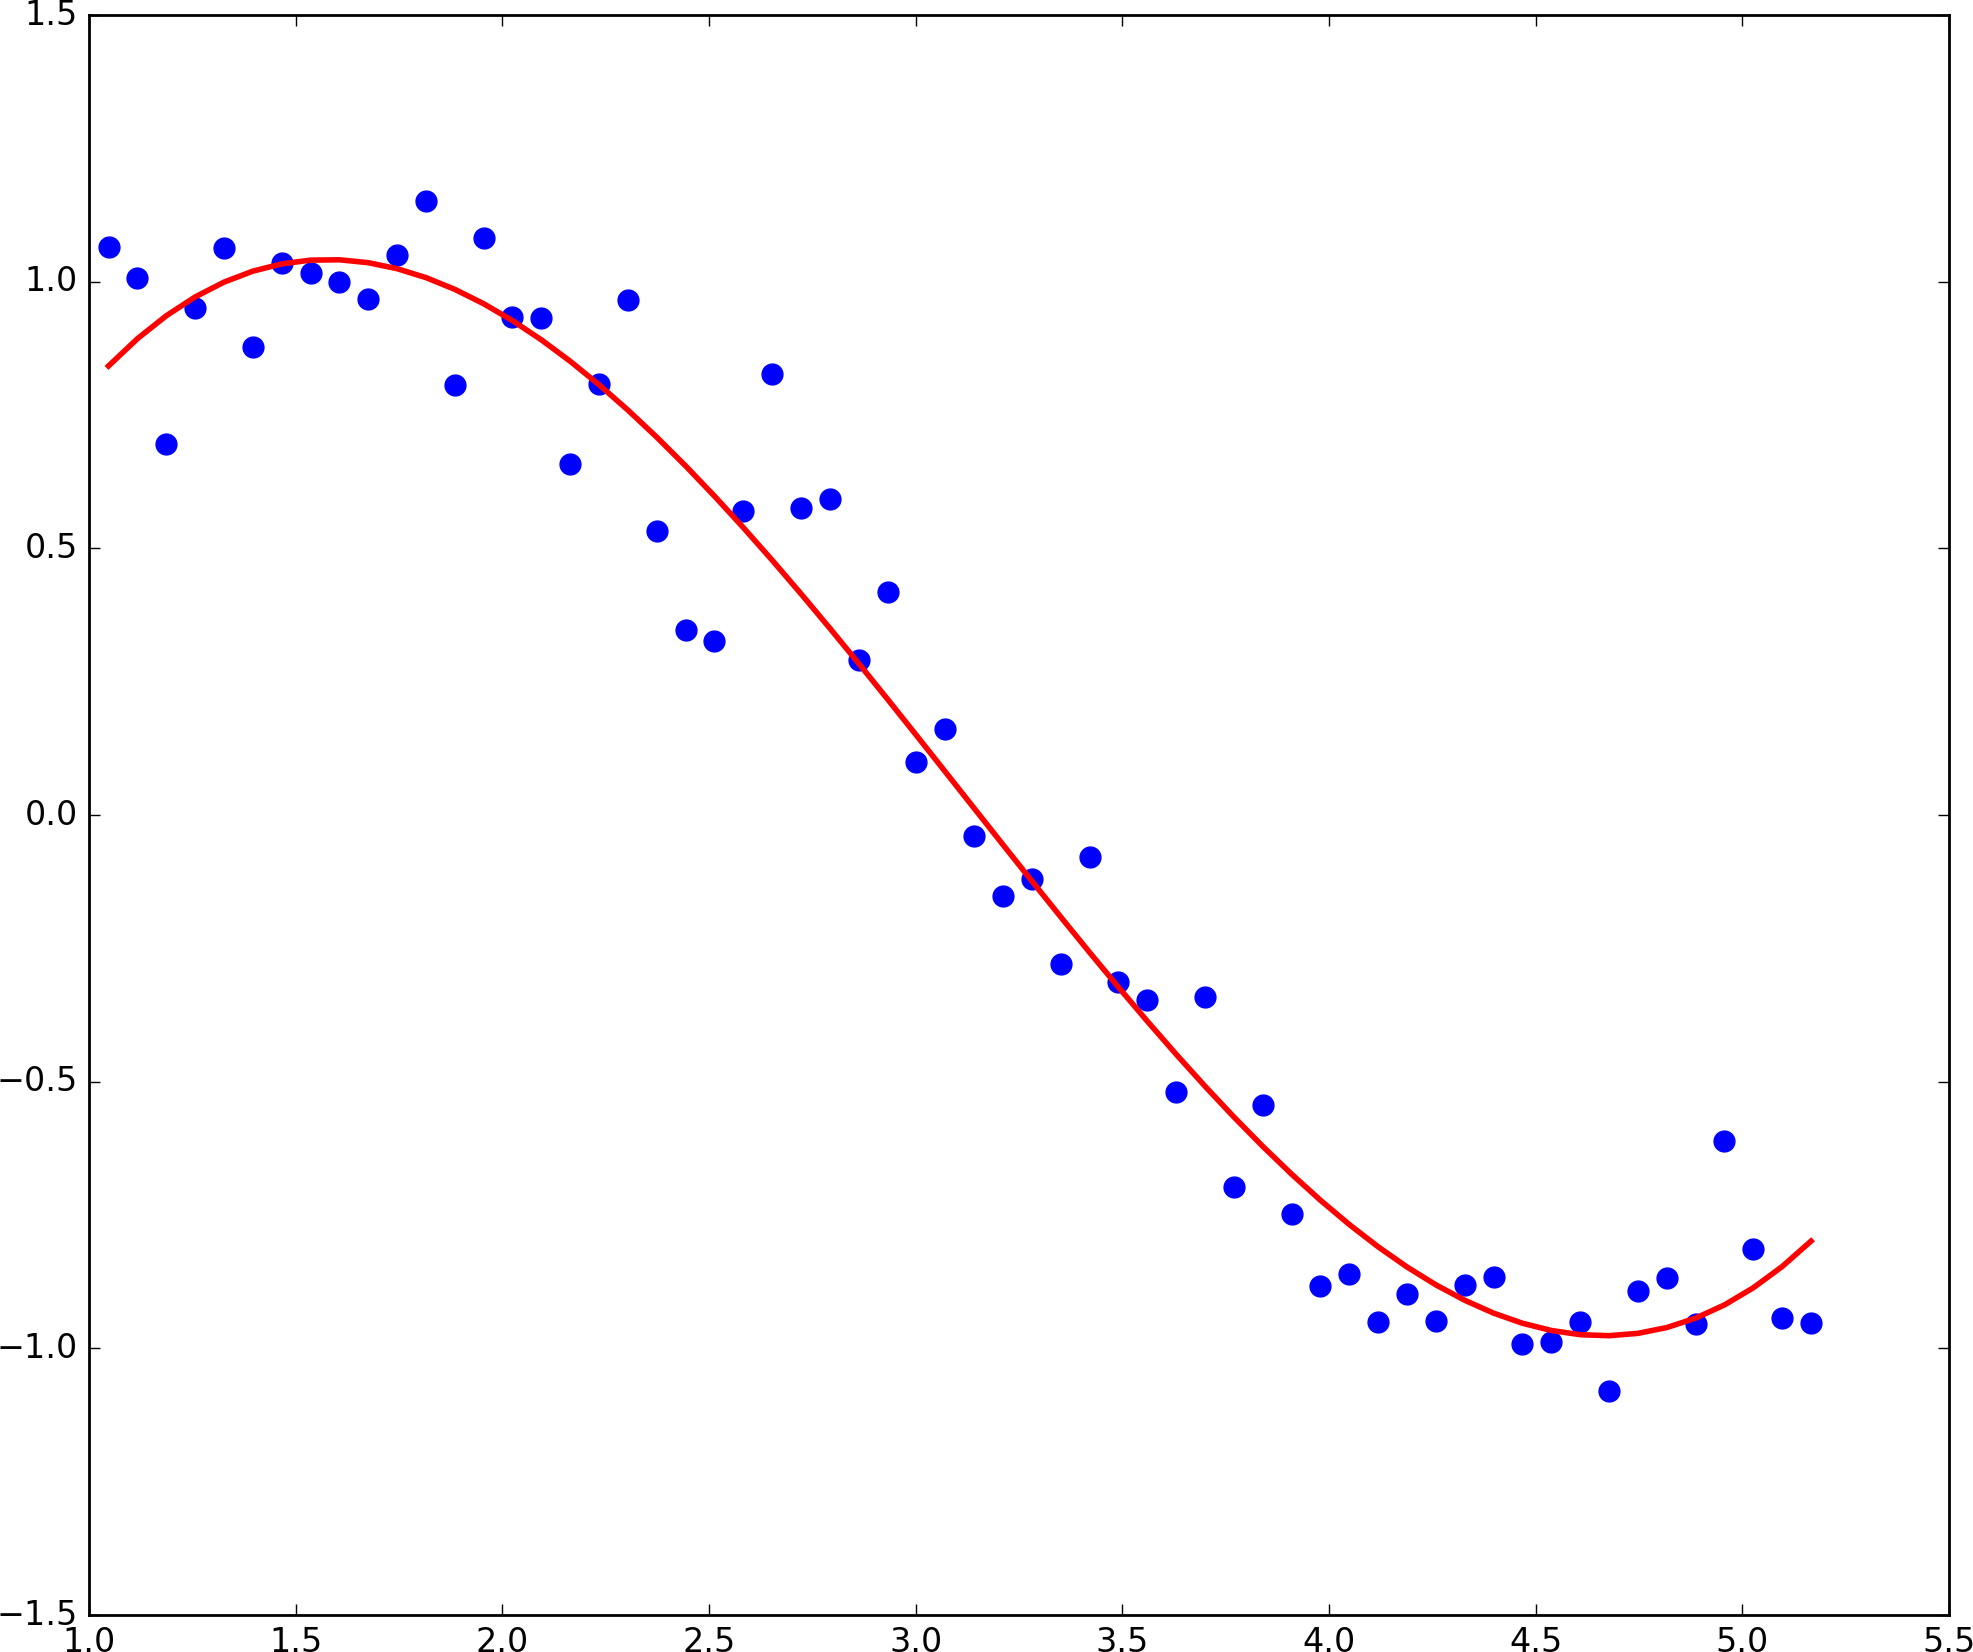
\includegraphics[width=0.99\textwidth]{./fig/L1/linreg_pow3.png}
\end{figure}
\vspace{-2em}
\begin{figure}
$p=12$
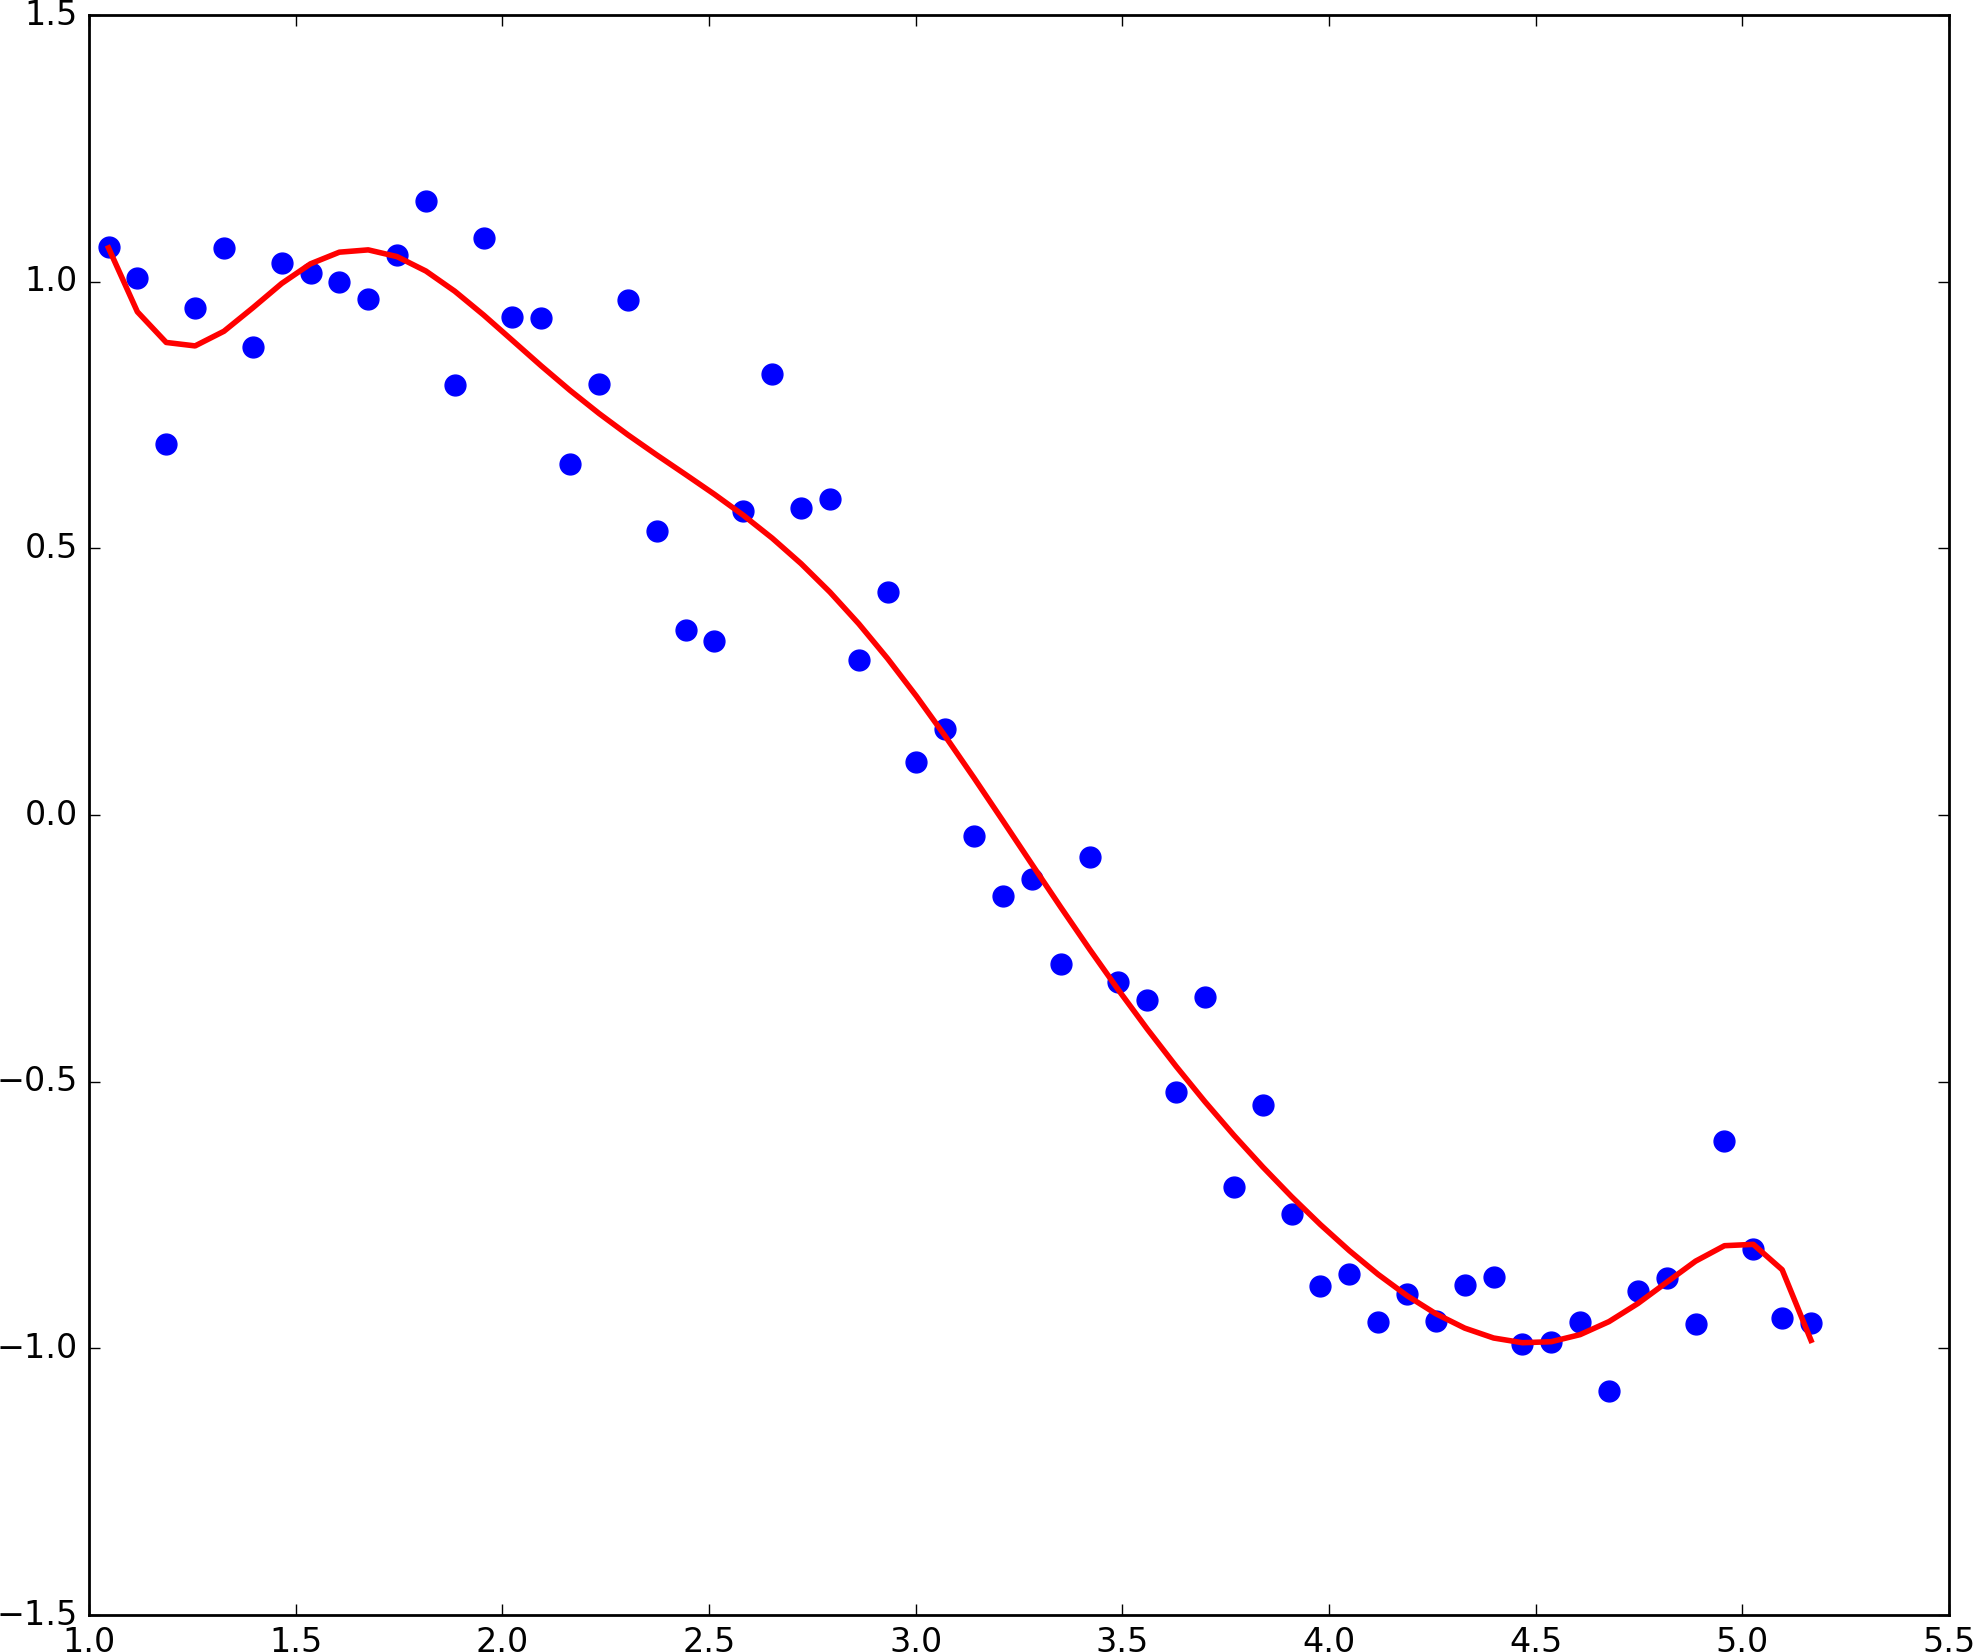
\includegraphics[width=0.99\textwidth]{./fig/L1/linreg_pow12.png}
\end{figure}
\column{.33\textwidth}
\vspace{-2em}
\begin{figure}
$p=4$
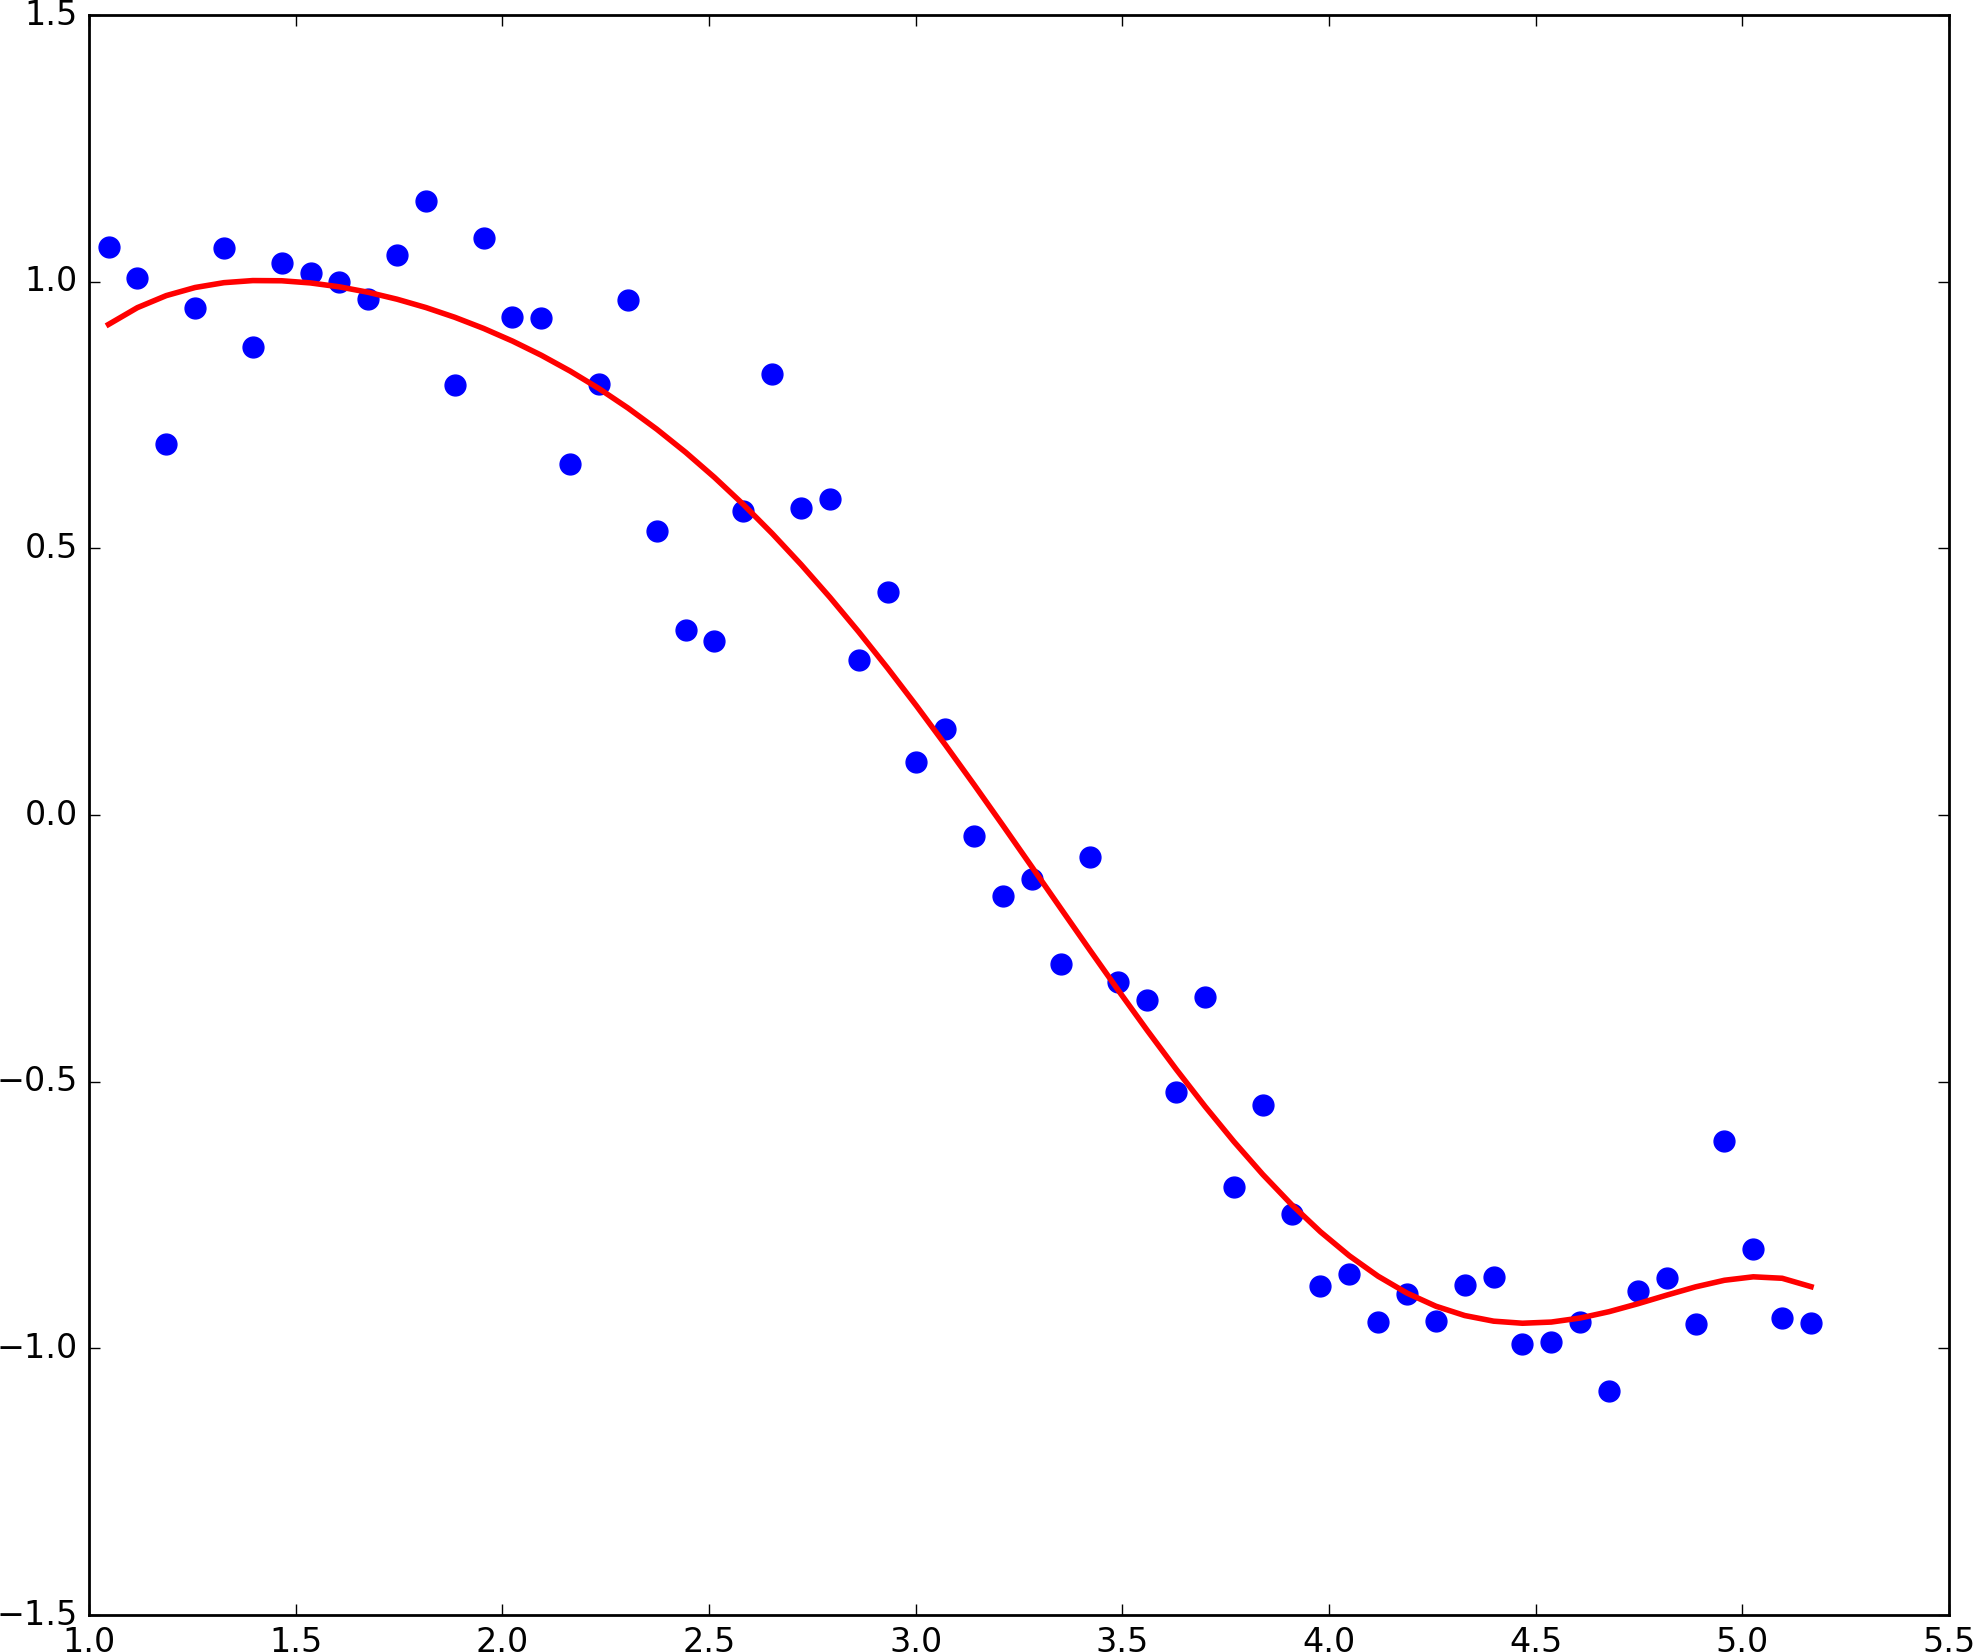
\includegraphics[width=0.99\textwidth]{./fig/L1/linreg_pow4.png}
\end{figure}
\vspace{-2em}
\begin{figure}
$p=15$
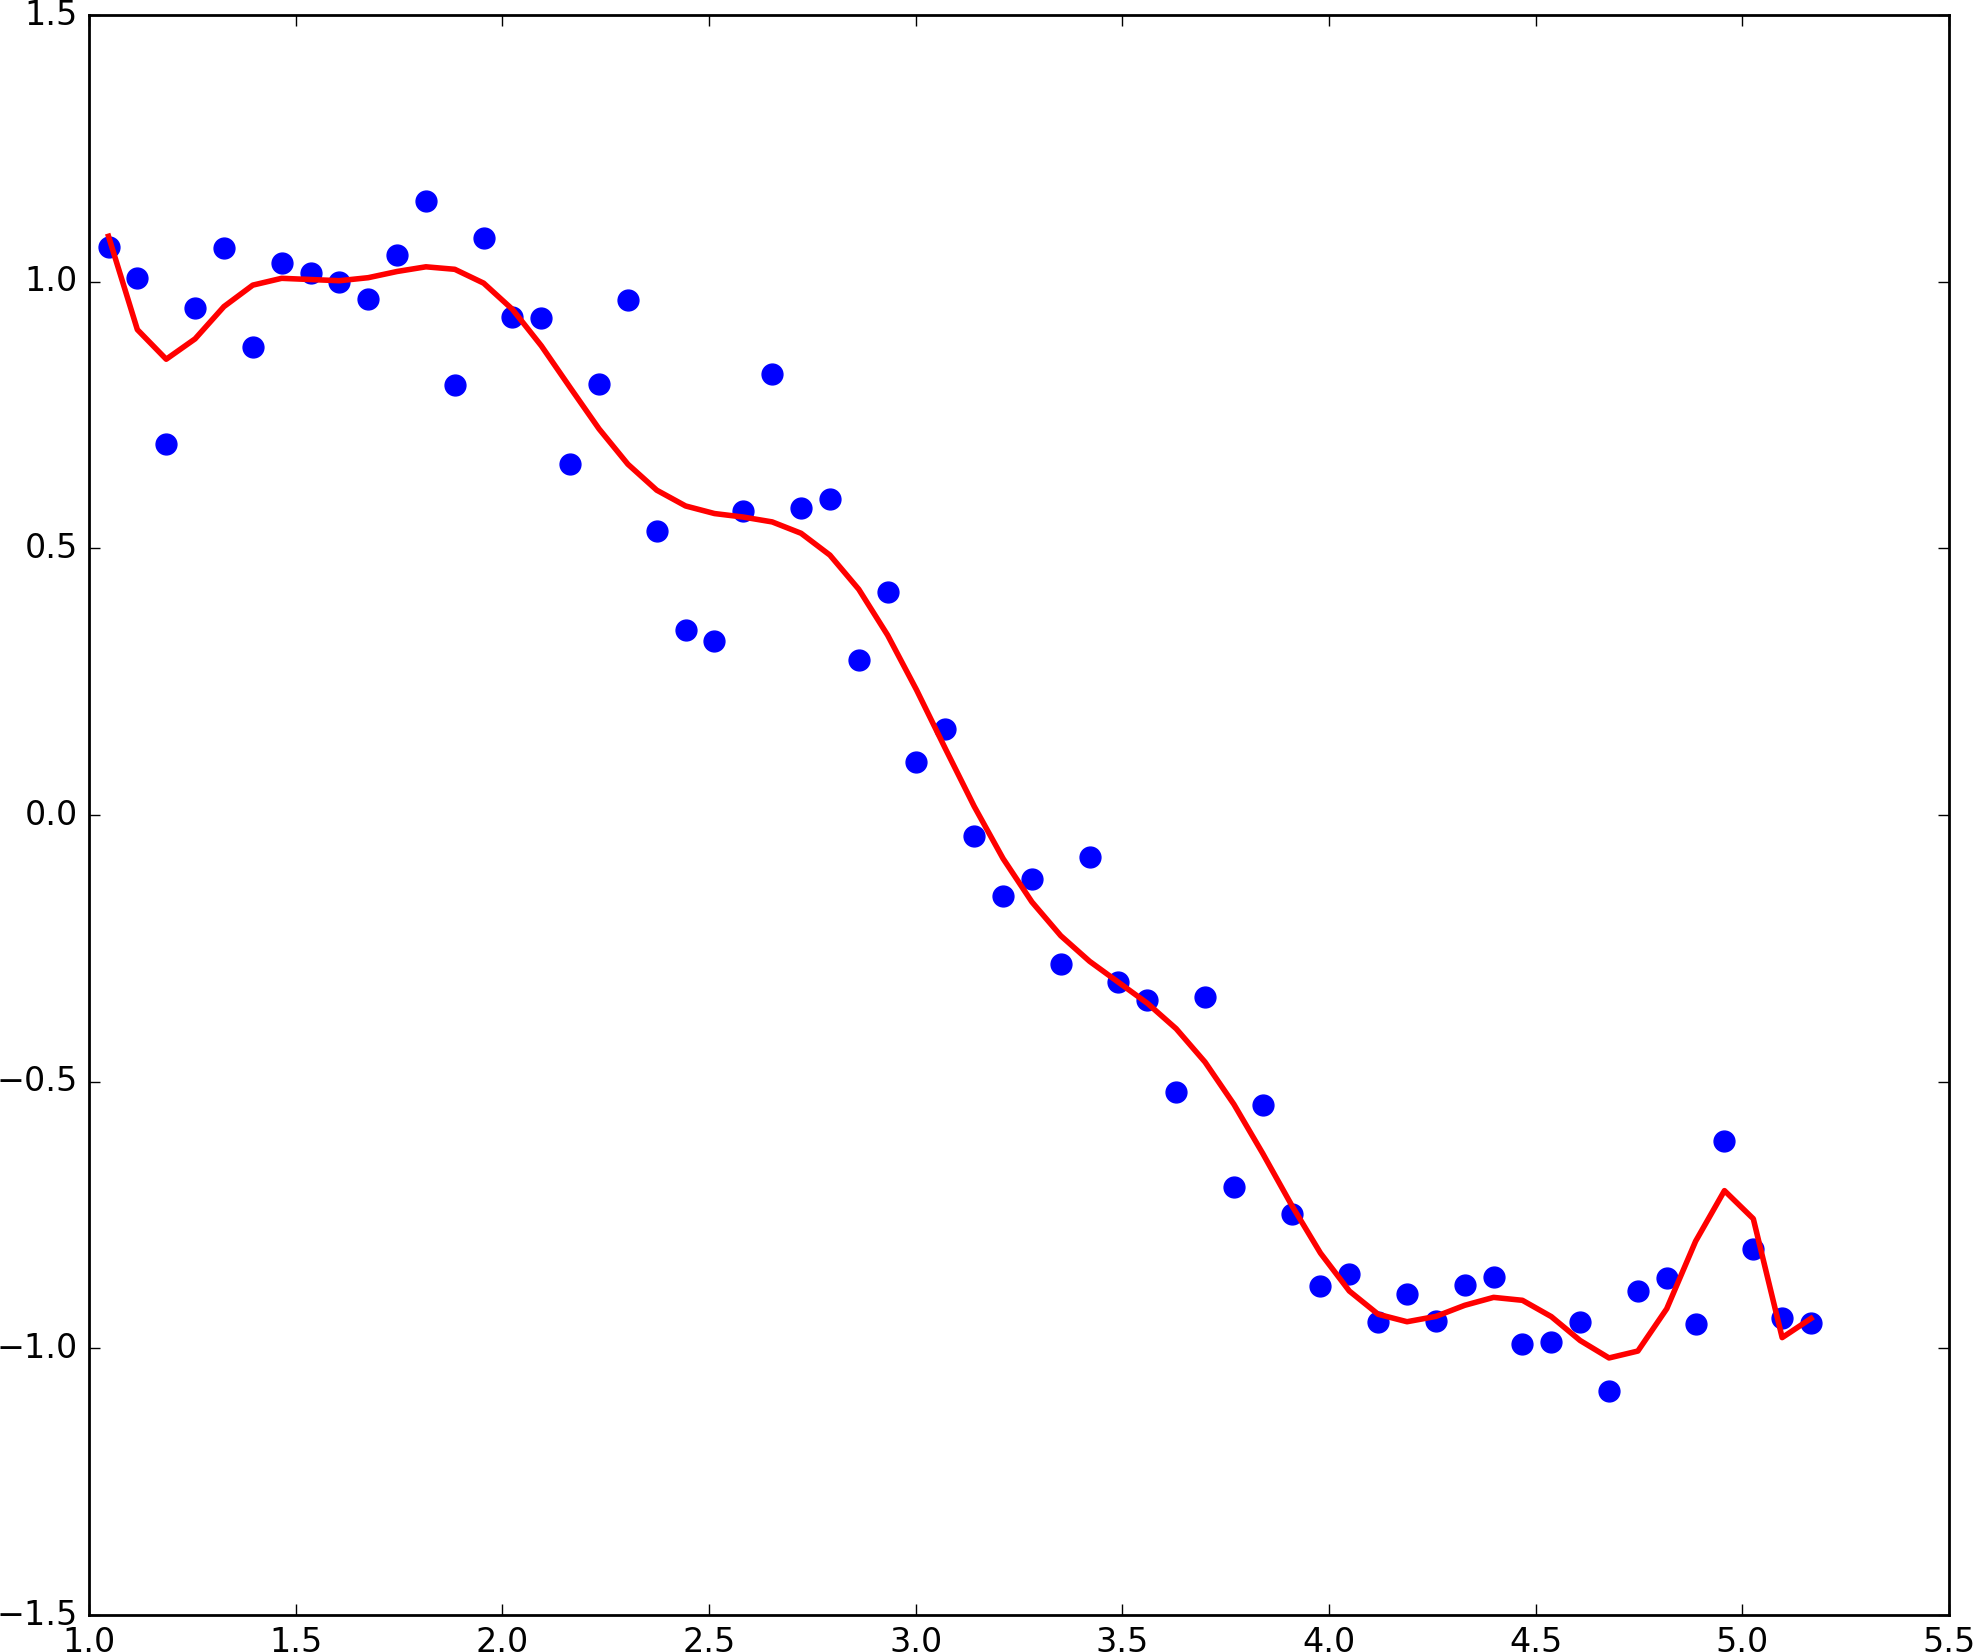
\includegraphics[width=0.99\textwidth]{./fig/L1/linreg_pow15.png}
\end{figure}
\end{columns}
\end{frame}


%%%%%%%%%%%%%%%%%%%%%
\begin{frame}
\frametitle{Overfitting}
\begin{block}{}
When there is to many paramaters to fit, the model can reproduce 
a random noise, it is called \alert{overfitting}
\end{block}
\pause
\begin{table}
\resizebox{\textwidth}{!}{%
\begin{tabular}{lllllllllll}
\toprule
{} &      rmse &      th\_0 &      th\_1 &      th\_2 &      th\_3 &      th\_4 &      th\_5 &      th\_6 &      th\_7 &      th\_8 \\
\midrule
max\_pow\_1  & +5.47e-02 & +1.96e+00 & -6.20e-01 &       NaN &       NaN &       NaN &       NaN &       NaN &       NaN &       NaN \\
max\_pow\_2  & +5.46e-02 & +1.91e+00 & -5.83e-01 & -5.96e-03 &       NaN &       NaN &       NaN &       NaN &       NaN &       NaN \\
max\_pow\_3  & +1.84e-02 & -1.08e+00 & +3.03e+00 & -1.29e+00 & +1.37e-01 &       NaN &       NaN &       NaN &       NaN &       NaN \\
max\_pow\_4  & +1.80e-02 & -2.66e-01 & +1.69e+00 & -5.32e-01 & -3.57e-02 & +1.39e-02 &       NaN &       NaN &       NaN &       NaN \\
max\_pow\_5  & +1.70e-02 & +2.99e+00 & -5.12e+00 & +4.72e+00 & -1.93e+00 & +3.35e-01 & -2.07e-02 &       NaN &       NaN &       NaN \\
max\_pow\_6  & +1.65e-02 & -2.80e+00 & +9.52e+00 & -9.71e+00 & +5.23e+00 & -1.55e+00 & +2.33e-01 & -1.36e-02 &       NaN &       NaN \\
max\_pow\_7  & +1.55e-02 & +1.93e+01 & -5.60e+01 & +6.90e+01 & -4.46e+01 & +1.65e+01 & -3.53e+00 & +4.05e-01 & -1.92e-02 &       NaN \\
max\_pow\_8  & +1.53e-02 & +4.32e+01 & -1.37e+02 & +1.84e+02 & -1.33e+02 & +5.77e+01 & -1.53e+01 & +2.42e+00 & -2.10e-01 & +7.68e-03 \\
max\_pow\_9  & +1.46e-02 & +1.68e+02 & -6.15e+02 & +9.63e+02 & -8.46e+02 & +4.61e+02 & -1.62e+02 & +3.68e+01 & -5.22e+00 & +4.22e-01 \\
max\_pow\_10 & +1.46e-02 & +1.38e+02 & -4.86e+02 & +7.26e+02 & -5.96e+02 & +2.93e+02 & -8.75e+01 & +1.45e+01 & -8.06e-01 & -1.38e-01 \\
max\_pow\_11 & +1.45e-02 & -7.49e+01 & +5.12e+02 & -1.33e+03 & +1.87e+03 & -1.61e+03 & +9.14e+02 & -3.50e+02 & +9.14e+01 & -1.61e+01 \\
max\_pow\_12 & +1.45e-02 & -3.39e+02 & +1.87e+03 & -4.42e+03 & +6.01e+03 & -5.25e+03 & +3.12e+03 & -1.30e+03 & +3.84e+02 & -8.03e+01 \\
max\_pow\_13 & +1.43e-02 & +3.20e+03 & -1.78e+04 & +4.46e+04 & -6.66e+04 & +6.61e+04 & -4.61e+04 & +2.32e+04 & -8.55e+03 & +2.30e+03 \\
max\_pow\_14 & +1.31e-02 & +2.38e+04 & -1.41e+05 & +3.79e+05 & -6.10e+05 & +6.57e+05 & -5.03e+05 & +2.82e+05 & -1.17e+05 & +3.66e+04 \\
max\_pow\_15 & +1.17e-02 & -3.62e+04 & +2.44e+05 & -7.46e+05 & +1.38e+06 & -1.71e+06 & +1.53e+06 & -1.00e+06 & +4.98e+05 & -1.88e+05 \\
\bottomrule
\end{tabular}
}
\end{table}
\end{frame}


%%%%%%%%%%%%%%%%%%%%%%%
\begin{frame}
\frametitle{High parameters values}
\begin{figure}
Value of the parameters $|\theta_1|$ with respect with the degree of the polynomial
regression\\
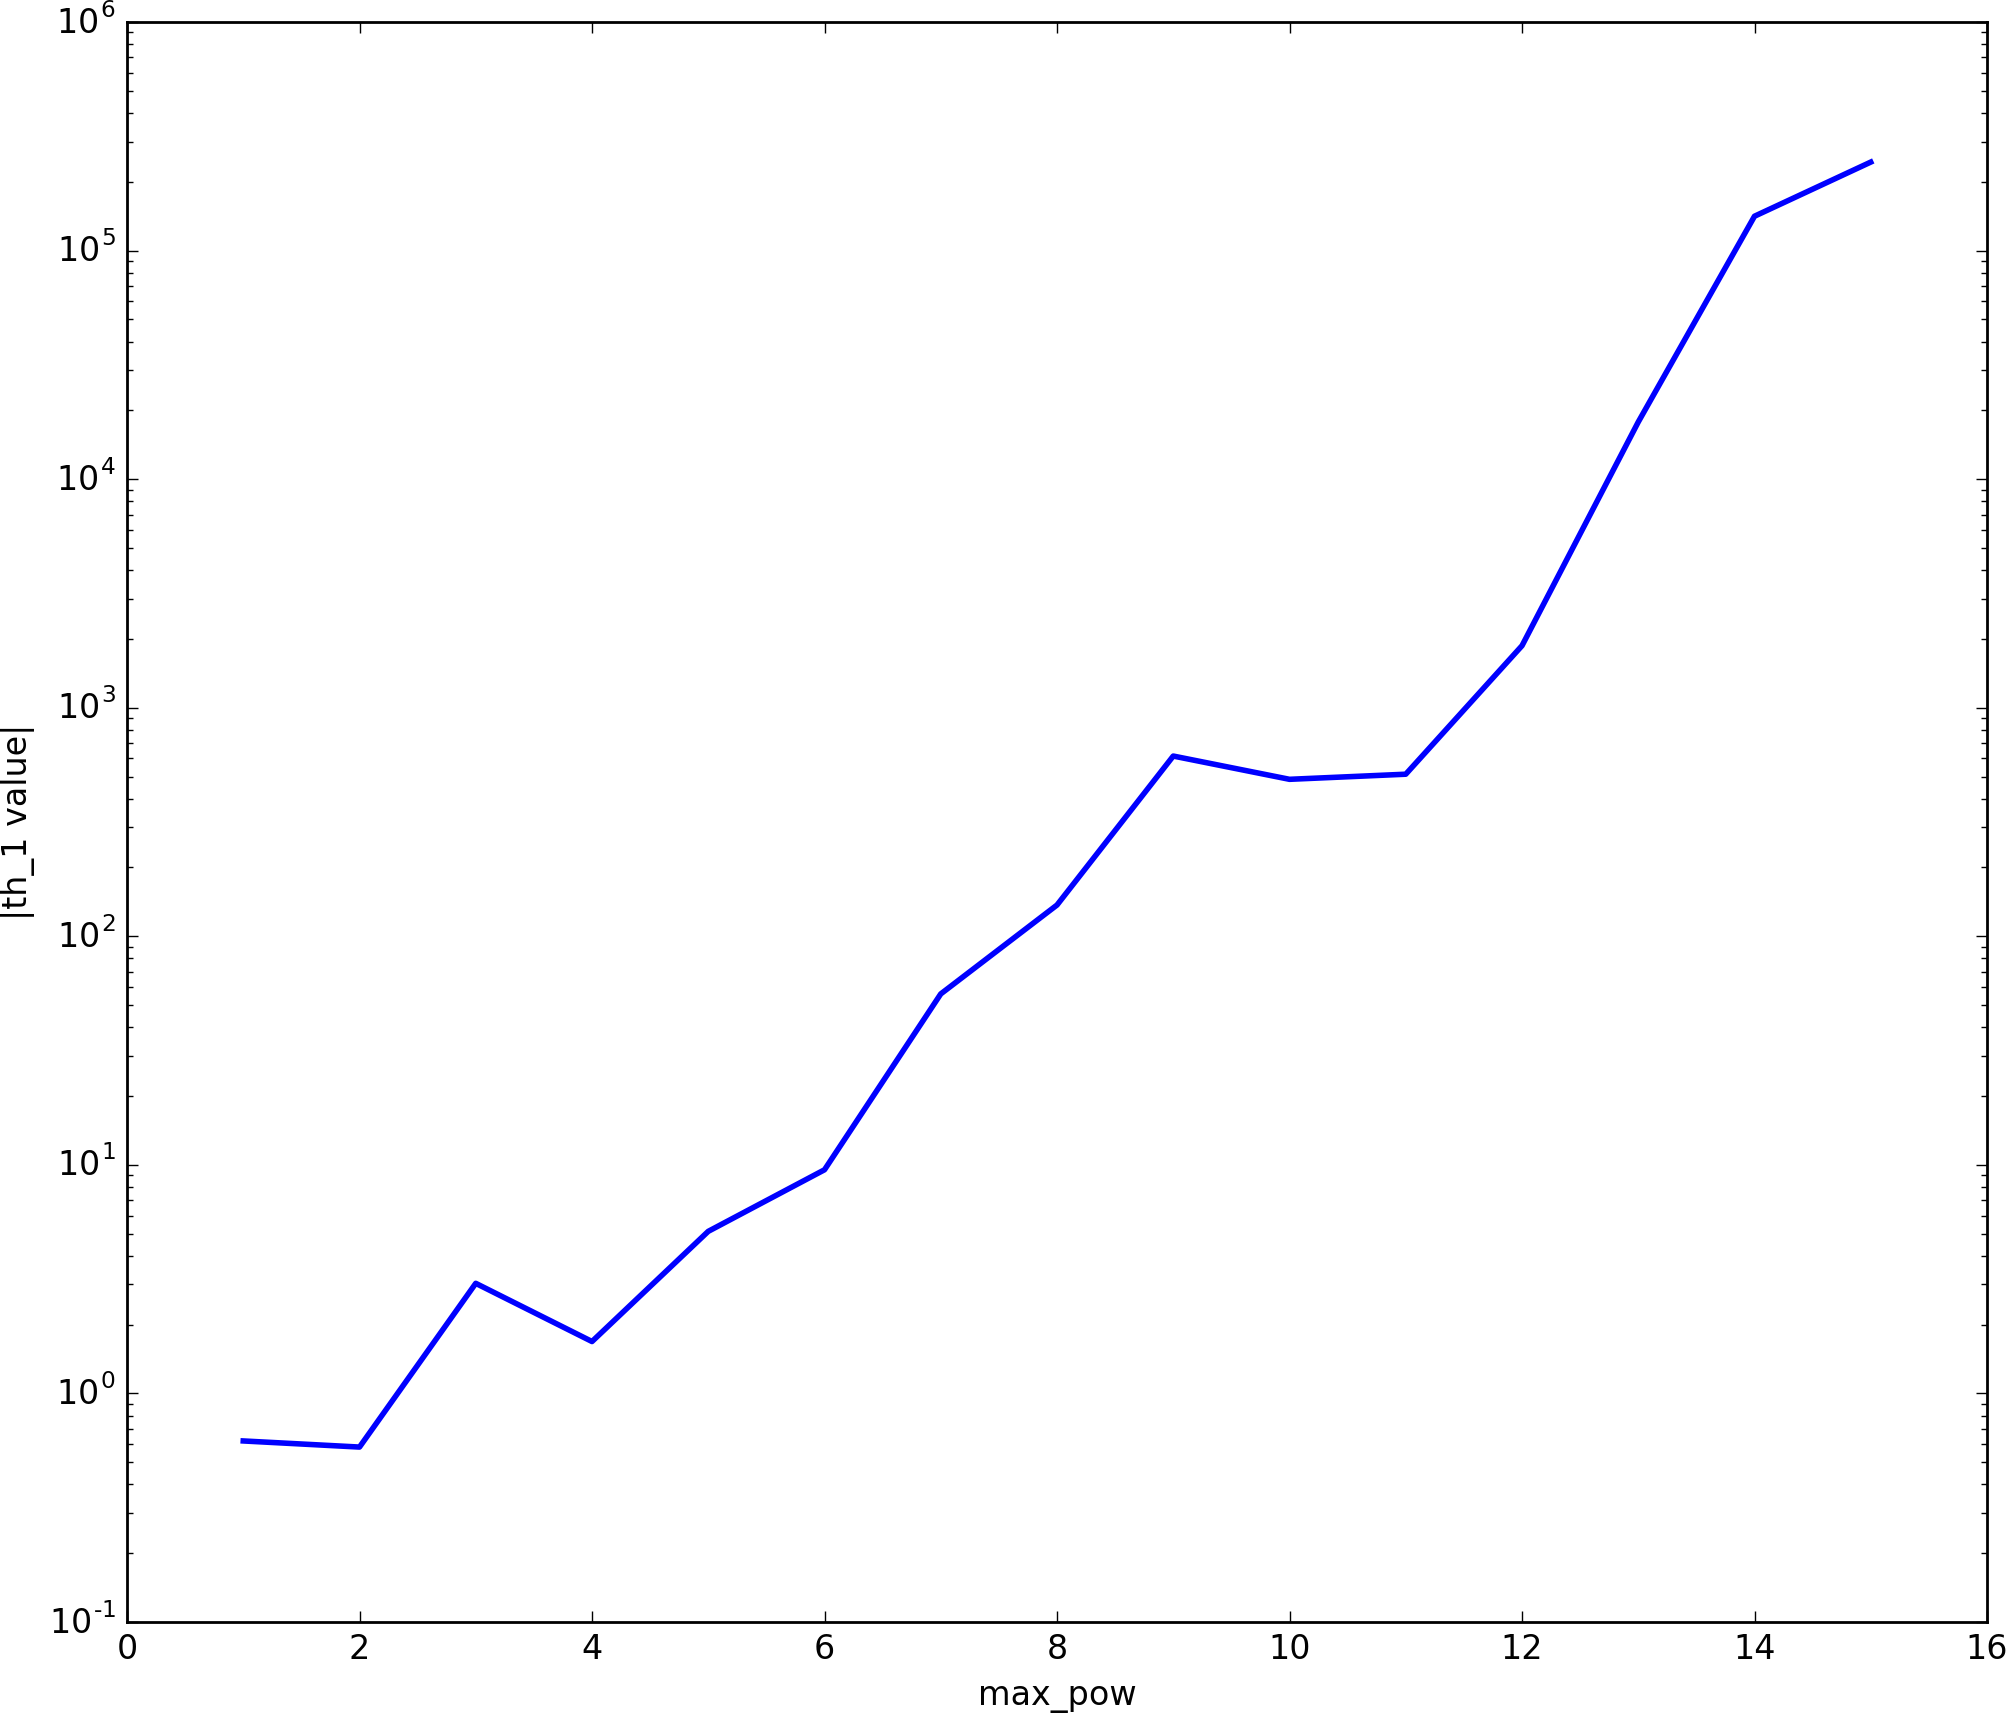
\includegraphics[height=0.75\textheight]{./fig/L1/coefs_th1.png}
\end{figure}

\end{frame}

%%%%%%%%%%%%%%%%%%%%%
\begin{frame}
\frametitle{Regularization}
\begin{block}{The idea}
The idea of regularization is to perform a regression minimizing a cost function
that includes a term to penalize "big" values for the parameters:
$$
J(\bm{\theta}) = \frac{1}{n} \sum (y_i - h_{\bm{\theta}}(x_i))^2 + \alpha P(\bm{\theta})
$$
\end{block}
\pause
We consider two penalty terms:
\begin{itemize}[<+->]
\item \alert{Ridge Regularization:} $P(\bm{\theta}) = \sum_{i=0}^p \theta_i^2$
\item \alert{Lasso Regularization:} $P(\bm{\theta}) = \sum_{i=0}^p |\theta_i|$
\item Elastic Net combines both regularization
\end{itemize}

\end{frame}

%%%%%%%%%%%%%%%%%%%%
\begin{frame}
\frametitle{Ridge regression}
\begin{block}{}
Ridge regression is a linear regression with a Ridge regularization:
$$
J(\bm{\theta}) = \frac{1}{n} \sum (y_i - h_{\bm{\theta}}(x_i))^2 + \alpha \sum_{i=0}^p \theta_i^2
$$
\end{block}
\end{frame}

%%%%%%%%%%%%%%%%%%%%
\begin{frame}
\frametitle{Results for $p=15$ and varying $\alpha$}
\begin{columns}
\column{.33\textwidth}
\vspace{-2em}
\begin{figure}
$\alpha=0$
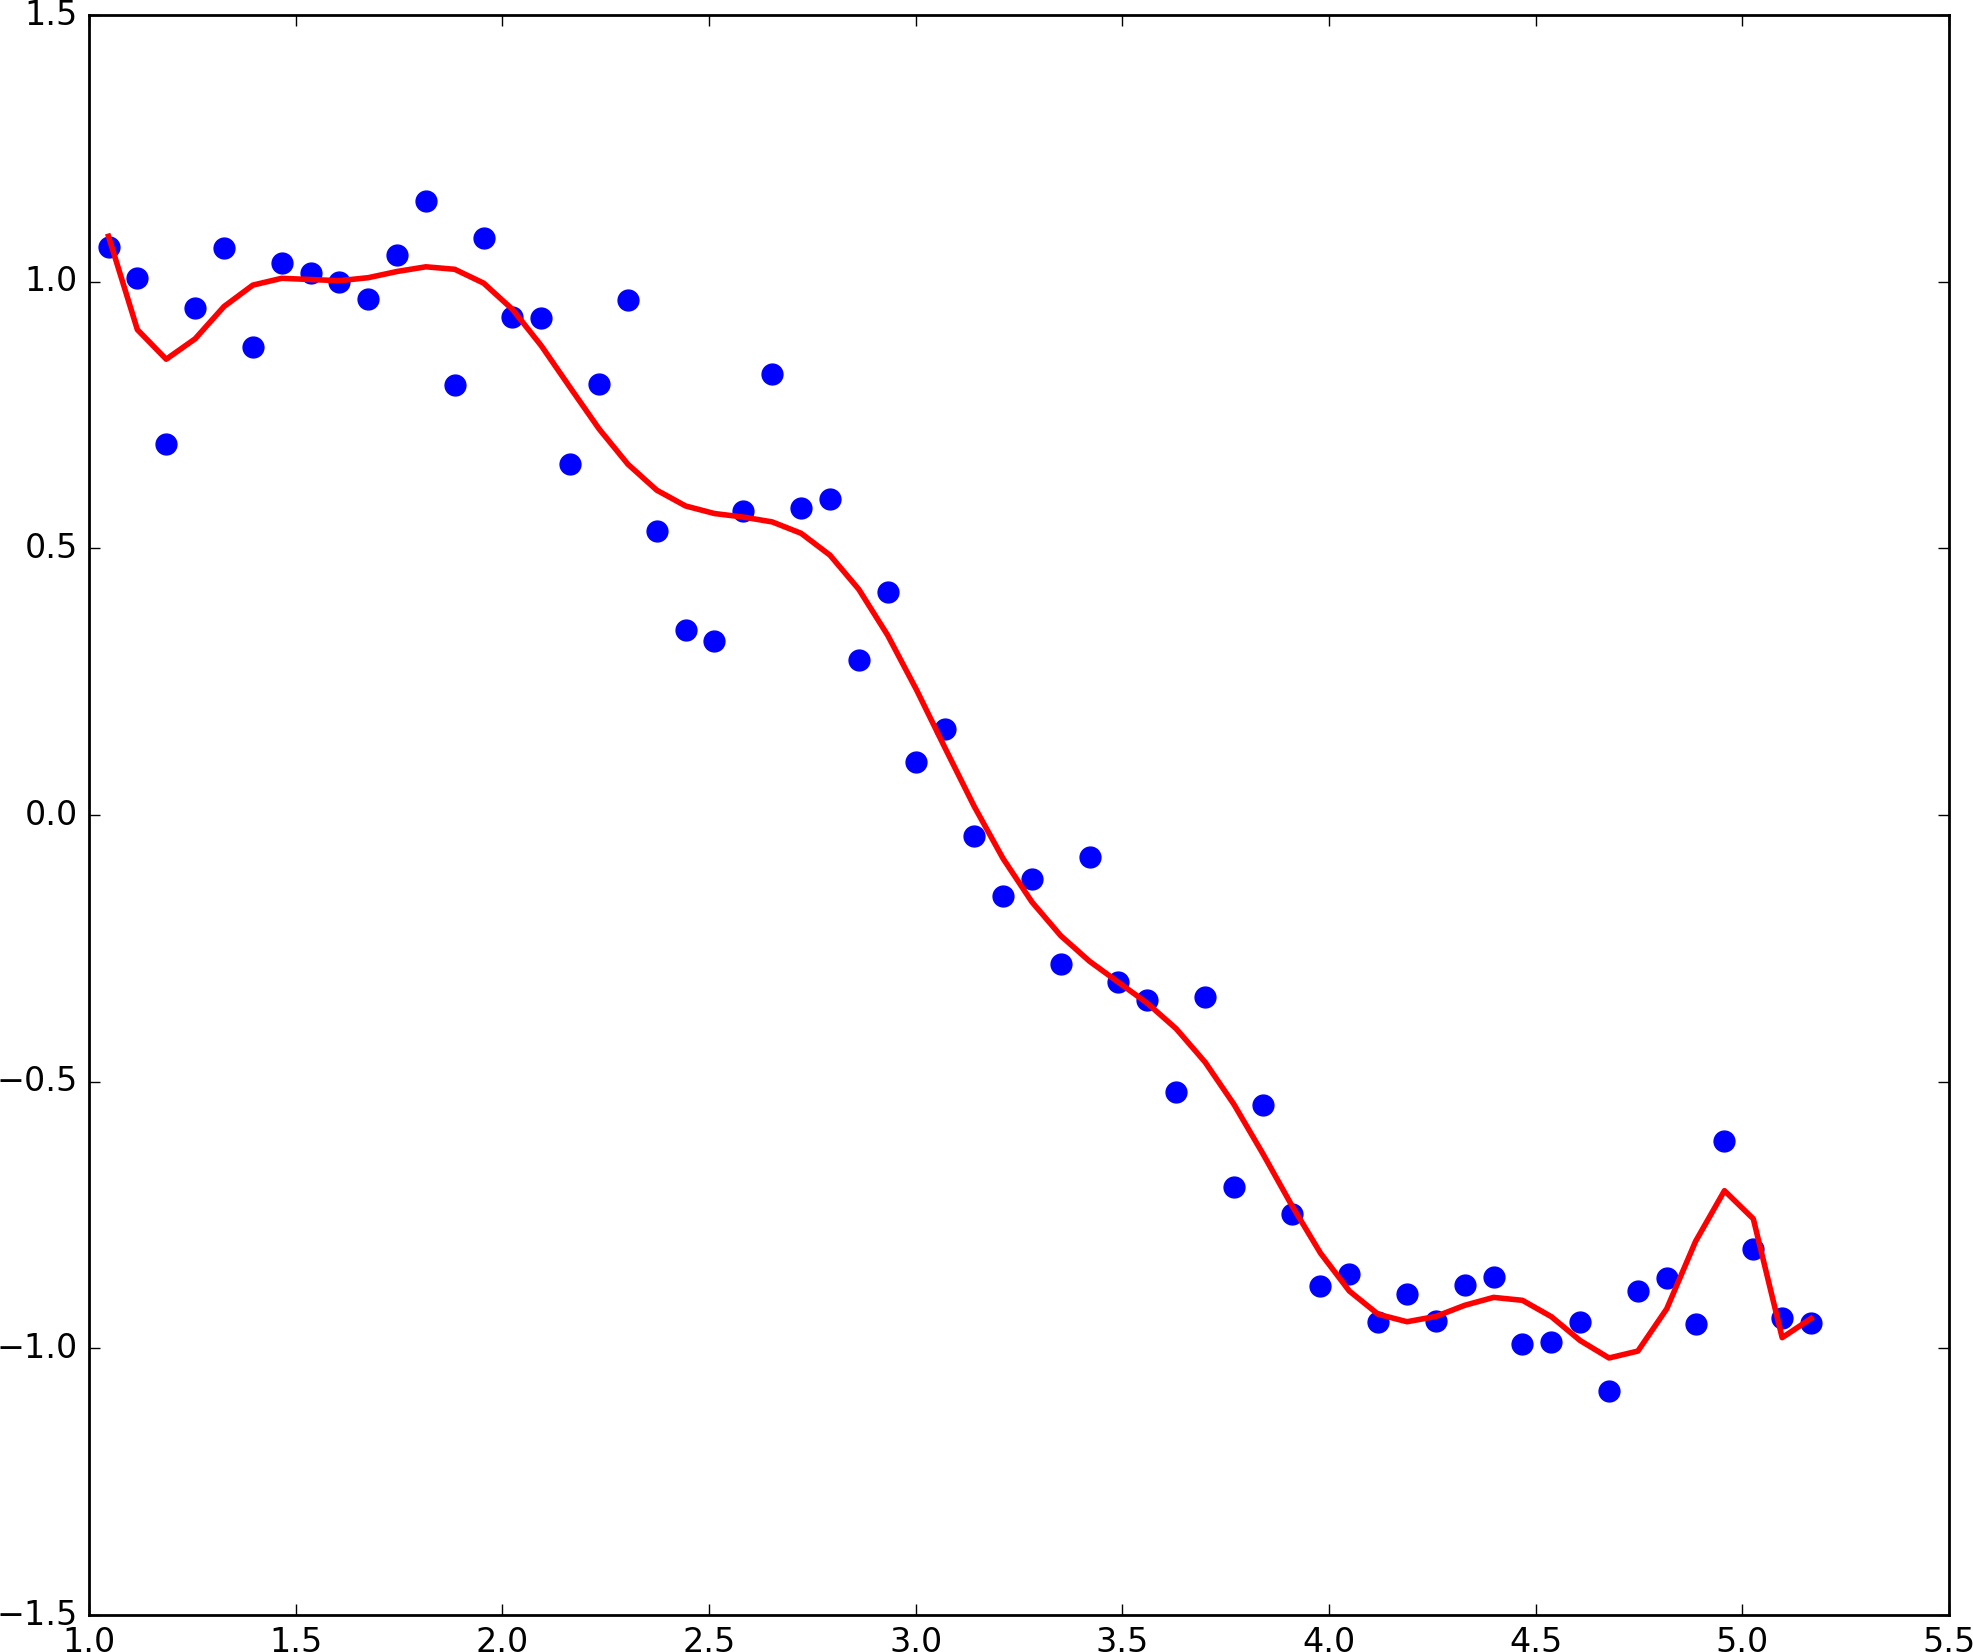
\includegraphics[width=0.99\textwidth]{./fig/L1/ridge_alpha0.png}
\end{figure}
\vspace{-2em}
\begin{figure}
$\alpha=1e-3$
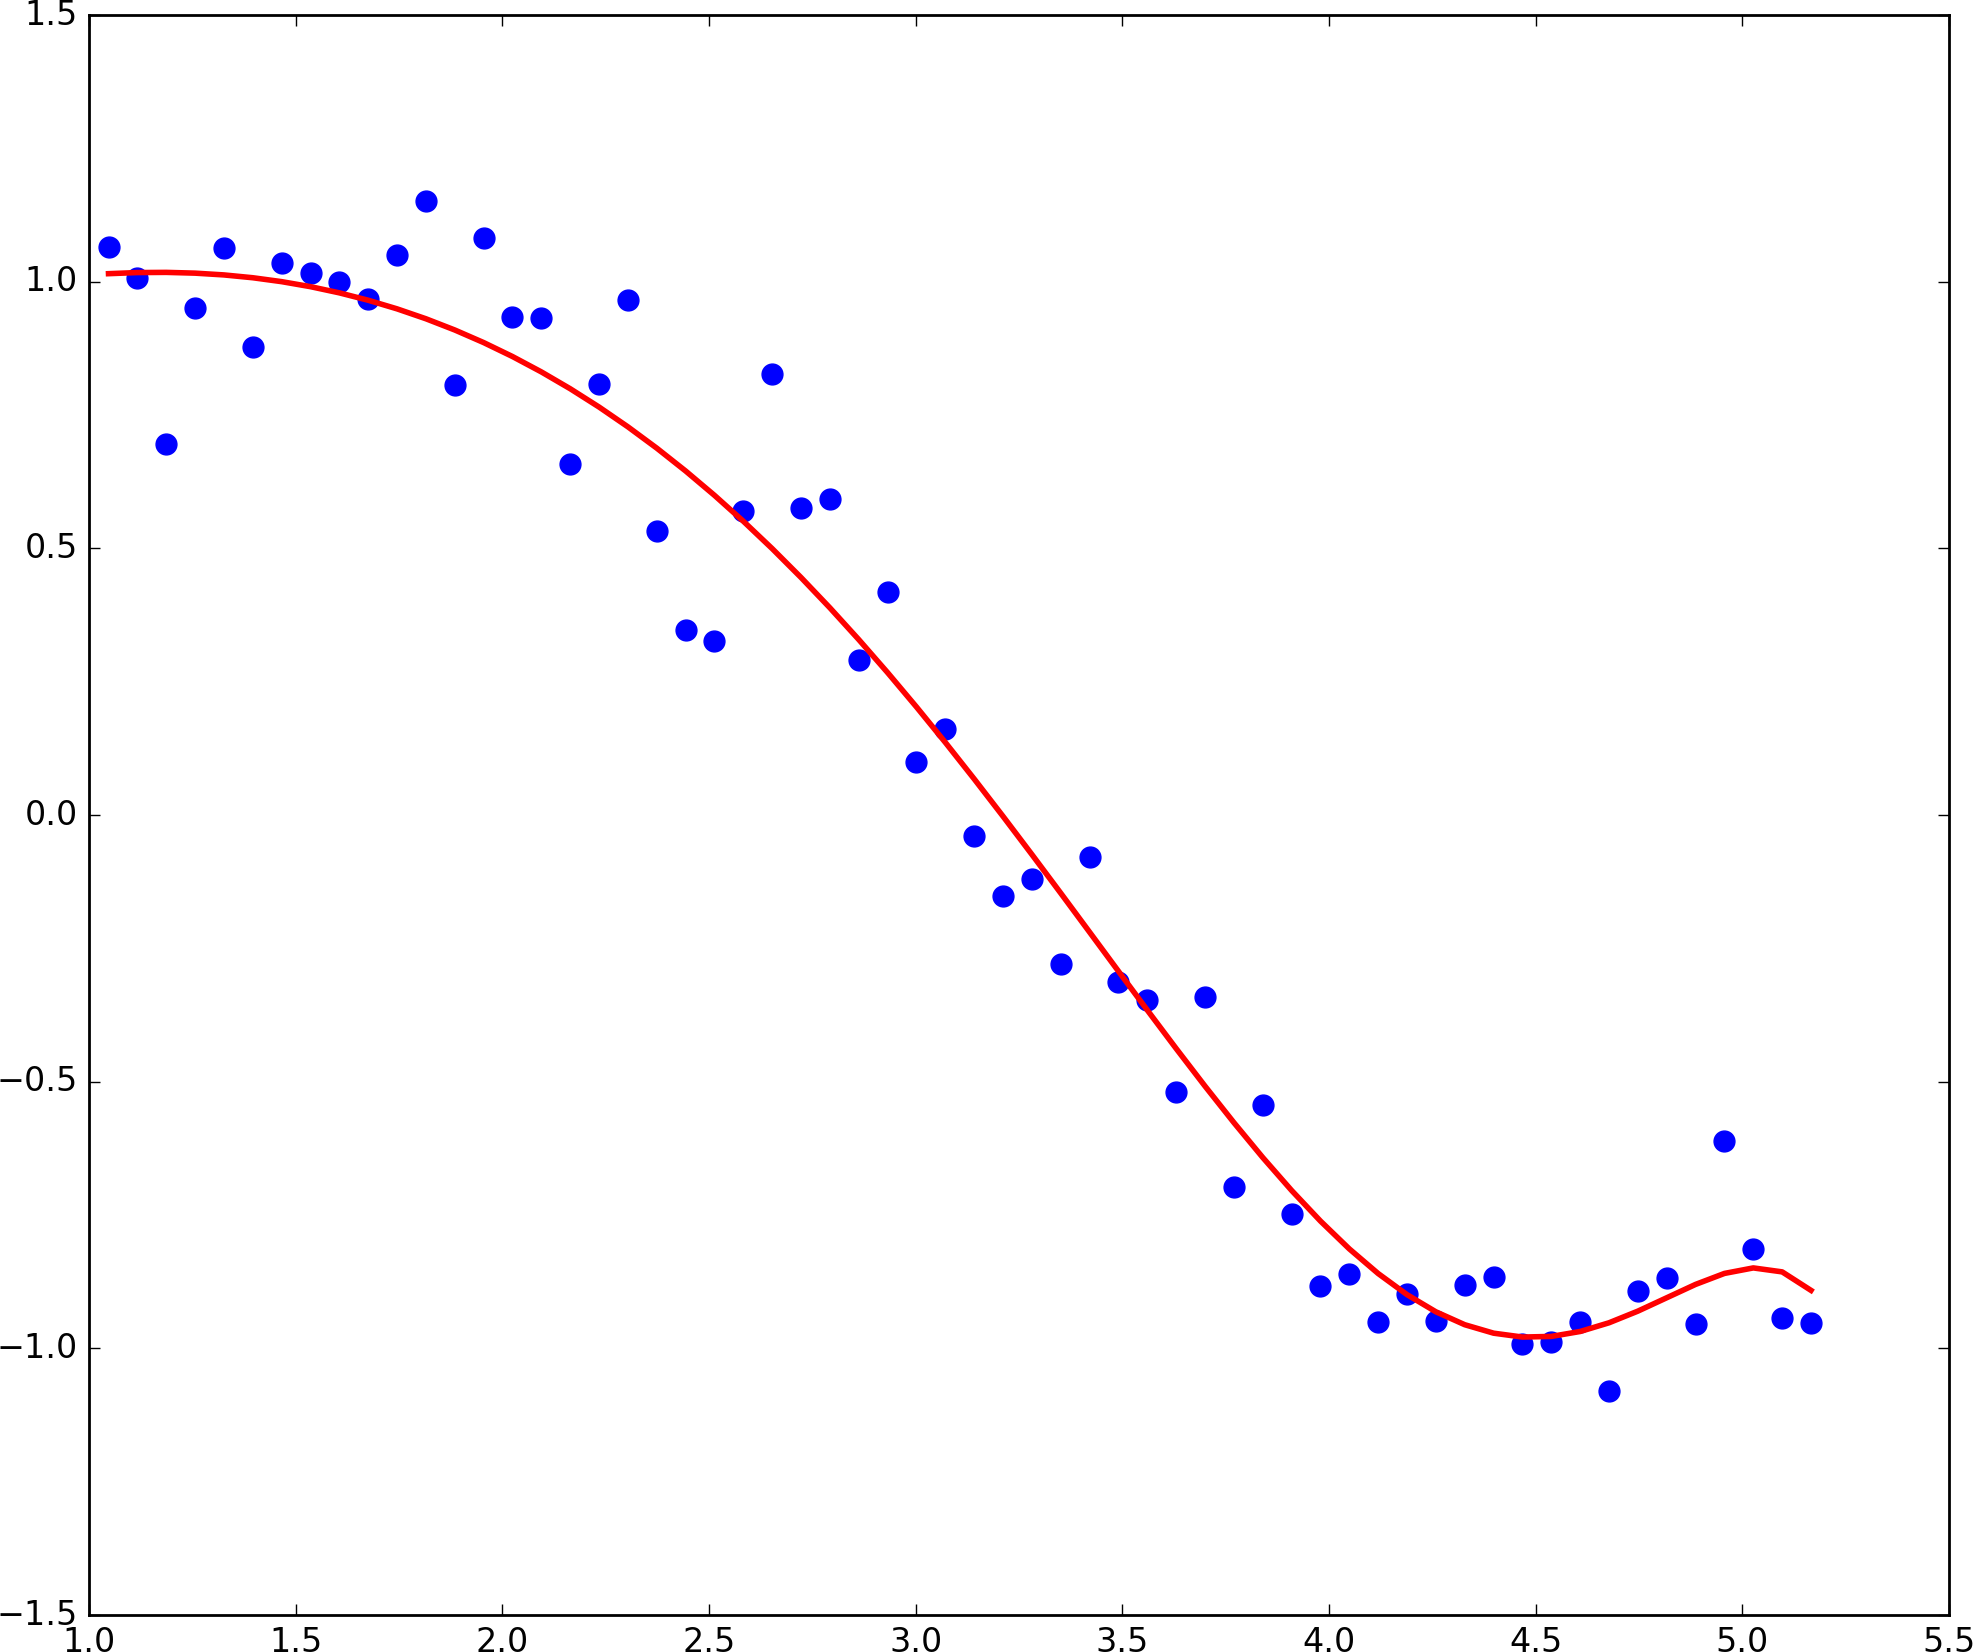
\includegraphics[width=0.99\textwidth]{./fig/L1/ridge_alpha1e-3.png}
\end{figure}
\column{.33\textwidth}
\vspace{-2em}
\begin{figure}
$\alpha=1e-15$
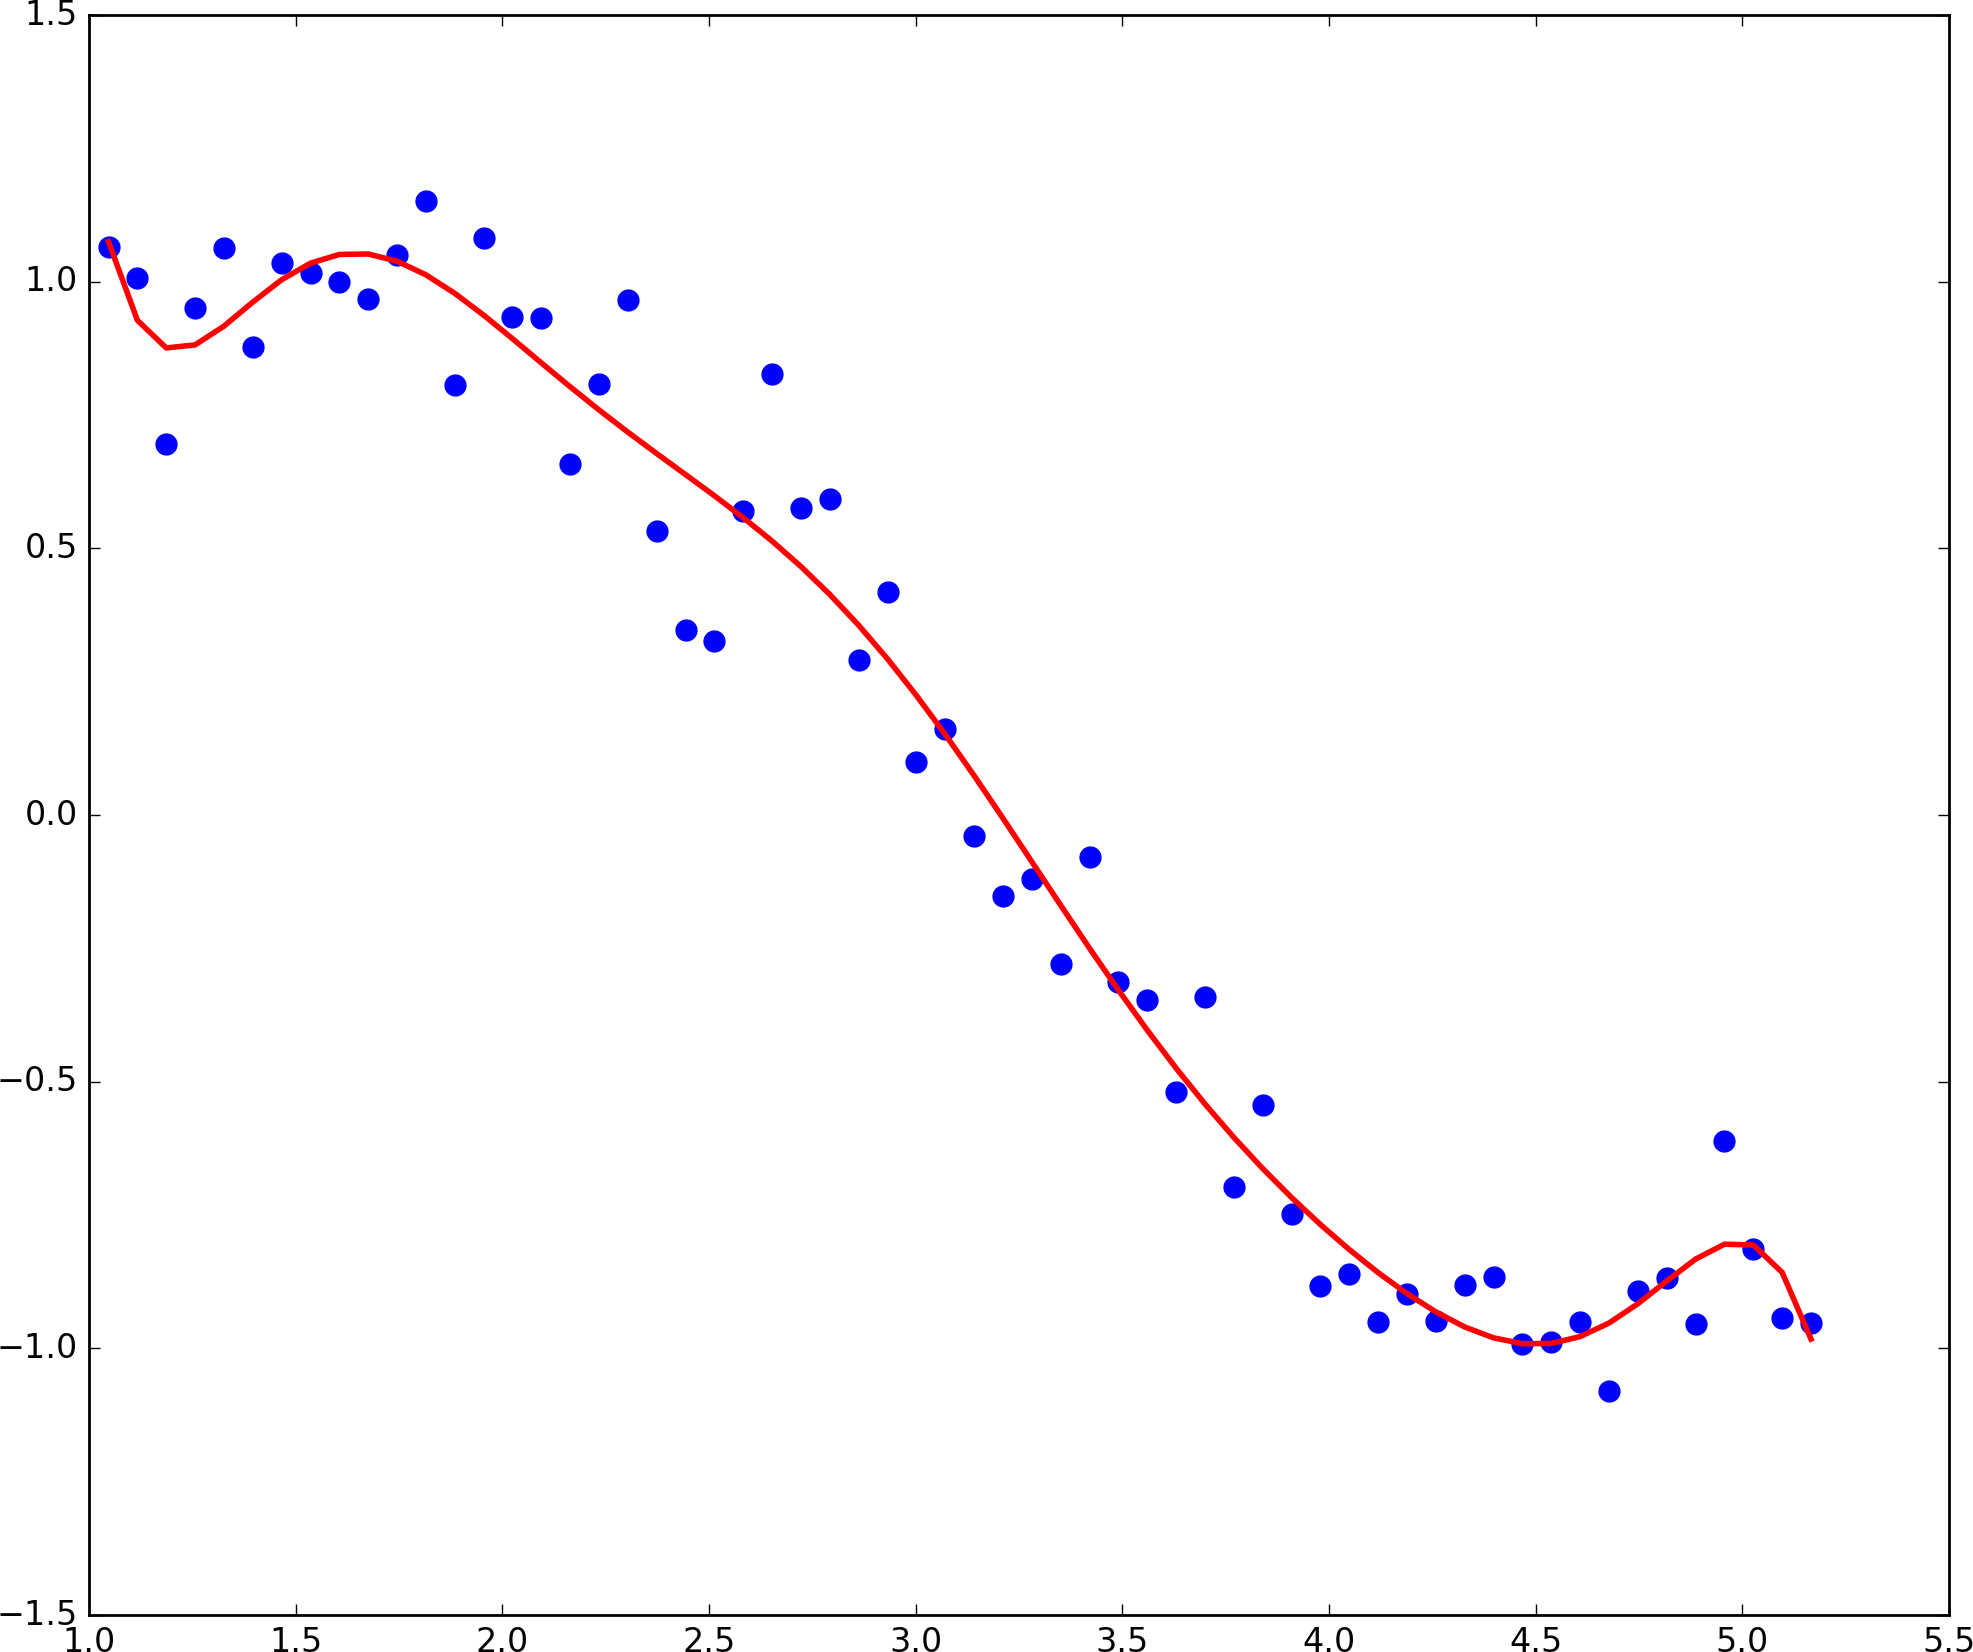
\includegraphics[width=0.99\textwidth]{./fig/L1/ridge_alpha1e-15.png}
\end{figure}
\vspace{-2em}
\begin{figure}
$\alpha=1e-2$
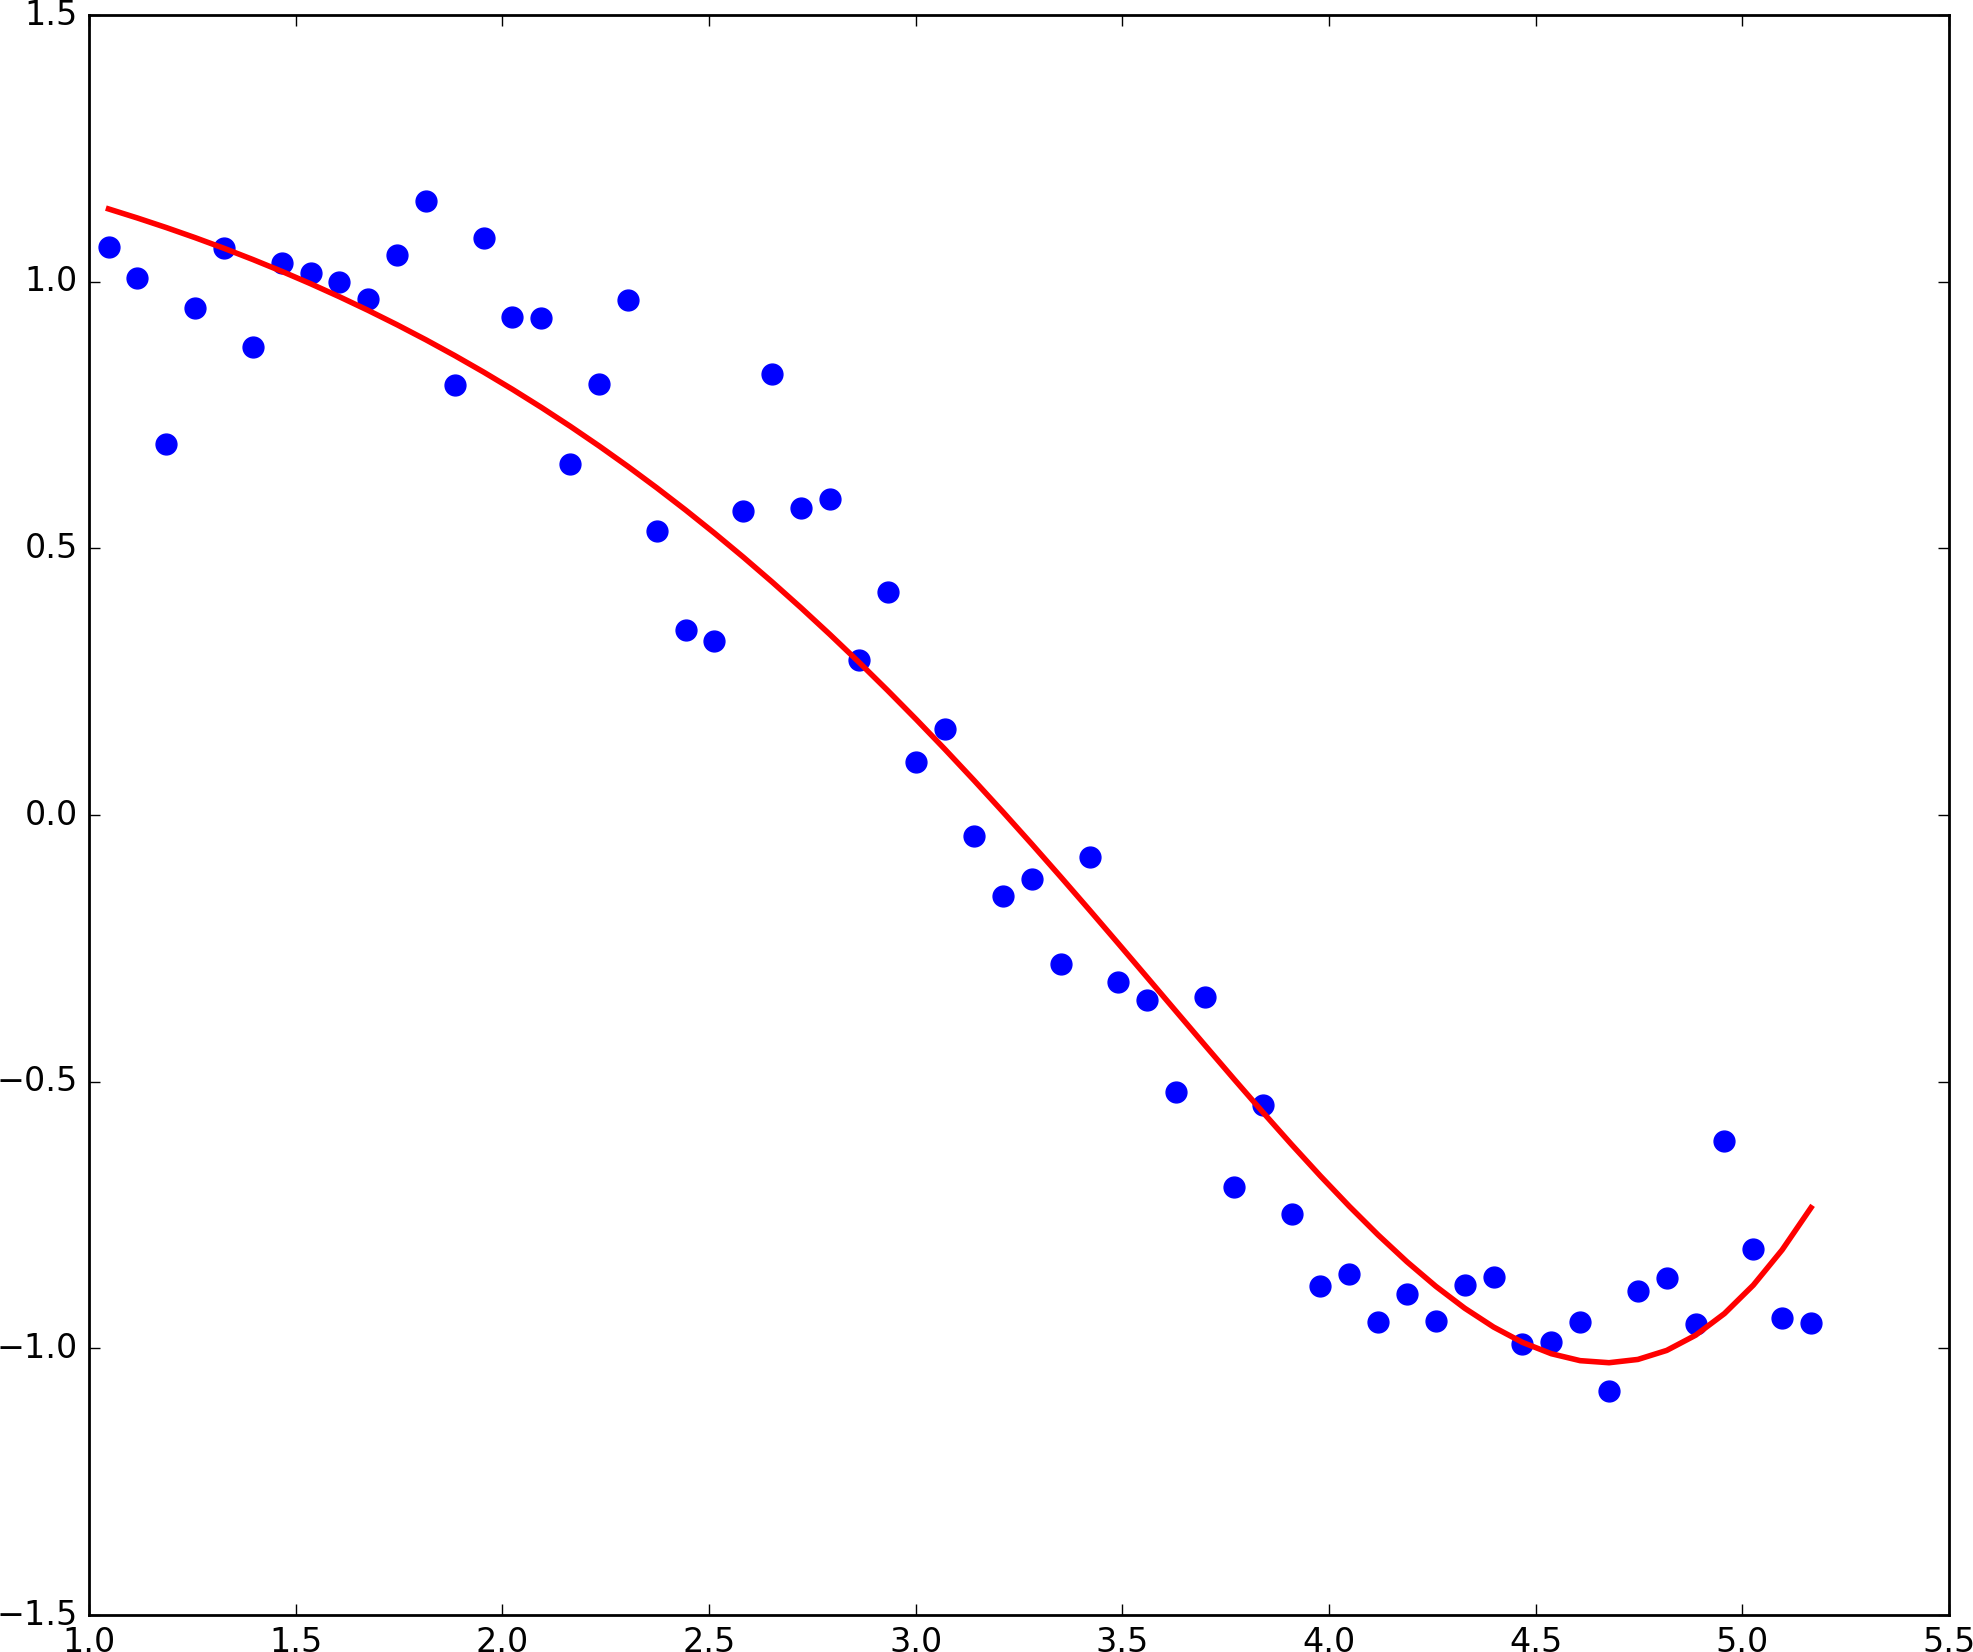
\includegraphics[width=0.99\textwidth]{./fig/L1/ridge_alpha1e-2.png}
\end{figure}
\column{.33\textwidth}
\vspace{-2em}
\begin{figure}
$\alpha=1e-4$
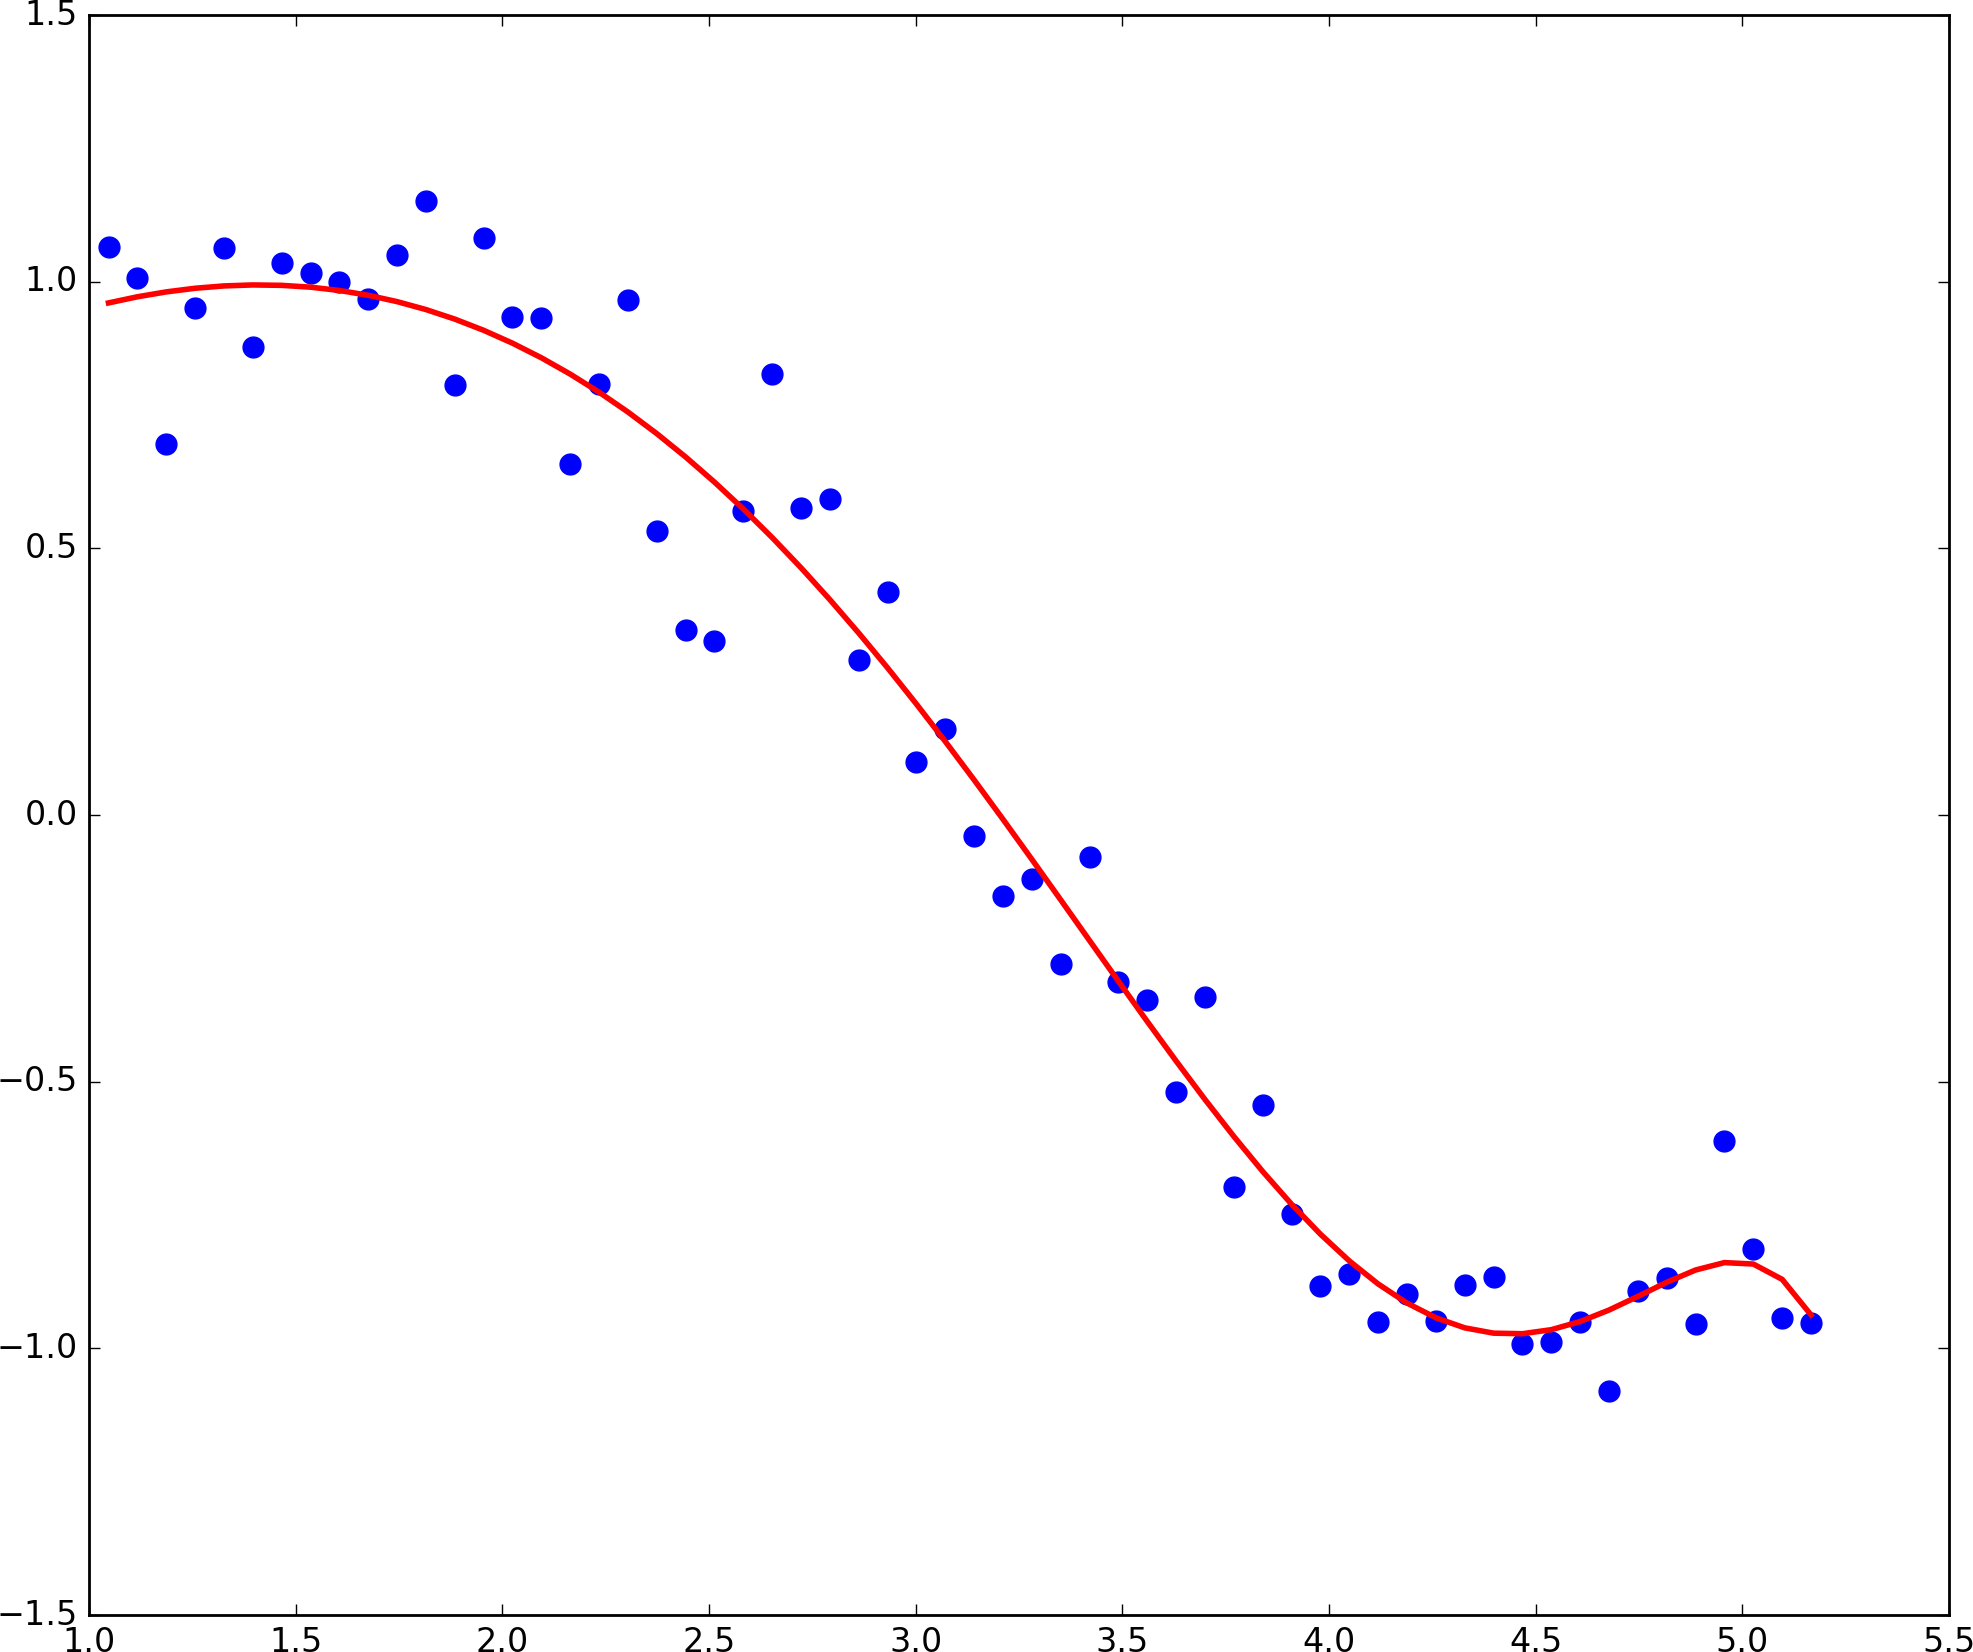
\includegraphics[width=0.99\textwidth]{./fig/L1/ridge_alpha1e-4.png}
\end{figure}
\vspace{-2em}
\begin{figure}
$\alpha=5$
\includegraphics[width=0.99\textwidth]{./fig/L1/ridge_alpha5.png}
\end{figure}
\end{columns}
\end{frame}

%%%%%%%%%%%%%%%%%%%%%
\begin{frame}
\frametitle{Values of coefficients}
\vspace{-2em}
\begin{table}
\resizebox{\textwidth}{!}{%
\begin{tabular}{lllllllllll}
\toprule
{} &      rmse &      th\_0 &      th\_1 &      th\_2 &      th\_3 &      th\_4 &      th\_5 &      th\_6 &      th\_7 &      th\_8 \\
\midrule
alpha\_0      & +1.17e-02 & -3.62e+04 & +2.44e+05 & -7.46e+05 & +1.38e+06 & -1.71e+06 & +1.53e+06 & -1.00e+06 & +4.98e+05 & -1.88e+05 \\
alpha\_1e-15  & +1.46e-02 & +9.43e+01 & -2.98e+02 & +3.79e+02 & -2.37e+02 & +6.72e+01 & -2.60e-01 & -4.35e+00 & +5.62e-01 & +1.42e-01 \\
alpha\_1e-10  & +1.54e-02 & +1.12e+01 & -2.90e+01 & +3.11e+01 & -1.52e+01 & +2.89e+00 & +1.69e-01 & -9.10e-02 & -1.08e-02 & +1.98e-03 \\
alpha\_1e-08  & +1.58e-02 & +1.34e+00 & -1.53e+00 & +1.75e+00 & -6.80e-01 & +3.88e-02 & +1.58e-02 & +1.59e-04 & -3.60e-04 & -5.37e-05 \\
alpha\_0.0001 & +1.60e-02 & +5.61e-01 & +5.47e-01 & -1.28e-01 & -2.57e-02 & -2.82e-03 & -1.10e-04 & +4.06e-05 & +1.52e-05 & +3.65e-06 \\
alpha\_0.001  & +1.67e-02 & +8.18e-01 & +3.05e-01 & -8.67e-02 & -2.05e-02 & -2.84e-03 & -2.19e-04 & +1.81e-05 & +1.24e-05 & +3.43e-06 \\
alpha\_0.01   & +2.39e-02 & +1.30e+00 & -8.84e-02 & -5.15e-02 & -1.01e-02 & -1.41e-03 & -1.32e-04 & +7.23e-07 & +4.14e-06 & +1.30e-06 \\
alpha\_1      & +9.41e-02 & +9.69e-01 & -1.39e-01 & -1.93e-02 & -3.00e-03 & -4.66e-04 & -6.97e-05 & -9.90e-06 & -1.29e-06 & -1.43e-07 \\
alpha\_5      & +2.31e-01 & +5.48e-01 & -5.89e-02 & -8.52e-03 & -1.42e-03 & -2.41e-04 & -4.08e-05 & -6.87e-06 & -1.15e-06 & -1.91e-07 \\
alpha\_10     & +3.00e-01 & +4.00e-01 & -3.72e-02 & -5.53e-03 & -9.50e-04 & -1.67e-04 & -2.96e-05 & -5.23e-06 & -9.25e-07 & -1.63e-07 \\
alpha\_20     & +3.79e-01 & +2.77e-01 & -2.25e-02 & -3.40e-03 & -5.99e-04 & -1.08e-04 & -1.97e-05 & -3.60e-06 & -6.58e-07 & -1.20e-07 \\
\bottomrule
\end{tabular}
}
\end{table}
\begin{figure}
\includegraphics[height=0.4\textheight]{./fig/L1/coefs_th5_ridge.png}\\
Value of $\theta_5$
\end{figure}
\end{frame}

%%%%%%%%%%%%%%%%%
\begin{frame}
\frametitle{Determination of the parameters in the ridge regression}
Considering the cost function J:
$$
J(\bm{\theta}) =J_{lms}(\bm{\theta}) + \alpha \sum_{i=0}^p \theta_i^2
$$
In a gradient algorithm, update of the parameters:

$\theta^{k+1}_i = \theta^k_i - \nu.(\frac{\partial J_{lms}}{D\theta_i} - 2\alpha\theta^k_i)$

So the update rule is:
$$
\theta^{k+1}_i = \theta^k_i(1-2 \nu \alpha) - \Delta_{lms}
$$
where
$\Delta_{lms}$ is the update in case of non-regularized regression

\end{frame}


%%%%%%%%%%%%%%%%%%%%
\begin{frame}
\frametitle{Lasso regression}
\begin{block}{}
Lasso regression is a linear regression with a Lasso regularization:
$$
J(\bm{\theta}) = \frac{1}{n} \sum (y_i - h_{\bm{\theta}}(x_i))^2 + \alpha \sum_{i=0}^p |\theta_i
$$
\end{block}
\end{frame}

%%%%%%%%%%%%%%%%%%%%
\begin{frame}
\frametitle{Results for $p=15$ and varying $\alpha$}
\begin{columns}
\column{.33\textwidth}
\vspace{-2em}
\begin{figure}
$\alpha=0$
\includegraphics[width=0.99\textwidth]{./fig/L1/lasso_alpha0.png}
\end{figure}
\vspace{-2em}
\begin{figure}
$\alpha=1e-3$
\includegraphics[width=0.99\textwidth]{./fig/L1/lasso_alpha1e-3.png}
\end{figure}
\column{.33\textwidth}
\vspace{-2em}
\begin{figure}
$\alpha=1e-15$
\includegraphics[width=0.99\textwidth]{./fig/L1/lasso_alpha1e-15.png}
\end{figure}
\vspace{-2em}
\begin{figure}
$\alpha=1e-2$
\includegraphics[width=0.99\textwidth]{./fig/L1/lasso_alpha1e-2.png}
\end{figure}
\column{.33\textwidth}
\vspace{-2em}
\begin{figure}
$\alpha=1e-4$
\includegraphics[width=0.99\textwidth]{./fig/L1/lasso_alpha1e-4.png}
\end{figure}
\vspace{-2em}
\begin{figure}
$\alpha=5$
\includegraphics[width=0.99\textwidth]{./fig/L1/lasso_alpha5.png}
\end{figure}
\end{columns}
\end{frame}

%%%%%%%%%%%%%%%%%%%%%
\begin{frame}
\frametitle{Values of coefficients}
\vspace{-2em}
\begin{table}
\resizebox{\textwidth}{!}{%
\begin{tabular}{lllllllllll}
\toprule
{} &      rmse &      th\_0 &      th\_1 &      th\_2 &      th\_3 &      th\_4 &      th\_5 &      th\_6 &      th\_7 &      th\_8 \\
\midrule
alpha\_0      & +1.17e-02 & -3.62e+04 & +2.44e+05 & -7.46e+05 & +1.38e+06 & -1.71e+06 & +1.53e+06 & -1.00e+06 & +4.98e+05 & -1.88e+05 \\
alpha\_1e-15  & +1.59e-02 & +2.22e-01 & +1.06e+00 & -3.69e-01 & +8.85e-04 & +1.63e-03 & -1.19e-04 & -6.44e-05 & -6.28e-06 & +1.45e-06 \\
alpha\_1e-10  & +1.59e-02 & +2.22e-01 & +1.06e+00 & -3.69e-01 & +8.84e-04 & +1.63e-03 & -1.18e-04 & -6.44e-05 & -6.28e-06 & +1.45e-06 \\
alpha\_1e-08  & +1.59e-02 & +2.22e-01 & +1.06e+00 & -3.69e-01 & +7.69e-04 & +1.62e-03 & -1.10e-04 & -6.45e-05 & -6.32e-06 & +1.43e-06 \\
alpha\_0.0001 & +1.72e-02 & +9.03e-01 & +1.71e-01 & -0.00e+00 & -4.78e-02 & -0.00e+00 & -0.00e+00 & +0.00e+00 & +0.00e+00 & +9.47e-06 \\
alpha\_0.001  & +2.80e-02 & +1.29e+00 & -0.00e+00 & -1.26e-01 & -0.00e+00 & -0.00e+00 & -0.00e+00 & +0.00e+00 & +0.00e+00 & +0.00e+00 \\
alpha\_0.01   & +6.07e-02 & +1.76e+00 & -5.52e-01 & -5.62e-04 & -0.00e+00 & -0.00e+00 & -0.00e+00 & -0.00e+00 & -0.00e+00 & -0.00e+00 \\
alpha\_1      & +6.16e-01 & +3.80e-02 & -0.00e+00 & -0.00e+00 & -0.00e+00 & -0.00e+00 & -0.00e+00 & -0.00e+00 & -0.00e+00 & -0.00e+00 \\
alpha\_5      & +6.16e-01 & +3.80e-02 & -0.00e+00 & -0.00e+00 & -0.00e+00 & -0.00e+00 & -0.00e+00 & -0.00e+00 & -0.00e+00 & -0.00e+00 \\
alpha\_10     & +6.16e-01 & +3.80e-02 & -0.00e+00 & -0.00e+00 & -0.00e+00 & -0.00e+00 & -0.00e+00 & -0.00e+00 & -0.00e+00 & -0.00e+00 \\
alpha\_20     & +6.16e-01 & +3.80e-02 & -0.00e+00 & -0.00e+00 & -0.00e+00 & -0.00e+00 & -0.00e+00 & -0.00e+00 & -0.00e+00 & -0.00e+00 \\
\bottomrule
\end{tabular}
}
\end{table}
\begin{figure}
\includegraphics[height=0.4\textheight]{./fig/L1/coefs_th5_lasso.png}\\
Value of $\theta_5$
\end{figure}
\end{frame}

%%%%%%%%%%%%%%%%%%%%
\begin{frame}
\frametitle{Determination of the parameters in the lasso regression}
Considering the cost function J:
$$
J(\bm{\theta}) =J_{lms}(\bm{\theta}) + \alpha \sum_{i=0}^p |\theta_i|
$$
In a gradient algorithm, update of the parameters would be:

J is not differentiable.
If we consider $\theta_{lms} = \theta_i^k -\nu.\frac{\partial J_{lms}}{D\theta_i} $

The update rule is:
\begin{itemize}
\item $\theta_i^{k+1} = \theta_{lms} + \alpha \nu$  if $\theta_{lms} < -\alpha \nu$
\item $\theta_i^k = 0$ if $-\alpha \nu < \theta_{lms} < \alpha \nu$
\item $\theta_i^{k+1} = \theta_{lms} - \alpha \nu$  if $\theta_{lms} > \alpha \nu$
\end{itemize}
\end{frame}

%%%%%%%%%%%%%%%%%%%%
\begin{frame}
\frametitle{Summary of parameters updates}
\begin{figure}
\includegraphics[height=0.8\textheight]{./fig/L1/updates.png}
\end{figure}
\end{frame}

%%%%%%%%%%%%%%%%%%%%%
\begin{frame}
\frametitle{Comparison Ridge/Lasso}
\begin{exampleblock}{ridge}
\begin{itemize}
\item Prevents the overfitting
\item includes all the features (dimensions) of the predictor, 
so it can be useless for high dimensional predictors
\end{itemize}
\end{exampleblock}
\pause
\begin{alertblock}{lasso}
\begin{itemize}
\item Provides sparse solutions and reduce the dimension of the
predictor
\item If some features in the predictor are correlated, arbitrarily select
one from the others.
\end{itemize}
\end{alertblock}
\end{frame}
%%%%%%%%%%%%%%%%%%%%%
\begin{frame}
\frametitle{Model Selection}
\begin{alertblock}{The "big" question}
How to determine some "hyper-parameter" of our model ?

examples: $\alpha$ for regularization, degree of polynomials
\end{alertblock}
\pause
The common approach:
\begin{enumerate}[<+->]
\item Split the dataset in two dataset : training and test
\item Optimize the parameters on the training dataset for a range of models (e.g. several values of $\alpha$)
\item Select the model with a lowest error on the test dataset
\end{enumerate}
\end{frame}
 
%%%%%%%%%%%%%%%%%%%%%
\begin{frame}
\frametitle{Test dataset}
\begin{columns}
\column{.5\textwidth}
\begin{figure}
The dataset:\\
\includegraphics[width=\textwidth]{./fig/L1/scatter_test.png}
\end{figure}
\pause
\column{.5\textwidth}
\begin{figure}
Error on the training and the test
with respect with $\alpha$
\includegraphics[width=\textwidth]{./fig/L1/validation.png}
\end{figure}

\end{columns}
\end{frame}



\begin{frame}
  \frametitle{Introduction to the percpetron}
  \begin{block}{}
  Introduced by Frank Rosenblatt ( July 11, 1928 - July 11, 1971) in 1957
  \end{block}
  \pause
  \begin{figure}
  \begin{tikzpicture}[
    basic/.style={draw,fill=blue!20,text width=1em,text badly centered},
    input/.style={basic,circle},
    weights/.style={basic,rectangle},
functions/.style={basic,circle,fill=blue!10},
]
        \node[functions] (center) {};
        \node[below of=center,font=\scriptsize,text width=4em] {Activation function};
        \draw[thick] (0.5em,0.5em) -- (0,0.5em) -- (0,-0.5em) -- (-0.5em,-0.5em);
      %  \draw (0em,0.75em) -- (0em,-0.75em);
      %  \draw (0.75em,0em) -- (-0.75em,0em);
        \node[right of=center, anchor = west] (right) {$y=$ 0 ou 1};
            \path[draw,->] (center) -- (right);
        \node[functions,left=3em of center] (left) {$\sum$};
            \path[draw,->] (left) -- (center);
%        \node[weights,left=3em of left] (2) {$w_2$} -- (2) 
            \node[input,left= 4em of left] (l2) {$x_2$};
%            \path[draw,->] (l2) -- (2);
            \path[draw,->] (l2) -- node[above,midway]{$w_2$}(left);
        \node[below of=l2] (dots) {$\vdots$} ;
%(dots) node[left of=dots] (ldots) {$\vdots$};
%        \node[weights,below of=dots] (n) {$w_n$} -- (n) 
\node[input,below of=dots] (ln) {$x_n$};
%            \path[draw,->] (ln) -- (n);
            \path[draw,->] (ln) -- node[above,midway]{$w_n$}(left);
%        \node[weights,above of=2] (1) {$w_1$} -- (1) 
            \node[input,above of=l2] (l1) {$x_1$};
%            \path[draw,->] (l1) -- (1);
            \path[draw,->] (l1) -- node[above,midway]{$w_1$}(left);
%        \node[weights,above of=1] (0) {$w_0$} -- (0) 
\node[input,above of=l1] (l0) {$1$};
%            \path[draw,->] (l0) -- (0);
            \path[draw,->] (l0) -- node[above,midway]{$w_0$}(left);
        \node[below of=ln,font=\scriptsize](lin) {inputs};
        \node[right of=lin,font=\scriptsize] {weights};
    \end{tikzpicture}
    \end{figure}
\begin{block}{}
If $w_0 + w_1 x_1 + w_2 x_2 +  \dots + w_n\ x_n < 0$, then $y=0$\\
else $y=1$
\end{block}
\end{frame}
\begin{frame}
\frametitle{Two different predictions}

\begin{columns}
\column{0.45\textwidth}
$w_0=$ \red{1}, $w_1=$ \red{-2},$w_2=$ \red{2}\\
\vspace{1em}

 \begin{tikzpicture}[
    basic/.style={draw,fill=blue!20,text width=1em,text badly centered},
    input/.style={basic,circle, text width=1em, inner sep=0},
    weights/.style={basic,rectangle},
functions/.style={basic,circle,fill=blue!10},
]
        \node[functions] (center) {};
        \draw[thick] (0.5em,0.5em) -- (0,0.5em) -- (0,-0.5em) -- (-0.5em,-0.5em);
        \node[right = 1em of center, anchor = west] (right) {$y=$ \red{1}};
            \path[draw,->] (center) -- (right);
        \node[functions,left=1em of center] (left) {$\sum$};
            \path[draw,->] (left) -- (center);
            \node[left= 2em of left] (l2) {$x_1=0$};
            \path[draw,->] (l2) -- node[above,midway]{$w_1$}(left);
            \node[below of=l2] (ln) {$x_2=1$};
            \path[draw,->] (ln) -- node[above,midway]{$w_2$}(left);
            \node[above of=l2] (l1) {$1$};
            \path[draw,->] (l1) -- node[above,midway]{$w_0$}(left);
           % \node[input,above of=l1] (l0) {$1$};
           % \path[draw,->] (l0) -- node[above,midway]{$w_0$}(left);
%        \node[below of=ln,font=\scriptsize](lin) {inputs};
%        \node[right of=lin,font=\scriptsize] {weights};
    \end{tikzpicture}

$$
w_0 + w_1 x_1 + w_2 x_2 = 3 > 0
$$

\column{0.45\textwidth}
$w_0=$ \red{1}, $w_1=$ \red{2},$w_2=$ \red{-2}\\
\vspace{1em}

 \begin{tikzpicture}[
    basic/.style={draw,fill=blue!20,text width=1em,text badly centered},
    input/.style={basic,circle, text width=1em, inner sep=0},
    weights/.style={basic,rectangle},
functions/.style={basic,circle,fill=blue!10},
]
        \node[functions] (center) {};
        \draw[thick] (0.5em,0.5em) -- (0,0.5em) -- (0,-0.5em) -- (-0.5em,-0.5em);
        \node[right = 1em of center, anchor = west] (right) {$y=$ \red{0}};
            \path[draw,->] (center) -- (right);
        \node[functions,left=1em of center] (left) {$\sum$};
            \path[draw,->] (left) -- (center);
            \node[left= 2em of left] (l2) {$x_1=0$};
            \path[draw,->] (l2) -- node[above,midway]{$w_1$}(left);
            \node[below of=l2] (ln) {$x_2=1$};
            \path[draw,->] (ln) -- node[above,midway]{$w_2$}(left);
            \node[above of=l2] (l1) {$1$};
            \path[draw,->] (l1) -- node[above,midway]{$w_0$}(left);
           % \node[input,above of=l1] (l0) {$1$};
           % \path[draw,->] (l0) -- node[above,midway]{$w_0$}(left);
%        \node[below of=ln,font=\scriptsize](lin) {inputs};
%        \node[right of=lin,font=\scriptsize] {weights};
    \end{tikzpicture}

$$
w_0 + w_1 x_1 + w_2 x_2 = -1 < 0
$$

\end{columns}


\end{frame}

\begin{frame}
\frametitle{Learning of the weights}
\framesubtitle{Supervised learning}
Training set: $\{(x_1,y_1),\ldots,(x_n,y_n)\}$

\begin{block}{Learning algorithm}
\begin{enumerate}[<+->]
\item Initialization of the weights $w_i$
\item We consider the data $(x_j,y_j)$
\item The perceptron predicts $\hat{y}_j$
\item Update of the weights:\\
$w_i=w_i- (\hat{y}_j - y_j)\times x_{ij}$
\item Back to step 2
\end{enumerate}
\end{block}

\end{frame}

\begin{frame}
\frametitle{Link between perceptron and Linear/logistic regression}

\begin{itemize}
\item weight in a perceptron $\Leftrightarrow$ parameters of a model
\item Activation function  $\Leftrightarrow$ hypothesis model
\item If the activation function is linear, perceptron performs a linear regression
\item If the activation function is a sigmoid, perceptron performs a logistic regression
\end{itemize}

\end{frame}

\end{document}